% REMEMBER: You must not plagiarise anything in your report. Be extremely careful.
\documentclass{l4proj}

    
%==============================================================================
% Put any additional packages here
% You can add any packages you want, as long as it does not alter
% the overall format (e.g. don't change the margins or the reference style).
%
\usepackage{pdfpages} % if you want to include a PDF for an ethics checklist, for example
\usepackage{longtable}
\usepackage{booktabs}
\usepackage{xcolor}
\usepackage{float}
\usepackage{adjustbox}
\usepackage{caption}
\usepackage{graphicx}
\usepackage{pifont}
\usepackage{titlesec}
\titlespacing*{\subsubsection}{0pt}{1em}{0.5em}
\usepackage{enumitem}



%
%

\begin{document}

%==============================================================================
%% METADATA
\title{Evergreen Budgeting: A Personal Budget Tracker} % change this to your title
\author{Kirsty Balfour}
\date{September 24, 2024}

\maketitle

%==============================================================================
%% ABSTRACT
\begin{abstract}
    Budgeting is an essential tool for maintaining financial stability, achieving personal savings goals, and building long-term financial resilience. While technology offers powerful means to support budgeting, existing tools are often either too flexible, resulting in complexity and users being overwhelmed, or too restrictive to accommodate user needs.

    This project focused on implementing a personal budgeting application called Evergreen Budgeting. It was built using Angular, Node.js, and a PostgreSQL database, and it allows users to create a category-based budget, log and track income and expenses, set and manage savings goals, and generate financial reports.
    
    The application was evaluated against its original requirements, focusing on usability, functionality, and overall experience. Results showed that most participants would prefer using Evergreen Budgeting over their current budgeting methods. However, issues related to mobile usability and the savings allocation approach were identified, highlighting key areas for future work.
\end{abstract}

%==============================================================================
%% ACKNOWLEDGEMENTS
\chapter*{Acknowledgements}

Firstly, I would like to thank my project supervisor, Dr Sofiat Olaosebikan, for the opportunity to take on this project and her constant help and support over these last six months. Secondly, thanks go to my academic advisor, Professor David Manlove, who was always willing to provide advice and feedback.

I would also like to thank all my friends and family for their encouragement and for always being there to talk things through when needed. Lastly, special thanks go to my mother, who patiently dealt with far too many phone calls throughout this project, and my father, who shared his financial expertise and provided valuable feedback on the app’s features and design.

%==============================================================================

\def\consentname {Kirsty Balfour} % your full name
\def\consentdate {24 September 2024} % the date you agree
%
\educationalconsent


%==============================================================================
\tableofcontents

%==================================================================================================================================

%==================================================================================================================================
\chapter{Introduction}

% reset page numbering. Don't remove this!
\pagenumbering{arabic} 

\section{Motivation}
Budgeting is a fundamental financial practice that allows individuals and families to manage their money effectively, enabling them to achieve personal goals such as saving for a holiday, purchasing a home, or preparing for retirement. At the same time, it plays a crucial role in day-to-day financial stability, helping people cover regular expenses, avoid debt, and handle unexpected costs. By providing a structured approach to tracking income and expenses, budgeting offers a sense of financial control and security, reducing uncertainty and stress \citep{shukri_personal_2024}.

Despite its importance, financial literacy is often overlooked in formal education, leaving many young people unprepared to manage their finances when they first become financially independent \citep{stillwell_financial_2016}. Without a foundational understanding of budgeting principles, individuals may struggle to develop effective money management habits, leading to financial stress and potential long-term difficulties.

Technology presents a powerful solution to this challenge by offering intuitive tools that simplify budgeting, automate expense tracking, and provide insightful spending analysis. Unlike traditional manual methods, such as paper-based tracking or wholly mental estimation, digital solutions can leverage automation and data-driven insights to improve financial awareness and decision-making \citep{sonjaya_exploring_2024}.

While various technological solutions already exist, such as spreadsheets and specialised budgeting applications, they come with notable drawbacks. Spreadsheets offer high customisability but can be overwhelming for users unfamiliar with either financial concepts or spreadsheet functionalities. Many budgeting apps, while simplifying the process, often lock essential features behind paywalls, focus primarily on reporting rather than budgeting, and tend to lack flexibility.

These limitations highlight the need for a new tool that finds a balance between usability and flexibility, providing an accessible, structured, and adaptable budgeting solution without complexity or cost barriers.

\section{Goals}

The aim of this project is to develop a mobile-friendly budgeting web application that enables users to track their spending, income, and savings goals while providing insightful financial analysis. The application should prioritise usability, flexibility, and accessibility, ensuring that both experienced budgeters and beginners can use it effectively.

To achieve this, the following key goals have been set:

\begin{itemize}
    \item Users should be able to log, edit, and delete income and expenses with relevant details, including categorisation for better financial tracking.
    \item The application should implement a category-based budgeting system, allowing users to allocate funds effectively and monitor their spending within set limits.
    \item Users should be able to set and track savings goals, helping them work towards both short-term and long-term financial objectives.
    \item The application should generate reports and visualisations, such as spending breakdowns and trend analyses, to help users understand their financial habits.
    \item The interface should be mobile-friendly, intuitive and easy to navigate, ensuring that both experienced budgeters and beginners can use the application effectively.
    \item The application should feature a secure login system to protect user data, ensuring that financial information remains private and accessible only to the user.
    \item User data should be stored persistently, allowing them to access their financial history even after logging out or switching devices.
    \item Users should be informed when they exceed their budget, overspend in specific categories, or need to plan for upcoming expenses.
\end{itemize}

By fulfilling these goals, the project aims to create a user-friendly, secure, and flexible budgeting tool that empowers individuals to take control of their day-to-day spending and long-term financial planning without complexity or cost barriers.


\section{Summary}
This dissertation presents the development of a budgeting application aimed at enhancing financial management. The remainder of this paper is structured as follows:

\begin{itemize}
    \item \textbf{Chapter 2} discusses the background and context of budgeting, exploring its importance in personal finance and examining how technology can address common challenges. It also provides a brief description of current solutions.
    \item \textbf{Chapter 3} details the analysis and requirements-gathering process, including idea generation, existing app analysis, user surveys, and MoSCoW prioritisation to establish the Minimal Viable Product (MVP) requirements.
    \item \textbf{Chapter 4} outlines the design of the system, covering the architecture, wireframes, database schema, and technology choices, while also discussing key design decisions.
    \item \textbf{Chapter 5} describes the implementation of the application, including software engineering practices, feature development, UI considerations, database integration, security measures, and deployment.
    \item \textbf{Chapter 6} evaluates the system’s features and reliability, presenting the results of a user study and aligning them with the initial project requirements. This chapter also discusses the testing approaches used.
    \item \textbf{Chapter 7} summarises the project outcomes, reflects on the development process, and suggests areas for future work to enhance the application’s capabilities.
\end{itemize}

\section{Relevant Links}
For the reader's convenience, relevant links can be found below:
\begin{itemize}
    \item Link to the hosted application: \url{https://evergreen-budgeting-app.web.app/}
    \item Link to the application repository: \url{https://github.com/kirstyb2003/evergreen-budgeting-app}
    \item Link to the project repository, containing meeting minutes, evaluation data, and other administrative documents: \url{https://github.com/kirstyb2003/Personal-Budget-Tracker}
\end{itemize}

%==================================================================================================================================
\chapter{Background}

\section{What is Budgeting and How is it Used?}
Budgeting, as defined by \citet{shim_budgeting_2011}, is the process of planning how to manage your finances in order to meet goals and needs. It involves setting spending limits, tracking income and expenses, and making deliberate decisions about how to use money over specific periods. While originally developed in the context of business budgets, applying Shim’s definitions to personal finances suggests that a budget can help people stay in control of their money, avoid overspending, prepare for future expenses, and ensure that their financial choices align with their priorities and goals.

There are several common methods for managing personal budgets. For example, the 50/20/30 rule, discussed by the University of Pennsylvania’s Financial Wellness section \citep{pen_popular_budget}, allocates 50\% of income to needs, 20\% to savings, and 30\% to wants. Another popular strategy is “Pay Yourself First,” where a predetermined amount is immediately set aside into savings at the start of each month, treating it like a recurring bill. This approach is widely endorsed by financial advisors, including Ramsey Solutions \citep{rams_how_2024}, a trusted personal finance education company. The zero-based budget method assigns every dollar or pound of income to a specific purpose, ensuring income minus expenses equals zero by the end of the period. While this method requires detailed planning, it is highly effective for avoiding impulse spending. Lastly, envelope budgeting involves allocating specific amounts into physical or digital “envelopes,” each representing a different spending category. This approach improves spending awareness and helps prevent overspending by making it clear when funds in a particular category have run out \citep{rams_envelope_2024}.

Each one of these methods has been well established and widely recommended for years, whether by financial advisors, universities, or academic literature. For example, an article by \citet{gorshkova_nv_and_mytareva_leyla_and_perekrestova_lv_and_glushchenko_av_and_fisher_ov_system_2015} demonstrated how implementing a family budgeting system, incorporating techniques like envelope budgeting and “Pay Yourself First,” can serve as an effective foundation for personal accounting. 

The widespread use and credibility of these budgeting techniques help explain their frequent adoption in commercial budgeting tools. Their adaptability to a range of personal budgeting needs makes them a strong foundation for many technological solutions, as their familiarity can ease the transition for users looking to take advantage of the benefits that digital budgeting offers.

\section{Why is Budgeting Important?}
Budgeting is an essential practice for achieving and maintaining financial stability while reducing stress. A well-planned budget enables individuals to gain control over their spending and saving habits, making them more aware of where their money is going \citep{lake_budgets_2022}. Furthermore, effective budgeting helps people meet their financial and savings goals by building a safety net. By accumulating savings, individuals can better prepare for unexpected expenses and avoid falling into debt \citep{ganti_what_2024}.

Not only can budgeting help achieve and manage tangible goals, but it can also significantly improve mental and financial well-being. The Consumer Financial Protection Bureau defines financial well-being as a spectrum, from extreme financial stress to high satisfaction with financial situations, and emphasises that financial security depends on more than just income levels. In fact, financial well-being is described as
\begin{quote}
     A state of being wherein a person can fully meet current and ongoing financial obligations, can feel secure in their financial future, and is able to make choices that allow enjoyment of life.
\end{quote} \citep{noauthor_financial_2015}

Research investigating the impact of savings and personal budgeting on financial literacy and well-being shows that solid budgeting practices can significantly improve both objective and subjective financial well-being \citep{versal_how_2023}. Additionally, a study by \citet{shukri_personal_2024} examining the effects of the COVID-19 pandemic on personal financial planning and mental health states that financial stress can negatively impact both mental and physical well-being. The study also emphasises that effective budgeting is “crucial for managing financial stress and promoting mental well-being.”

Budgeting also plays a crucial role in enhancing financial literacy. Developing budgeting skills enables individuals to make informed decisions and adapt effectively to unexpected life changes \citep{gorshkova_nv_and_mytareva_leyla_and_perekrestova_lv_and_glushchenko_av_and_fisher_ov_system_2015}. According to \citet{navickas_influence_2014}, financial literacy can positively influence daily decision-making and can lead to higher savings rates, thereby improving the quality of life in the long term.

In summary, budgeting is a crucial practice that not only aids in managing finances but also improves overall well-being. By strengthening financial literacy, individuals can navigate their financial journeys more effectively, leading to a more secure and fulfilling life.

\section{How Technology is Important in Budgeting}
Technology has increasingly become a vital part of how people and organisations manage their budgets. While traditional budgeting methods often relied on paper-based ledgers and manual calculations, technological advancements have transformed budgeting into a more flexible, efficient, and data-driven process \citep{sonjaya_exploring_2024}. 

Budgeting apps, which are readily available through app stores, are central to this shift from traditional to technological methods. A functionality review of 45 top-rated budgeting apps found that many offer a range of features, including support for various transaction types and accounts, the ability to create and manage budgets, secure data handling, and transaction tracking \citep{alenazi_creating_2024}. These apps do not just make budgeting more convenient, they can also help individuals improve their financial literacy through practical use.

One of the key benefits of using technology to budget, especially for those who are just beginning to manage their own finances, is that it removes much of the complexity from the process. Understanding how to create and manage a budget can be a steep learning curve, and many people, particularly young adults, struggle to know where to start. Budgeting apps help ease the pressure in those early stages by simplifying the process and allowing users to focus on logging their spending and savings, rather than trying to fully grasp complex financial planning straight away. 

This is particularly important given research highlighting that while many people are reasonably good at managing money day to day, younger adults are often much less confident in planning ahead and predicting future financial needs. In fact, studies on financial education in the UK show that people tend to lack the skills and knowledge needed to make informed financial decisions \citep{stillwell_financial_2016}. These findings emphasise the need for more support in the early stages of financial management, especially around budgeting and future planning. In this context, budgeting apps offer an accessible and supportive starting point, helping to build confidence and ease users into financial literacy at a manageable pace.

That said, while these tools offer much potential, some studies have noted that many budgeting apps still focus more on tracking than on helping users build strong financial approaches. A review presented at the BCS Human-Computer Interaction Conference pointed out that although tracking is useful, more structured support for actual budgeting practices is often neglected \citep{alenazi_evaluating_2023}. This demonstrates the need for improvement in these tools, with a greater emphasis on the budgeting methodology to help users develop consistent budgeting habits without overwhelming complexity.

Overall, technology does not replace the need for financial awareness, but it can make budgeting less daunting and more effective, particularly for those just starting their financial journey.

\section{Relevant Existing Work \& Technologies}
Budgeting apps are a popular way for individuals to manage their finances, with many apps offering differing levels of support, from fully manual entry of transactions to automated approaches that involve users linking their bank accounts. Most apps adopt one of the methodologies described above, such as envelope, zero-based, pay-yourself-first, or percentage-based budgeting. More recently, some apps have begun making use of the data processing capabilities of modern technology, implementing predictive budgeting methods based on recurring expenses and the user’s financial activity, such as the forecasting tools used by \citet{moneypatrol_personal_nodate}.

From a technical standpoint, budgeting tools often involve technologies such as open banking APIs - as outlined by Open Banking’s approved list of budgeting apps \citep{noauthor_open_nodate} - to allow secure linking of the app to bank accounts, cloud-based data storage for syncing across devices, and data visualisation techniques such as bar charts and line graphs. Some apps also offer more advanced features, such as automatic categorisation of transactions through the use of machine learning or personalised financial insights based on the user’s behaviour.

The options for budgeting apps are vast, ranging from basic tools that rely on manual data entry to advanced platforms that integrate with multiple bank accounts, and in some cases, provide their own financial services such as savings accounts or investment products. A more detailed analysis of these apps, their strengths and limitations, and how they align with user needs is provided in Section \ref{sec:app-comparison}.


%==================================================================================================================================
\chapter{Analysis/Requirements}
\section{Refining the Initial Specification}

At the beginning of the project, a brief specification overview was provided by the project's supervisor, Dr Sofiat Olaosebikan. This outlined the broad goal of the project and some key features to include. The initial objective was to ``develop a personal budget tracker application that helps users manage their finances by tracking income, expenses and savings.'' The key features requested included the ability to log transactions, categorise expenses, generate financial summaries and set savings goals. Some general technical specifications were also provided to guide the project, with the main requirements being the implementation of a secure login system and the persistent storage of data.

From this, an idea generation session was conducted. The main outcomes were that the app should be mobile-friendly; users should be able to allocate income across budget categories; surplus income should be automatically directed into savings; transactions should be schedulable and repeatable; and users should be able to create custom budget categories. The app would also generate reports over different time periods and allow users to set simple financial goals, such as monthly spending limits or savings targets.

To further inform the design, a comparison of existing budgeting apps was carried out (see Section~\ref{sec:app-comparison}), along with a user survey to explore expectations and feature preferences (see Section~\ref{sec:user-survey}).

\section{Existing Products Comparison}
\label{sec:app-comparison}
There are many budgeting apps already available on the market and in app stores, many of which share similar features and the aim to achieve financial goals such as managing spending, tracking income, and building savings. According to Forbes, who listed their top budgeting apps of 2024 \citep{thornhill_our_2024}, these apps can be broadly split into two main categories: those that can be linked to users' bank accounts and those that cannot.

To better understand the features, limitations, and user experience offered by these apps, several examples from both categories were explored in September 2024. Where possible these apps were downloaded and tested with time taken to experiment with their functionalities. For both GoodBudget and Spending Tracker, user feedback from the Google Play Store was reviewed, noting positive and negative reviews, which can be found in Appendix \ref{app:reviews}. Apps that rely on manual input were reviewed first, followed by those that support bank account integration and offer more advanced automation features. A summary of this review is presented in the tables below, while a more detailed analysis, along with screenshots of the apps, can be found in Appendix \ref{app:app-comparison}.

\subsection{Manual-Entry Budgeting Apps}

\begin{tabular}{|p{3cm}|p{3.5cm}|p{3.5cm}|p{3.5cm}|}
    \hline
    \textbf{App Name} & \textbf{Key Features} & \textbf{Strengths} & \textbf{Limitations} \\
    \hline
    GoodBudget & 
    \begin{itemize}[noitemsep, topsep=0pt, left=0pt]
        \item Envelope budgeting system
        \item Basic charts
        \item Data syncing (paid only)
        \item Debt tracker
    \end{itemize} &
    \begin{itemize}[noitemsep, topsep=0pt, left=0pt]
        \item Easy to use
        \item Visual envelope progress bars
        \item Secure (no bank link)
        \item Encourages accountability
    \end{itemize} &
    \begin{itemize}[noitemsep, topsep=0pt, left=0pt]
        \item Limited reports
        \item Key features behind a paywall
        \item Inconsistent mobile/web experience
        \item Limited customisability to reports and transactions
    \end{itemize} \\
    \hline
    Spending Tracker &
    \begin{itemize}[noitemsep, topsep=0pt, left=0pt]
        \item Blackboard-style UI
        \item Basic customisable charts
        \item CSV export
        \item Tallies up income \& expenses
        \item No login required
        \item Can schedule \& repeat transactions
    \end{itemize} &
    \begin{itemize}[noitemsep, topsep=0pt, left=0pt]
        \item Simple to use
        \item Intuitive for beginners
        \item No limits on number of bank accounts or custom categories
    \end{itemize} &
    \begin{itemize}[noitemsep, topsep=0pt, left=0pt]
        \item Lacks detailed reporting
        \item Best features behind a paywall
        \item Cannot retrieve data without login
        \item Data backup requires Dropbox account
        \item Ad-heavy
    \end{itemize} \\
    \hline
    Monefy &
    \begin{itemize}[noitemsep, topsep=0pt, left=0pt]
        \item Pie chart visualisation
        \item Multi-device access
        \item Quick transaction entry
        \item Intuitive interface
    \end{itemize} &
    \begin{itemize}[noitemsep, topsep=0pt, left=0pt]
        \item Easy transaction logging
        \item Clean UI
        \item Good overview of expenses
    \end{itemize} &
    \begin{itemize}[noitemsep, topsep=0pt, left=0pt]
        \item Core features behind a paywall
        \item No recurring payments or custom categories without paying
        \item Only visualises expenses, not income
    \end{itemize} \\
    \hline
\end{tabular}



\begin{table}[H]
    \centering
    \caption{Manual-Entry Apps Feature Comparison}
    \begin{tabular}{|c|c|c|c|}
        \cline{2-4}
        \multicolumn{1}{c|}{} & \textbf{GoodBudget} & \textbf{Spending Tracker} & \textbf{Monefy}  \\
        \hline
        Free Version Available & \ding{51} & \ding{51} & \ding{51} \\
        \hline
        Charts \& Reports & \ding{51} & \ding{51} & \ding{55} \\
        \hline
        Budgeting Focus & \ding{51} & \ding{55} & \ding{51} \\
        \hline
        Multiple Bank Accounts & \ding{55} & \ding{51} & \ding{51} \\
        \hline
        Custom Categories & \ding{51} & \ding{51} & \ding{55} \\
        \hline
        Exportable Data & \ding{55} & \ding{51} & \ding{51} \\
        \hline
        Data Syncing & \ding{51} & \ding{55} & \ding{51} \\
        \hline
    \end{tabular}
\end{table}

\subsection{Bank-Integrated Budgeting Apps}
The focus of this app study was on simple, manual-entry applications. This was due to the complexities and challenges associated with implementing open banking features, such as increased security requirements, greater emphasis on data protection, and the short six-month project timeframe. Some more advanced, bank-integrated apps were reviewed for comparison, though in less detail, primarily to gather ideas on simpler design elements and features that could be adapted.

\begin{table}[H]
    \centering
    \caption{Comparison of Bank-Integrated Budgeting Apps}
    \begin{tabular}{|p{3cm}|p{3.5cm}|p{3.5cm}|p{3.5cm}|}
        \hline
        \textbf{App Name} & \textbf{Key Features} & \textbf{Strengths} & \textbf{Limitations} \\
        \hline
        Snoop & 
        \begin{itemize}[noitemsep, topsep=0pt, leftmargin=*]
            \item Spending insights
            \item Savings tips
            \item Automatic categorisation
        \end{itemize} &
        \begin{itemize}[noitemsep, topsep=0pt, leftmargin=*]
            \item User-friendly UI
            \item Free access to core features
            \item Insightful suggestions
        \end{itemize} &
        \begin{itemize}[noitemsep, topsep=0pt, leftmargin=*]
            \item Frequent miscategorisation of transactions
            \item Limited customisation
        \end{itemize} \\
        \hline
        PocketGuard &
        \begin{itemize}[noitemsep, topsep=0pt, leftmargin=*]
            \item Budget spending limits
            \item Debt planning
            \item Automatic categorisation
        \end{itemize} &
        \begin{itemize}[noitemsep, topsep=0pt, leftmargin=*]
            \item Simple overview of spending
            \item Custom budgets
        \end{itemize} &
        \begin{itemize}[noitemsep, topsep=0pt, leftmargin=*]
            \item No free version
            \item User-reported glitches
            \item Unreliable bank syncing
            \item Reliability concerns
        \end{itemize} \\
        \hline
        YNAB &
        \begin{itemize}[noitemsep, topsep=0pt, leftmargin=*]
            \item Zero-based budgeting
            \item Loan calculator
            \item Net worth reports
            \item Data syncing
            \item Goal tracking
        \end{itemize} &
        \begin{itemize}[noitemsep, topsep=0pt, leftmargin=*]
            \item Advanced features
            \item Highly rated
            \item Can share subscription between people
        \end{itemize} &
        \begin{itemize}[noitemsep, topsep=0pt, leftmargin=*]
            \item High subscription cost
            \item Limited transaction customisation
            \item Steep learning curve
        \end{itemize} \\
        \hline
        Rocket Money &
        \begin{itemize}[noitemsep, topsep=0pt, leftmargin=*]
            \item Financial insights
            \item Subscription tracking
            \item Handles bill negotiation
            \item Offers a credit card
        \end{itemize} &
        \begin{itemize}[noitemsep, topsep=0pt, leftmargin=*]
            \item Advanced subscription and bill management features
        \end{itemize} &
        \begin{itemize}[noitemsep, topsep=0pt, leftmargin=*]
            \item Key features behind a paywall
            \item Not available in the UK
        \end{itemize} \\
        \hline
    \end{tabular}
\end{table}


\subsection{Key Insights \& Gaps Identified}

From this comparison of both manual-entry and bank-integrated budgeting apps, several key insights and recurring themes emerged.

\vspace{0.5em}
\textbf{Key Insights:}
\begin{itemize}
  \item Manual-entry apps are simpler to use, allow greater user control and privacy, but often lack deeper financial insights.
  \item Bank-integrated apps provide more advanced features like data syncing, insights, and automatic categorisation, but they often struggle with reliability, data accuracy, and require the user to trust in the app’s data security.
  \item Bank-integrated apps often promote additional financial products, which some users may perceive as prioritising the provider’s commercial interests over user needs.
  \item Customisation and flexibility are valued by users, yet these aspects are often limited, especially in free versions.
  \item UI clarity and ease of use affect user satisfaction more than the number of features available.
  \item The budgeting methodology or theory behind the app can impact usability, as seen with users struggling to adopt YNAB’s zero-based budgeting approach.
\end{itemize}

\vspace{0.5em}
\textbf{Gaps Identified:}
\begin{itemize}
  \item Many apps lock core features behind paywalls, reducing accessibility for budget-conscious users.
  \item Manual apps often lacked detailed reporting or visualisation tools, limiting users’ ability to reflect on their financial behaviour.
  \item Several apps offered limited savings goal tools beyond basic budgeting.
  \item Syncing and backup features were either lacking or exclusive to paid versions, risking data loss or outdated views across multiple devices.
  \item Most apps did not offer custom views tailored to individual needs (e.g. payday-to-payday tracking, renaming transactions, viewing reports by payment method, etc.).
\end{itemize}



\section{User Survey}
\label{sec:user-survey}
\subsection{Survey Design}
The aim of this survey was to gather both quantitative and qualitative data on how people budget and how technology supports this process. Specifically, it sought to understand current budgeting habits, tools used, challenges faced, and which features are most useful or unhelpful. This information was intended to guide requirements gathering and design for the budgeting application.

The survey was shaped by the initial project ideas and insights from the comparison of existing budgeting apps. It aimed to validate whether the issues and priorities identified in the app comparison were reflected in user feedback while further exploring end-user needs.

Questions accommodated both those who budget and those who do not. Budgeters were asked about their budgeting frequency, methods, and satisfaction levels, while non-budgeters were asked why they do not budget and what might encourage them to start. Both groups were also asked about desired features in a budgeting app and which they considered most important.

Background information such as age range, tech comfort, and preferred devices for financial management was also gathered to identify correlations between characteristics and budgeting habits.

The full survey, including the introduction, consent form, and complete list of questions, is included in Appendix \ref{app:user-survey}.

\subsection{Results \& Conclusions Relevant to App Design}

The survey received 51 responses, and the findings highlighted several key areas that should shape the design of the budgeting app. Full details of the results can be found in Appendix \ref{app:user-survey-results}.

Firstly, it is clear that the app needs to be mobile-friendly, as 63\% of respondents manage their finances on their phones. However, laptops were also commonly used (24\%), so offering a web-accessible version is equally important to ensure accessibility across devices (see Figure \ref{fig:devices-main}).

\begin{figure}[H]
    \centering
    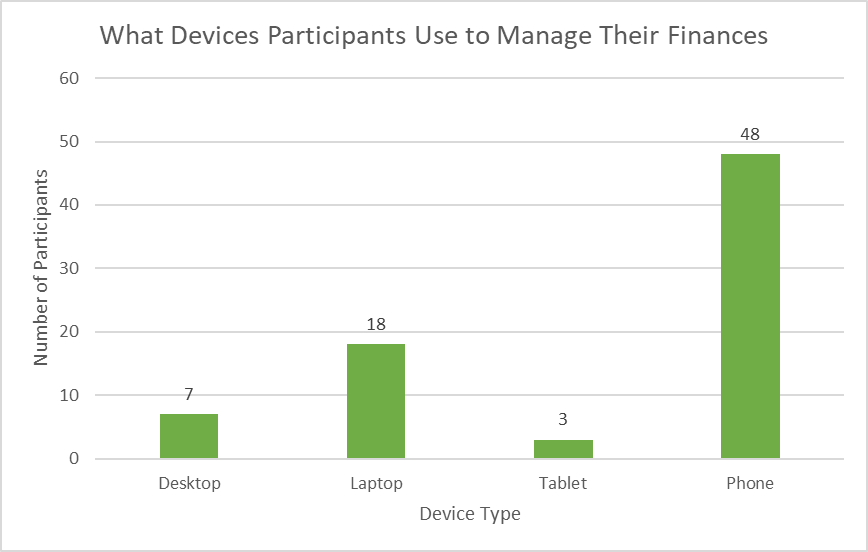
\includegraphics[width=0.5\linewidth]{images/User-Survey/user-survey-charts-devices.png}
    \caption{The types of devices respondents use to manage their finances.}
    \label{fig:devices-main}
\end{figure}

Users typically manage their budgets on a weekly (36\%) or monthly (43\%) basis, so the app should prioritise these reporting periods to align with users’ existing habits. The ability to toggle between these timeframes would also support flexibility for different budgeting styles.

Many respondents still rely on spreadsheets (32\%) or pen and paper (29\%), largely due to their simplicity, flexibility, and the control they offer (see Figure \ref{fig:methods-main}). This reinforces the importance of making the app intuitive and customisable while avoiding the rigidity that discourages users from switching to digital solutions.

\begin{figure}[H]
    \centering
    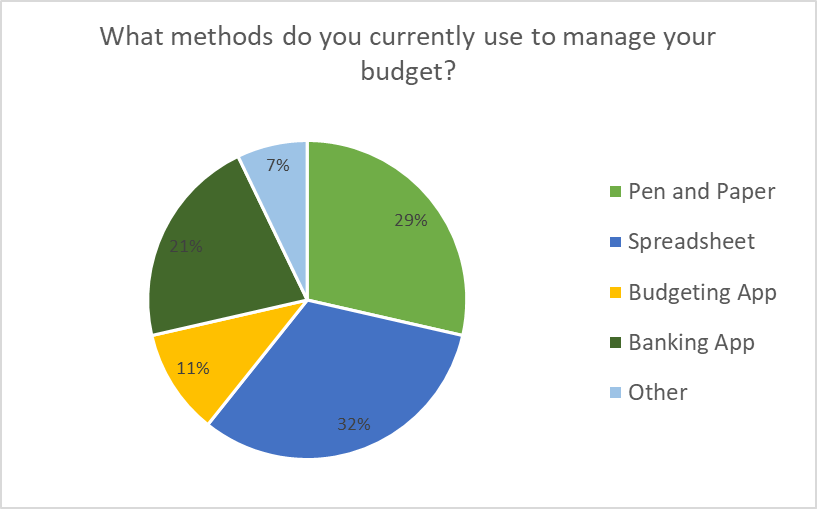
\includegraphics[width=0.5\linewidth]{images/User-Survey/user-survey-charts-methods.png}
    \caption{Chart showing the different tools and methods respondents use to budget.}
    \label{fig:methods-main}
\end{figure}

Only 11\% of participants currently use a budgeting app, with the main reasons for avoiding them being a lack of awareness (44\%), preference for existing methods (35\%), and a perception that budgeting apps are too complex or stressful (17\%). Despite this, 92\% of respondents said they would either consider or be open to trying a budgeting app in the future, showing strong potential demand for an approachable and helpful solution.

The most requested features included:

\begin{itemize}
    \item Spending and income tracking
    \item Categorisation of expenses (e.g. “money pots” or envelope-style budgeting)
    \item Charts and reports to visualise spending habits
    \item Savings goal tracking
    \item Notifications and alerts for limits, bills, and weekly summaries
\end{itemize}

These should form the foundation of the minimum viable product (MVP), especially as they were ranked as the most important by users. Additional suggestions such as banking integration, educational budgeting tips, and customisable reports were also mentioned but may be better suited as future enhancements.

Ease of use is especially important, as many users found existing apps too complicated or overwhelming. Several respondents who do not currently budget said the process felt like too much effort or that they were unsure where to begin. However, many also indicated that the right tool, one that is clear, useful, and simple, would encourage them to start budgeting.

In conclusion, the app should focus on simplicity, flexibility, and usability while delivering core budgeting features. It should also aim to reduce the perceived friction around budgeting, particularly for beginners, by making the experience feel achievable and helpful from the outset.

\section{Initial Requirements}

The following requirements were derived from the initial specification and idea generation session; the comparison of existing budgeting apps; and the user survey. All potential requirements were organised into functional and end-user categories. Functional requirements describe what the system must do to enable user actions, while end-user requirements outline the actions and goals users wish to accomplish \citep{geeksforgeeks_classification_2024}.

\subsection{Functional Requirements}

During early planning, it was discovered that deploying a mobile app through the Google Play Store or Apple App Store required separate developer accounts and various testing and verification processes \citep{google_play_account, apple_developer_account}. Since the aim was to minimise project costs and ensure the application remained easily accessible, it was decided to implement a Progressive Web Application (PWA). A PWA is a web application that can be installed on a user’s device and behaves like a native app \citep{mozilla_progressive_2025}. This mitigated platform-specific concerns, allowed simultaneous development of web and mobile versions, and ensured users could access the app directly through a browser, without relying on an app store.

The resulting functional requirements are as follows:

\begin{itemize}
    \item \textbf{Tech Stack}: React.js frontend, Node.js backend, PostgreSQL database, and deployment via GitHub Pages.
    \item \textbf{System Security and Data Protection}:
    \begin{itemize}
        \item Users must be able to securely log in and access their personal financial data.
        \item Sensitive data, such as passwords, should be protected using secure practices such as hashing before storage.
        \item The system must prevent unauthorised access and comply with data protection principles such as GDPR and the Data Protection Act (DPA).
        \item User data must persist between sessions.
    \end{itemize}
    \item \textbf{Database Requirements}:
    \begin{itemize}
        \item A relational database (PostgreSQL) will be used to store user financial data.
        \item Key entities include: User, Transaction, Bank Account, Category, and Budget.
        \item The database must support full CRUD operations and maintain appropriate relationships between entities.
    \end{itemize}
    \item \textbf{Persistent Storage}: User data must be stored securely on the server and persist between sessions.
    \item \textbf{Device Support}: The application must be optimised for both mobile and desktop use, with responsive UI components to ensure usability across screen sizes.
    \item \textbf{Automatic Categorisation}: Transactions should be categorised based on their name or shop, using rule-based logic or optionally enhanced with machine learning.
\end{itemize}


\subsection{End-User Requirements}
Users should be able to:
\begin{itemize}[noitemsep, topsep=0pt]
    \item Securely log in and manage multiple bank accounts
    \item Add, edit, delete, and repeat income, expense, and savings transactions
    \item Set budget limits by category and receive alerts when overspending occurs
    \item Manage and track savings goals:
    \begin{itemize}
        \item Identify categories to reduce spending on in the next month
        \item See increases in specific expenses over time (e.g. rising electricity bills)
        \item Set specific savings targets (e.g. save £200 this month)
        \item Receive reminders and prompts related to savings goals
    \end{itemize}
    \item Generate financial reports based on:
    \begin{itemize}
        \item Transaction categories, shops, bank accounts, or transaction types
        \item Comparisons between two different time periods (e.g. this month vs the previous month)
        \item Time periods such as daily, weekly, monthly, pay-check to pay-check, or yearly
    \end{itemize}
    \item Filter/sort transactions by date, type, category, shop, or bank account
    \item Search transactions by name or keyword
    \item Export transaction reports and data as PDF or Excel files
\end{itemize}


\section{MoSCoW Prioritisation \& the Minimal Viable Product (MVP)}

MoSCoW prioritisation is a method of organising requirements into categories based on their importance and feasibility \citep{productplan_moscow_nodate}. The categories are:

\begin{itemize}
    \item \textbf{Must Have}: essential product features required for a usable MVP
    \item \textbf{Should Have}: important, but not vital for MVP, but still add significant value
    \item \textbf{Could Have}: features that can improve user experience but have minimal effect if left out
    \item \textbf{Won’t Have}: features that were considered but excluded from this version
\end{itemize}

This method was applied to categorise the initial requirements, from the most essential features to the least critical ones.



\subsection{The Must Haves \& The MVP}

The MVP is made up of all the Must Have requirements, which are listed below:

\begin{itemize}
    \item The user should be able to:
    \begin{itemize}
        \item Securely login to retrieve their data and be confident others cannot view their sensitive financial data
        \item Set their default currency when setting up their account
        \item Log their spending and income with appropriate detail
        \item Edit/delete any of their transactions (with specific options for handling repeated transactions)
        \item View reports/charts on their finances (e.g. pie charts for categories, line graphs for trends) in weekly, monthly, and yearly periods
        \item Set and track budgets and savings goals
        \item Check if they have enough funds to pay bills/upcoming expenses
        \item Clearly see if they have overspent on a category
        \item Receive a notification or alert if they overspend on their overall budget
    \end{itemize}
    \item The app should have persistent storage of the users data even after they leave the app
    \item The application should be mobile friendly and have PWA capability
\end{itemize}

\subsection{The Should \& Could Haves}

These features would be included in the MVP if time permits, but they were deprioritised to non-essential for the initial version of the app.

\vspace{0.5em}
\textbf{Should Have}
\vspace{0.5em} \\
The user should be able to:
\begin{itemize}
    \item Set the currency of each transaction
    \item Create custom categories
    \item Create and track multiple bank accounts
    \item Edit/delete their bank accounts
    \item View additional chart types (e.g, spending per shop)
    \item View charts in additional reporting periods (e.g. fortnightly)
    \item Generate bank-account specific reports
    \item Set concrete savings goals e.g. put £200 away in a savings account this month
    \item Make use of advanced transaction filtering and sorting
\end{itemize}

\vspace{0.5em}
\textbf{Could Have}
\vspace{0.5em} \\
The user could:
\begin{itemize}
    \item Convert transactions in currencies different from their default currency into their default currency using current exchange rates
    \item Log repeated transactions where the payment amount may change each time
    \item View charts in additional time periods (daily, pay-day-to-pay-day)
    \item Export reports (PDF, Excel)
    \item Search transactions by name
    \item Generate cash flow visualisations
    \item View suggestions on which categories they should reduce spending
    \item Receive notifications when their bills increase
    \item Attach interest rates to their bank accounts so that they can view how much interest each account is earning
\end{itemize}

\subsection{The Won’t Haves}
This version of the application will not include:
\begin{itemize}
    \item Automatic categorisation of transactions
    \item Bank account integration
\end{itemize}

\begin{figure}[H]
    \centering
    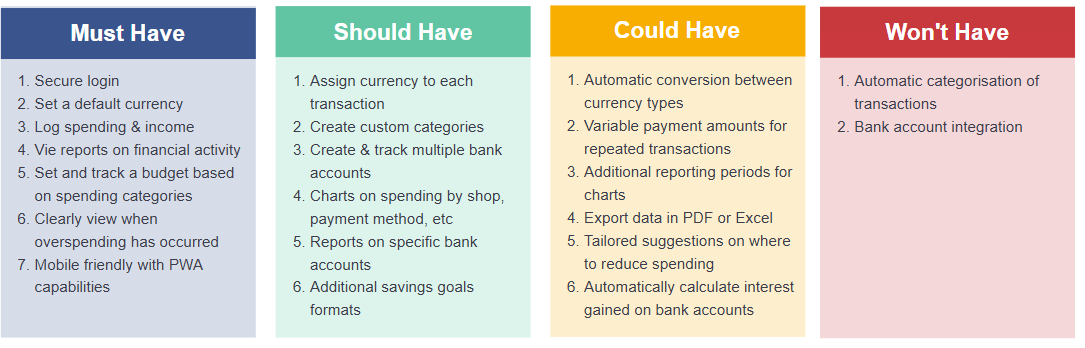
\includegraphics[width=\linewidth]{images/moscow.png}
    \caption{Summarised MoSCoW prioritisation}
    \label{fig:moscow}
\end{figure}


%==================================================================================================================================
\chapter{Design}
\section{Architecture Design}
\subsection{Initial Design}
The initial architecture was designed as a web application using the React.js framework for the frontend, a Node.js server for middleware, and a PostgreSQL database for backend storage. The frontend was also intended to include Progressive Web App (PWA) capabilities. This setup supported the goals of creating a system that was scalable, accessible, and cost-effective to deploy across multiple platforms.

React was selected as it is one of the most widely adopted JavaScript libraries for building dynamic and responsive UIs. Its large developer community, comprehensive documentation, and reusable component structure make it a strong choice for rapid development \citep{komodo_9_2022}. The component-based architecture also promotes clear separation of concerns and simplifies long-term UI maintenance.

The decision to use a PWA aimed to improve accessibility and usability, especially on mobile devices. PWAs combine aspects of web and native apps, allowing users to install the application directly onto their devices without an app store \citep{mozilla_progressive_2025}. This reduces friction for users and avoids the overhead of maintaining separate iOS and Android apps.

Node.js was chosen for the backend due to its strong performance with asynchronous operations and seamless integration with JavaScript-based frontends like React. It is lightweight, efficient, and well-suited for building RESTful APIs \citep{geeksforgeeks_pros_2024}.

PostgreSQL was selected as the database system for its robust relational capabilities, support for complex queries, and strong data integrity via its ACID-compliant architecture. It integrates well with Node.js through tools like node-postgres and supports advanced data types and indexing \citep{postgresql_about, npm_pg_2025}.

\subsection{Final Design}
Before development began, the frontend framework was switched from React to Angular. The primary motivation was Angular’s more structured setup, which simplified project management and scaling as the application became more complex.

A key advantage of Angular is its built-in support for features such as routing, form validation, and state management which are critical for a financial system handling significant volumes of user data. In contrast, React would have required third-party libraries to achieve similar functionality. Angular also offers native PWA support, streamlining the addition of offline and installable capabilities compared to React’s more manual configuration \citep{sakthi_unlocking_2024}.

The decision was further influenced by prior industry experience using Angular in a financial dashboard project, which also required strict data validation, modularity, and security. This background provided greater confidence in using Angular to build a reliable and secure system.

Angular is commonly adopted in enterprise applications, especially those handling sensitive data. It promotes best practices such as strong typing through TypeScript, automatic protection against common vulnerabilities, and a consistent project structure. Its use in platforms like PayPal demonstrates its suitability for financial applications \citep{sols_angular_nodate}.

The final system architecture is shown in Figure~\ref{fig:architecture}, and initial sketches of both the React and Angular versions can be found in Appendix~\ref{app:architecture}.

\begin{figure}[htb] 
    \centering
    \begin{subfigure}[b]{\textwidth}
        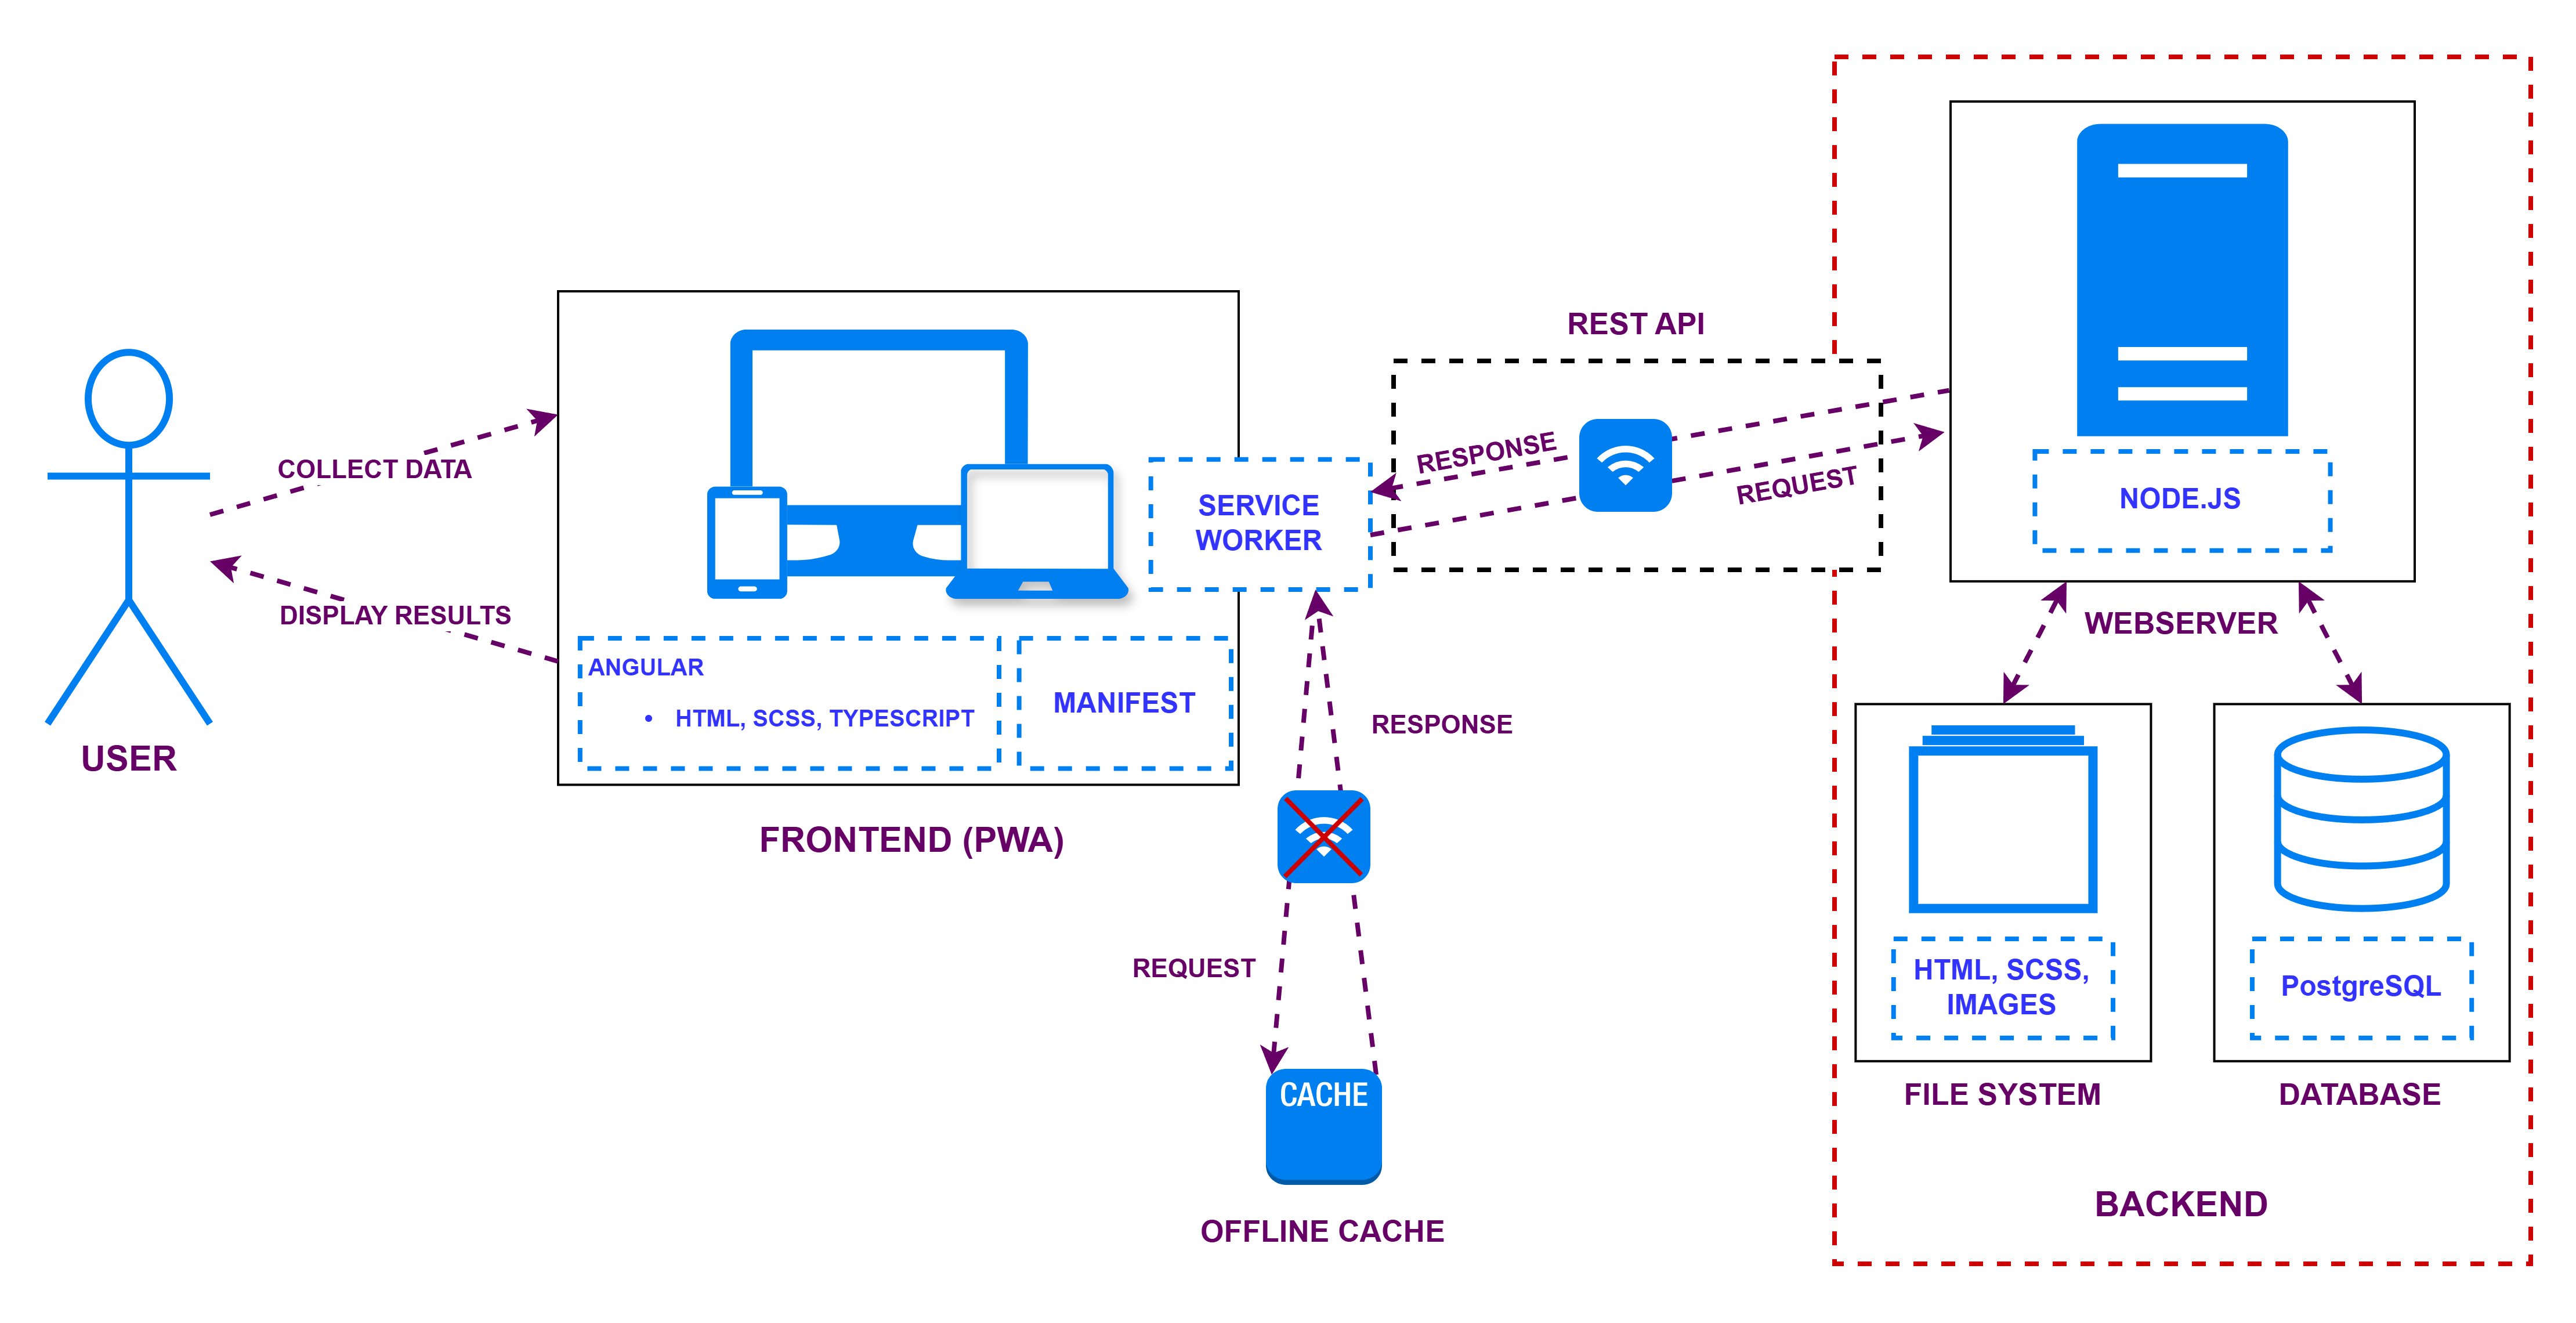
\includegraphics[width=\textwidth]{images/Architecture-Diagrams/final-architecture-diagram.png}
        \label{fig:syn1}
    \end{subfigure}   
    \caption{Final architecture design using an Angular front-end with the PWA labelled. \\ \\
    \textbf{Service Worker} - manages offline access, push notifications and caching of the PWA. \\
    \textbf{Manifest} - enables installable app on mobile and desktop.}
    \label{fig:architecture}
\end{figure}


\section{Database Design}
\subsection{Data Types \& Storage Considerations}
When designing the database schema, a number of informed decisions were made about the data types used and the structure of the entities.

Adherence to normalisation principles was important for reducing redundancy and dependency between records and fields. This was particularly important given the likelihood of strict storage constraints from a free hosting service, so space needed to be used efficiently. This focus on normalisation also helps to maintain data integrity, as it enforces constraints and relationships between entities. The theory outlined in \citet{elmasri_fundamentals_2017} \textit{Fundamentals of Database Systems} was followed, which resulted in the schema being in Boyce-Codd Normal Form (BCNF). This means that all inherent dependencies are removed, and each attribute in the entities is dependent only on its associated primary key. BCNF is considered the industry-standard level of normalisation that database designers strive to achieve, representing that the schema has been broken down into efficient and well-structured relations. Although these methods are often used to improve existing databases, the definition of BCNF was used to guide the design from the beginning, keeping in mind normalisation principles such as reducing null values, avoiding duplicate information, and ensuring that properties are only dependent on their necessary primary key.

The emphasis of data normalisation on reducing redundancy, along with the awareness of storage space limitations, led to the decision to not store calculated or intermediate values such as the user’s current bank balance, category totals, total amount spent, and so on. Instead, it was planned for this responsibility to be handled by the front-end. While this approach may result in higher levels of processing and potentially impact performance, it allows more users to enter additional transactions and other financial data within the available storage constraints.

Security and compliance with data protection laws remained a priority throughout the design process, and it was established that user passwords would need to be hashed and stored securely. While hashing alone provides some protection against data breaches, the addition of a randomised salt to the hashing of users’ passwords makes it significantly more difficult for attackers to use tools such as rainbow tables or offline dictionary attacks to access user accounts if the password data were compromised. Salts are important because they prevent duplicate passwords from being recognised or mixed up within the relation, and also help protect users who may reuse passwords across different systems from being identified \citep{salomon_2018}.

Research and consideration were given to selecting appropriate data types for key fields. The serial data type was chosen for primary key IDs in each entity as this allows for up to 2 billion unique values that are automatically incremented. As this is a small-scale project, the assumption was made that none of the entities would ever contain more than 2 billion entries. For currency fields, guidance from \citet{crunchydata_working_postgres} was followed, allowing for 9 digits, with 2 of those reserved for decimal places. Only two decimal places were used, as intermediate or calculated values were not stored, so further precision was not necessary. This choice allows money values up to 9,999,999.99, which should be more than sufficient for users using the app to manage their real-life finances.


\subsection{MVP Database}
Using the considerations mentioned earlier, the schema for the MVP was developed as shown in Figure \ref{fig:mvp-database}. The data type decisions made for each property are outlined in Table \ref{tab:mvp-database-table}.

The User entity stores login credentials, the user's default transaction currency, and their starting bank account balance upon sign-up. The Category entity stores fixed values for the different transaction and budgeting categories and cannot be edited by users. The Transaction entity holds all information about the user’s transactions, including whether a particular transaction is recurring. The Budget table includes each category in the user's budget alongside the limit they have set for that category. Finally, the Savings\_Goal entity stores the user’s goal amount, their target date for reaching it, and how much they have saved towards that goal when creating it.

\begin{figure}[htb] 
    \centering
    \begin{subfigure}[b]{0.75\textwidth}
        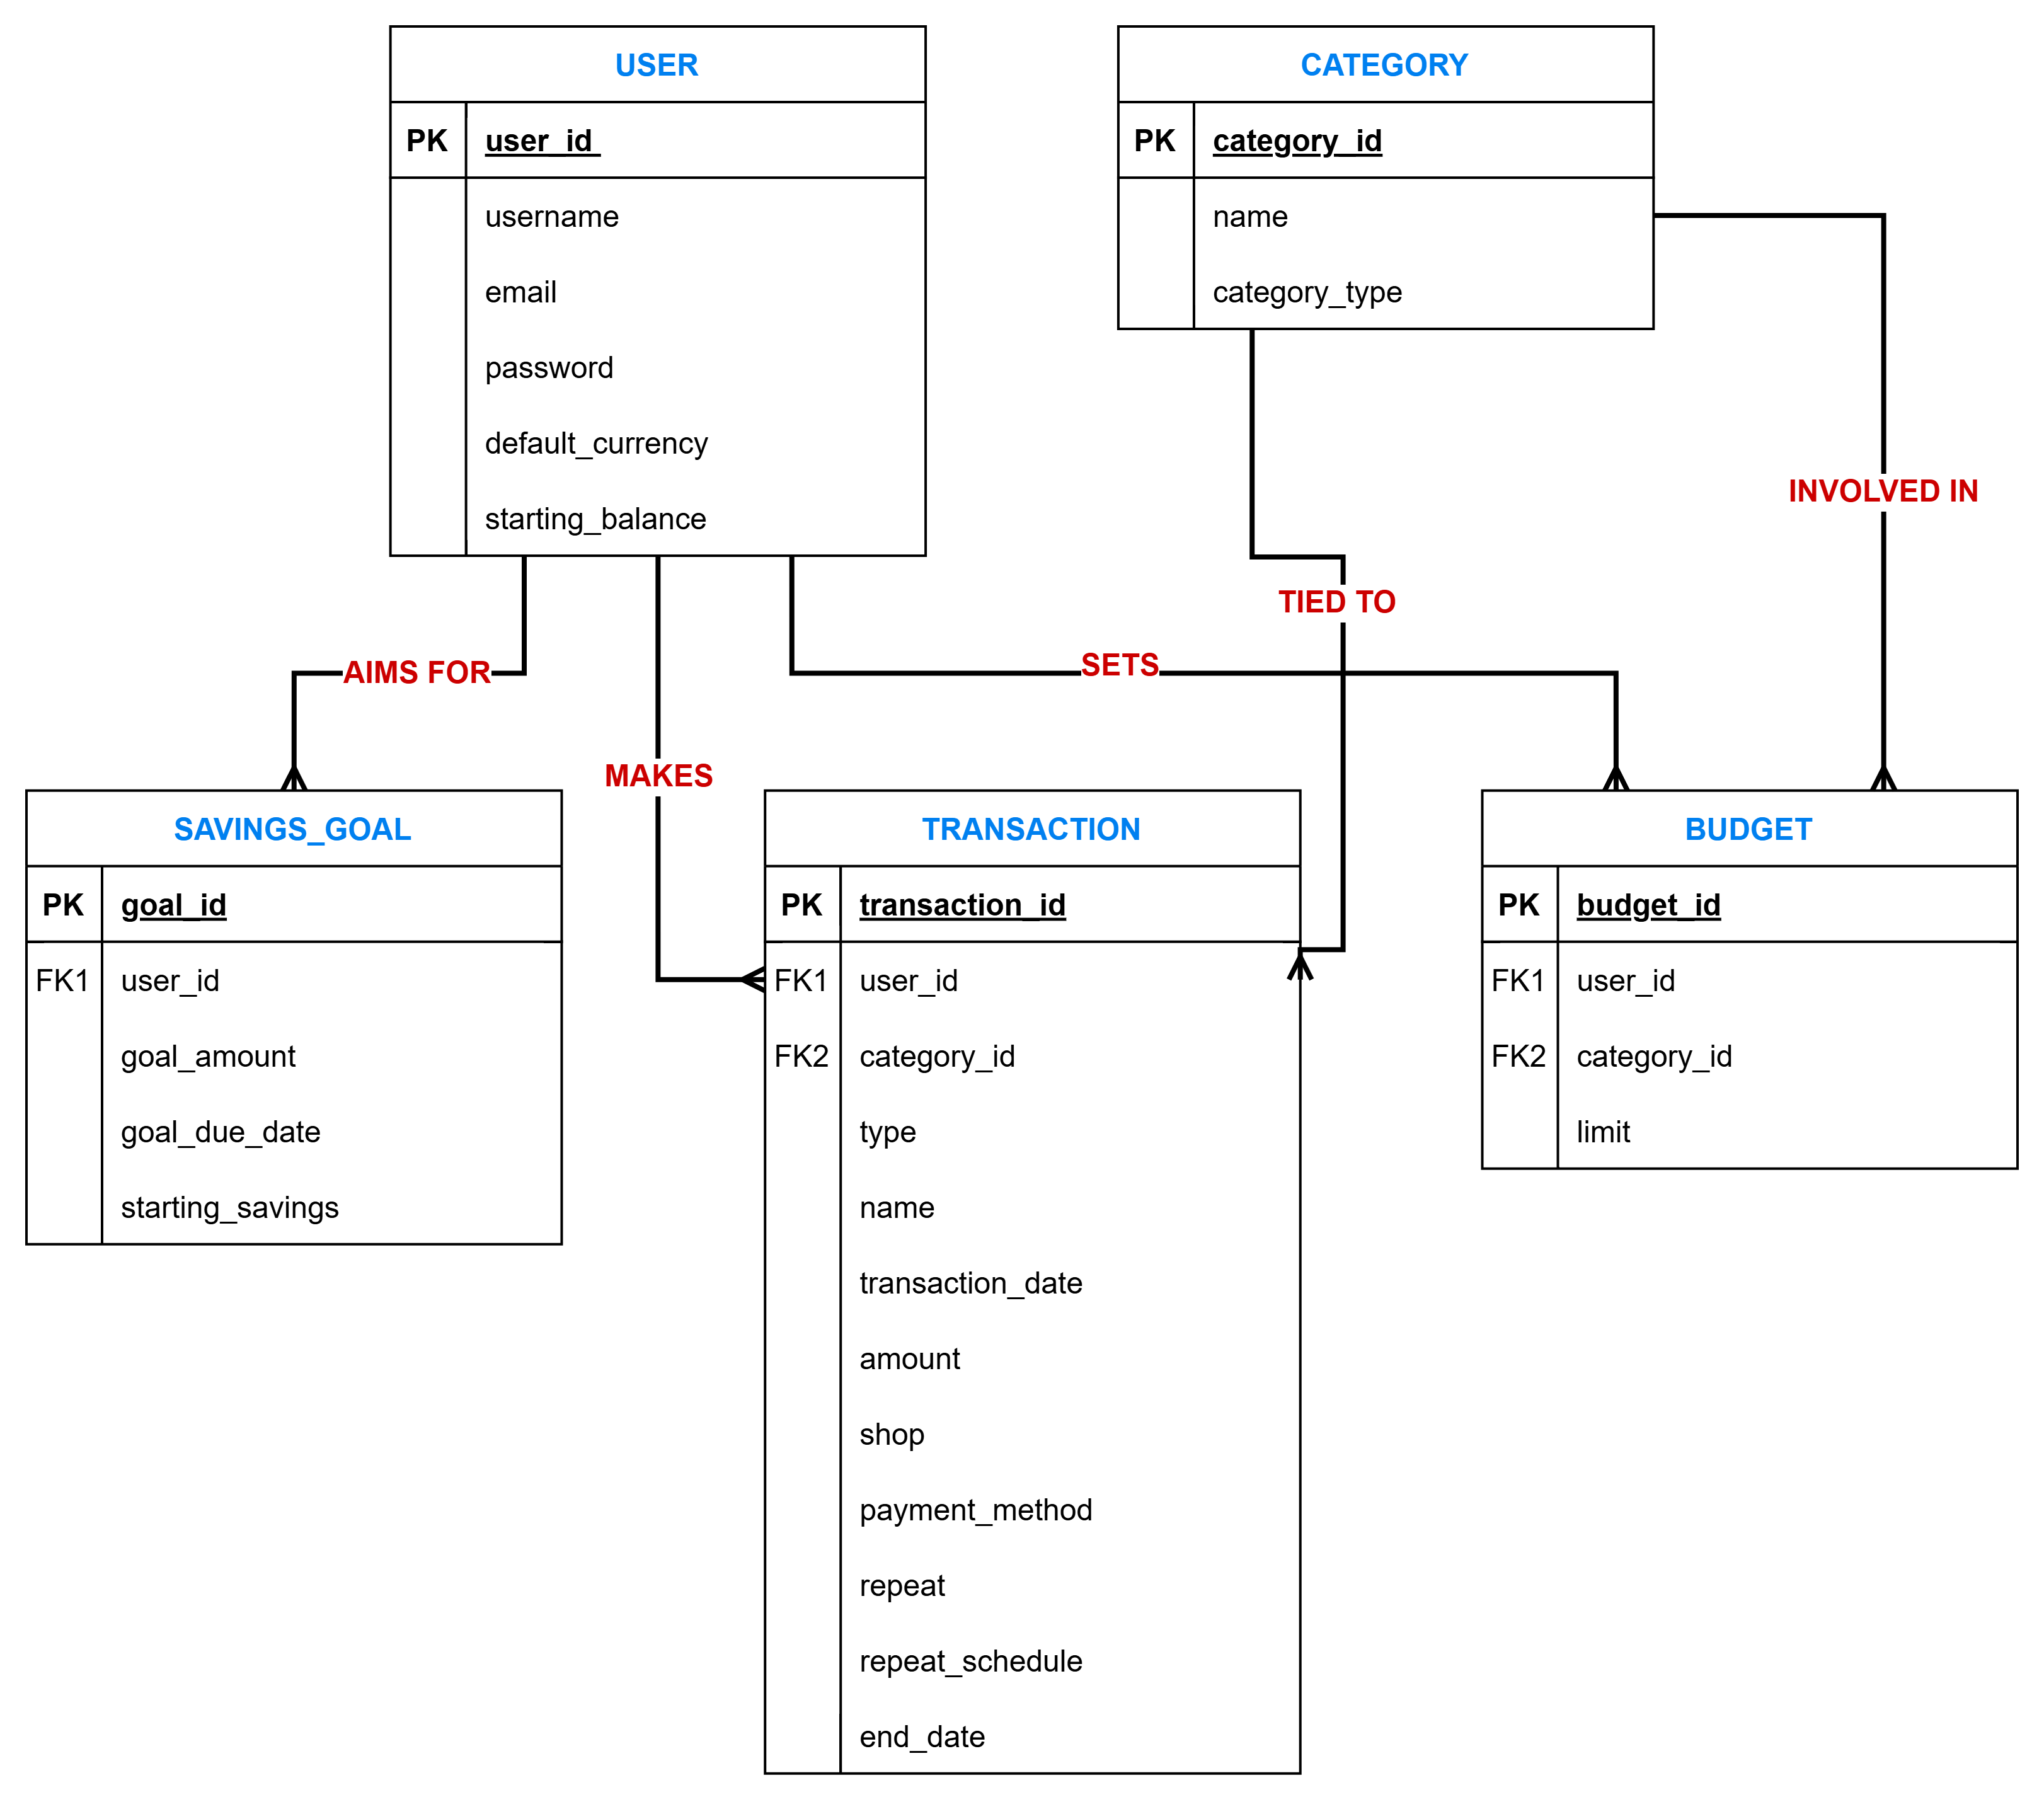
\includegraphics[width=\textwidth]{images/ER-Diagrams/final_MVP_ER.png}
        \label{fig:syn1}
    \end{subfigure}   
    \caption{ER diagram for the MVP. "PK" and underlines indicate primary keys and "FK" indicates foreign keys.}\label{fig:mvp-database}
\end{figure}


\begin{table}[htb]
    \centering
    \caption{MVP Property Table}
    \label{tab:mvp-database-table}
    \begin{adjustbox}{max width=\textwidth,center}
    \small
    \begin{tabular}{|l|l|l|l|l|}
        \hline
        \textbf{Entity} & \textbf{Property} & \textbf{Data Type} & \textbf{Constraints} & \textbf{Other} \\
        \hline
        USER & user\_id & serial & PK & \\
        USER & username & varchar(30) & Unique, Not Null & \\
        USER & email & varchar(255) & Unique, Not Null, Valid Email Format & \\
        USER & password & varchar(255) & Not Null, Encrypted with a Salt & \\
        USER & default\_currency & varchar(3) & Not Null, in ISO 4217 Currency Codes format & \\
        USER & starting\_balance & numeric(9,2) & Not Null, default to 0.00 & \\
        CATEGORY & category\_id & serial & PK & \\
        CATEGORY & name & varchar(255) & Not Null & \\
        CATEGORY & category\_type & enum(‘expense’, ‘income’, ‘savings’) & Not Null & \\
        SAVINGS\_GOAL & goal\_id & serial & PK & \\
        SAVINGS\_GOAL & user\_id & serial & Not Null & FK \\
        SAVINGS\_GOAL & goal\_amount & numeric(9,2) & Not Null & \\
        SAVINGS\_GOAL & goal\_due\_date & datetime & Not Null & \\
        SAVINGS\_GOAL & starting\_savings & numeric(9,2) & Not Null, default to 0.00 & \\
        TRANSACTION & transaction\_id & serial & PK & \\
        TRANSACTION & user\_id & serial & Not Null & FK \\
        TRANSACTION & category\_id & serial & Not Null & FK \\
        TRANSACTION & type & enum(‘expense’, ‘income’, ‘savings’) & Not Null & \\
        TRANSACTION & name & varchar(255) & Not Null & \\
        TRANSACTION & transaction\_date & datetime & Not Null & \\
        TRANSACTION & amount & numeric(9,2) & Not Null & \\
        TRANSACTION & shop & varchar(255) & & \\
        TRANSACTION & payment\_method & enum(‘credit’, ‘debit’, ‘cheque’, ‘cash’) & & \\
        TRANSACTION & repeat & Boolean & Default to False & \\
        TRANSACTION & repeat\_schedule & enum(‘daily’, ‘weekly’, ‘monthly’, ‘yearly’) & Default to Null & \\
        TRANSACTION & end\_date & datetime & Default to Null & \\
        BUDGET & budget\_id & serial & PK & \\
        BUDGET & user\_id & serial & Not Null & FK \\
        BUDGET & category\_id & serial & Not Null & FK \\
        BUDGET & limit & numeric(9,2) & Not Null & \\
        \hline
    \end{tabular}
    \end{adjustbox}
\end{table}
\normalsize
\newpage


\subsection{Should Have \& Could Have Databases}
Schemas for the Should Have and Could Have requirements were also designed to ensure that, if these features were implemented, the necessary database structures would already be available.

Figure \ref{fig:non-mvp-er-diagrams} shows both the Should Have and Could Have ER diagrams, with changes from the MVP highlighted in yellow. The new or updated properties are summarised in Table \ref{fig:non-mvp-tables}.

The additions in the Should Have schema are as follows:
\begin{itemize}
    \item A new Bank\_Account entity, allowing users to track multiple bank accounts
    \item A user\_id property added to the Category entity, enabling users to create custom categories
    \begin{itemize}
        \item This property would be set to null for the default categories available to all users
    \end{itemize}
    \item A currency property added to the Transaction entity, so users can specify if a payment was made in a different currency than their default
    \item A bank\_account\_id property added to the Transaction entity, so users can indicate which of their bank accounts the transaction relates to
\end{itemize}
\vspace{0.5em}
The further enhancements shown in the Could Have schema include:
\begin{itemize}
    \item A variable\_value property in the Transaction entity, indicating whether a repeated transaction may have different amounts each time
    \item A notes\_and\_tags property in the Transaction entity, allowing users to include additional details or tags about the transaction
    \item A spend\_less property in the Budget entity, which indicates that the user wants to reduce spending in that category
    \item An interest\_rate property in the Bank\_Account entity, allowing the app to calculate and display the interest earned for each account.
\end{itemize}

\begin{figure}[htb]
    \centering
    \begin{subfigure}[b]{1\textwidth}
        \caption{Should Have Property Table - New and modified properties since the MVP.}
        \tiny
        \begin{adjustbox}{max width=\textwidth,center}
        \begin{tabular}{|l|l|l|l|l|}
            \hline
            \textbf{Entity} & \textbf{Property} & \textbf{Data Type} & \textbf{Constraints} & \textbf{Other} \\
            \hline
            CATEGORY & user\_id & serial & Optional & FK \\
            TRANSACTION & bank\_account\_id & serial & Not Null & FK \\
            TRANSACTION & currency & numeric(9,2) & Not Null, default to the user default\_currency & \\
            BANK\_ACCOUNT & bank\_account\_id & serial & & PK \\
            BANK\_ACCOUNT & user\_id & serial & Not Null & FK \\
            BANK\_ACCOUNT & name & varchar(255) & Not Null & \\
            BANK\_ACCOUNT & starting\_balance & numeric(9,2) & Not Null, defaults to 0.00 & \\
            BANK\_ACCOUNT & account\_type & enum(‘savings’, ‘current’, ‘joint’, ‘ISA’) & Not Null & \\
            \hline
        \end{tabular}
        \end{adjustbox}
        \label{fig:syn1}
    \end{subfigure}
    \begin{subfigure}[b]{1\textwidth}
        \caption{Could Have Property Table - Additional potential enhancements beyond Should Have.}
        \tiny
        \begin{adjustbox}{max width=\textwidth,center}
        \begin{tabular}{|l|l|l|l|l|}
            \hline
            \textbf{Entity} & \textbf{Property} & \textbf{Data Type} & \textbf{Constraints} & \textbf{Other} \\
            \hline
            TRANSACTION & variable\_value & Boolean & Default to False & \\
            TRANSACTION & notes\_and\_tags & varchar(500) & Optional & \\
            BUDGET & spend\_less & Boolean & Defaults to False & \\
            BUDGET & end\_date & datetime & Default to Null & \\
            BANK\_ACCOUNT & interest\_rate & decimal(5,4) & Not Null, default to 0.0000 & \\
            \hline
        \end{tabular}
        \end{adjustbox}
        \label{fig:syn2}
    \end{subfigure}

    \caption{New and modified properties introduced since the MVP. The Should Have table lists essential changes, while the Could Have table includes optional enhancements.}
    \label{fig:non-mvp-tables}
\end{figure}
\normalsize

\begin{figure}[htb] 
    \centering
    \begin{subfigure}[b]{0.45\textwidth}
        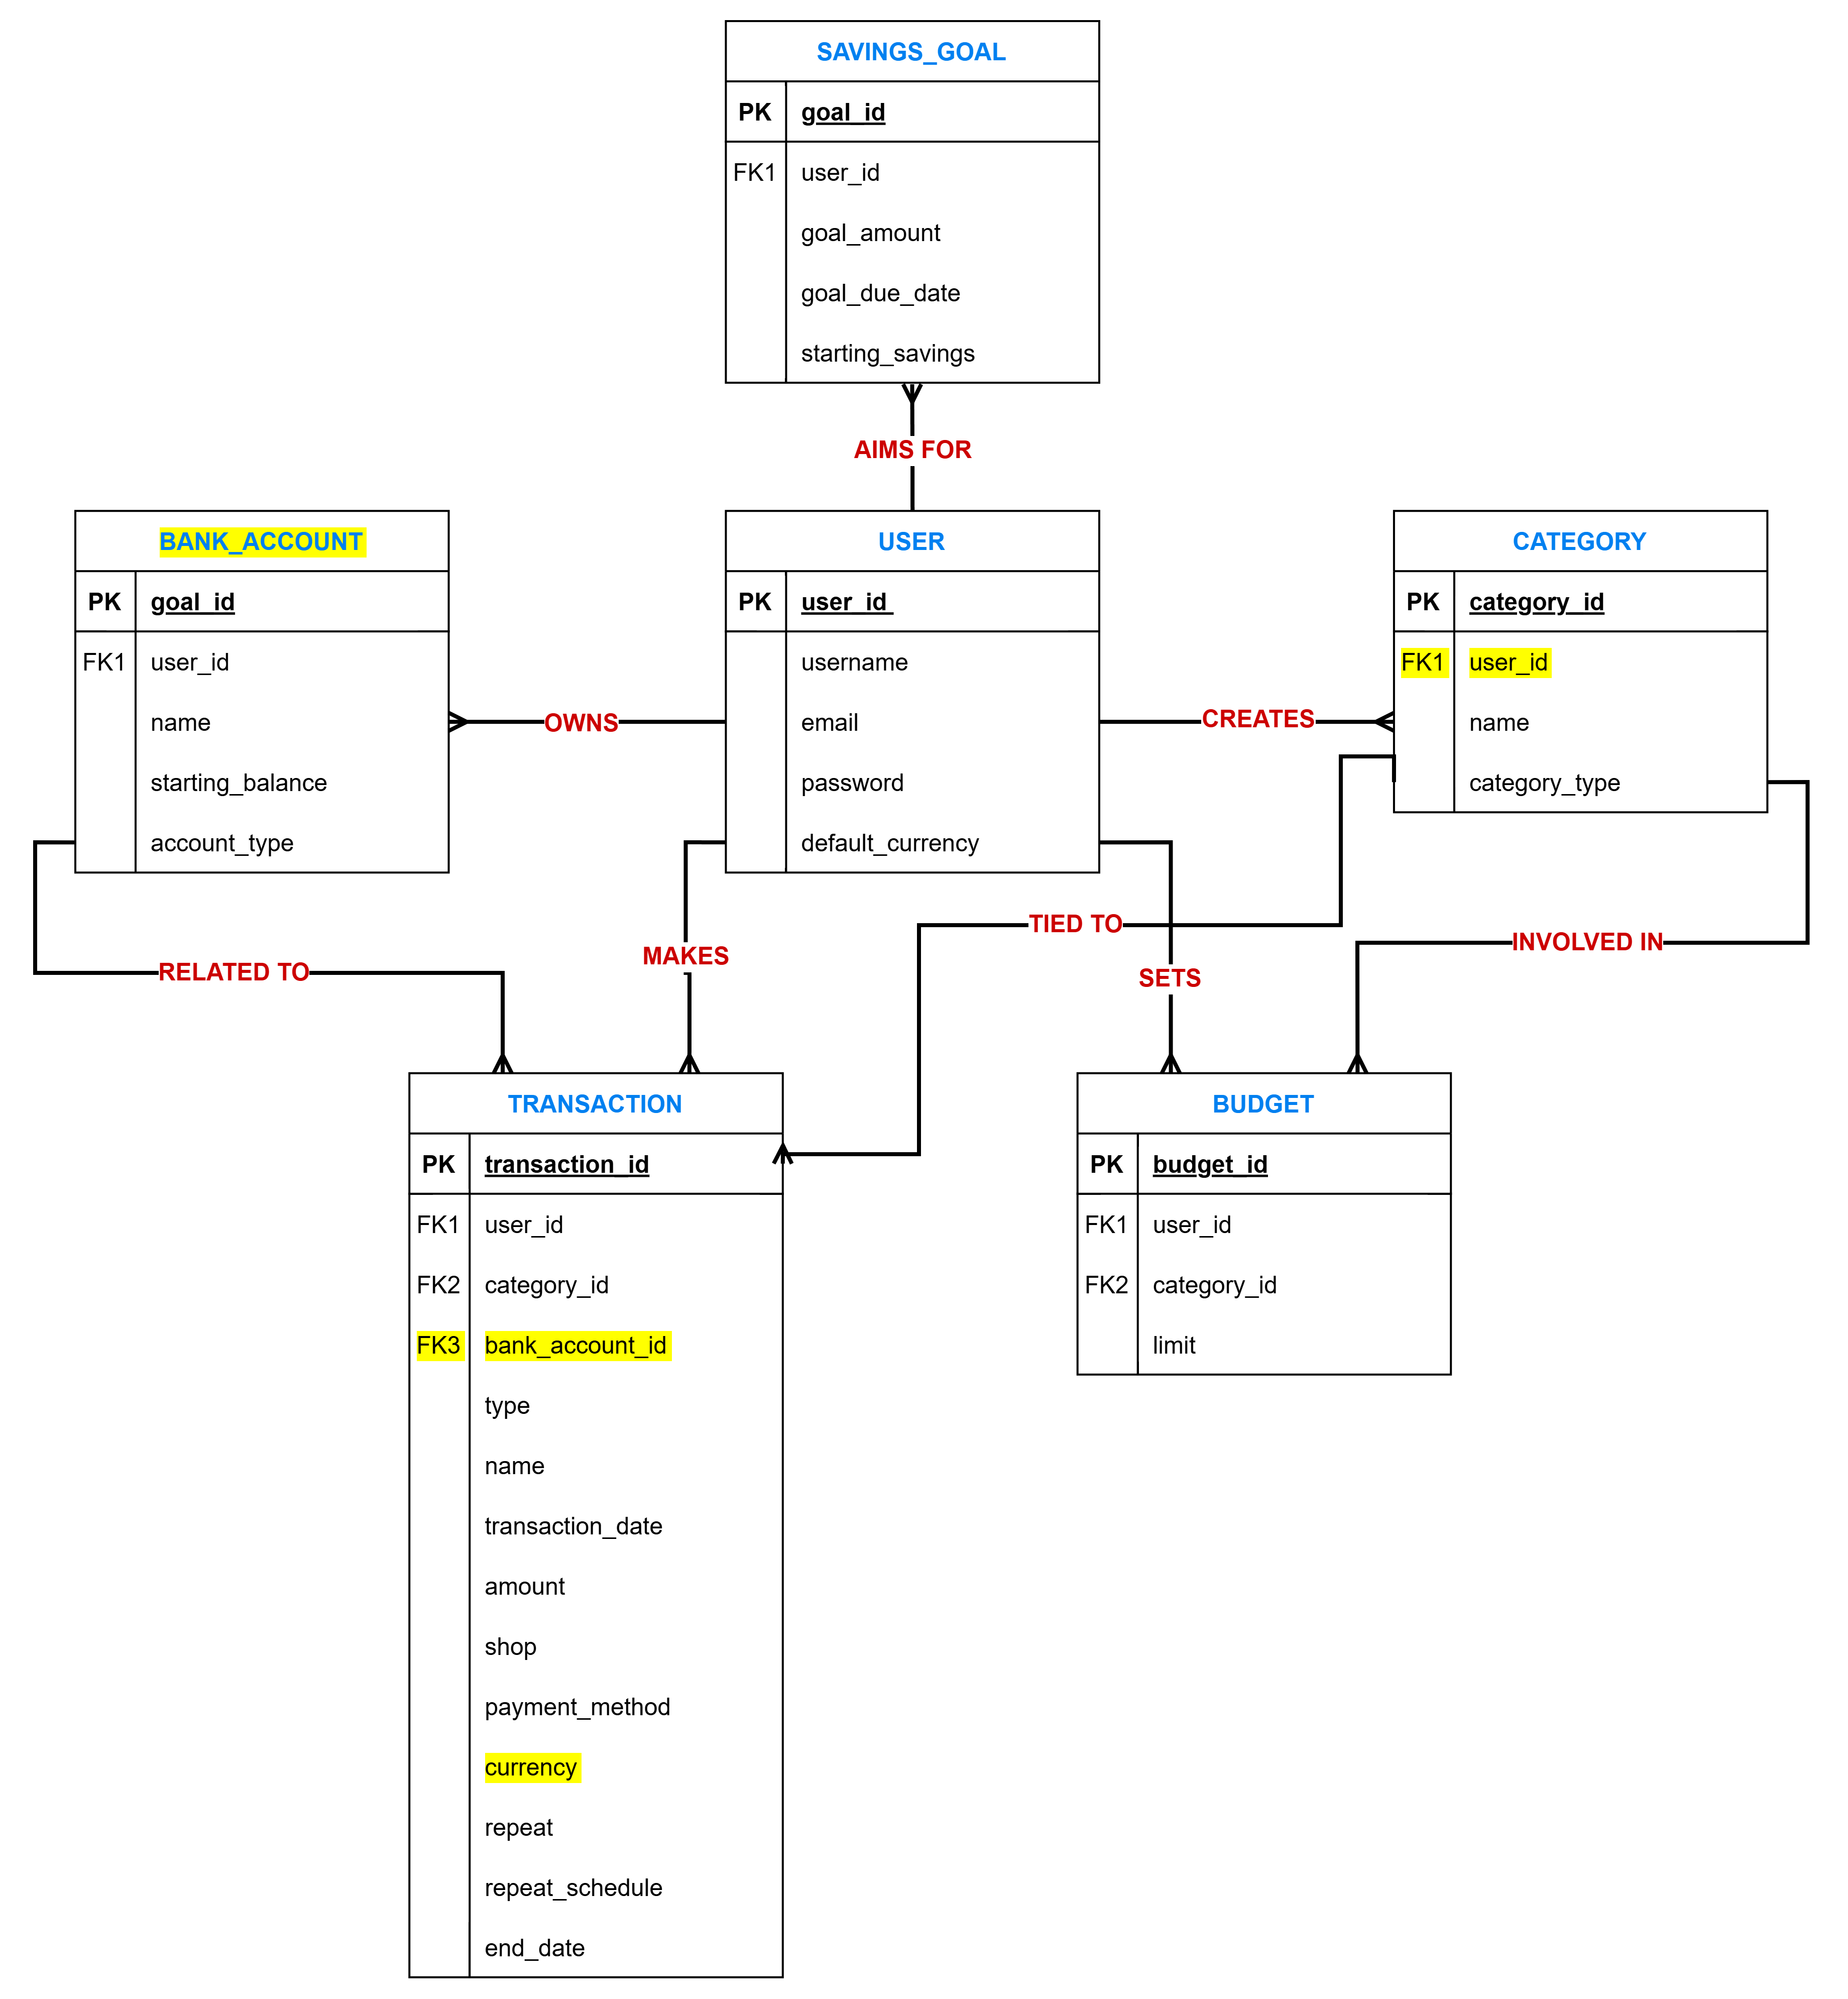
\includegraphics[width=\textwidth]{images/ER-Diagrams/final_should_have_ER.png}
        \caption{Should Have ER Diagram.}
        \label{fig:syn1}
    \end{subfigure}
    \begin{subfigure}[b]{0.45\textwidth}
        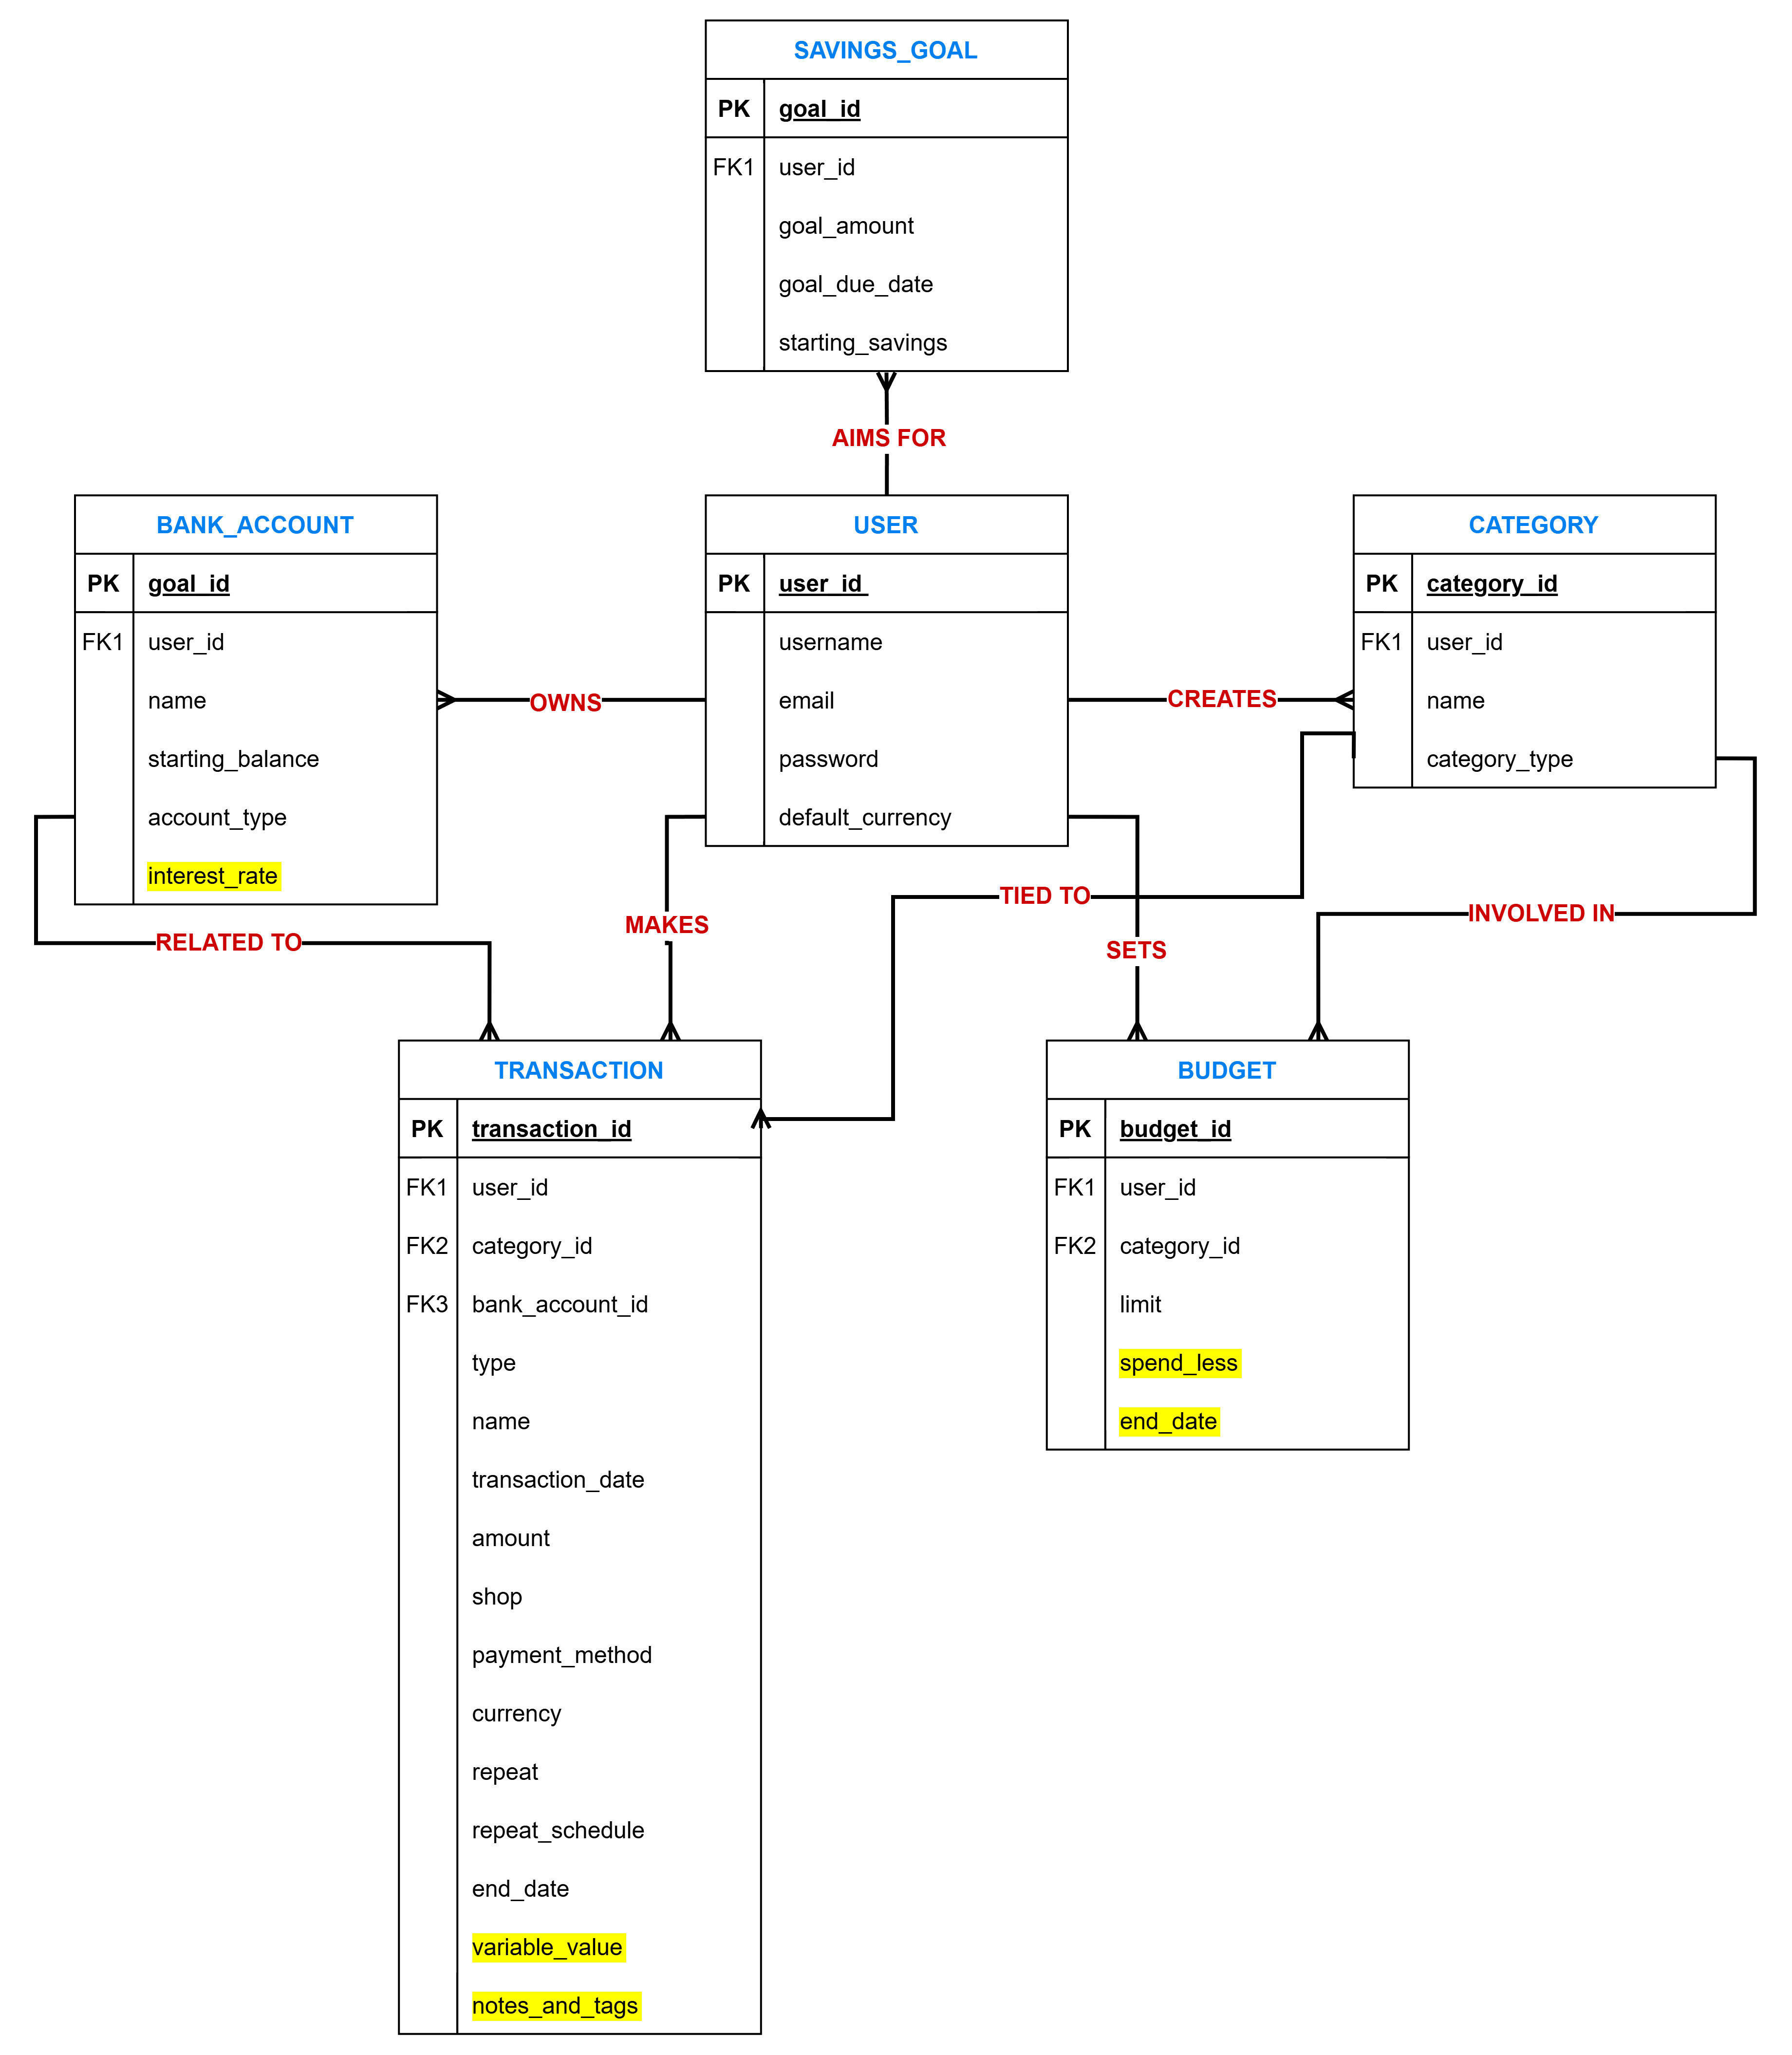
\includegraphics[width=\textwidth]{images/ER-Diagrams/final_could_have_ER.png} 
        \caption{Could Have ER Diagram.}
        \label{fig:syn2}
    \end{subfigure}   
    \caption{Yellow highlights show the changes from the previous ER diagram. I.e. highlights in the Should Have diagram are changes from the MVP and highlights in the Could Have diagram are changes from the Should Have.
    }\label{fig:non-mvp-er-diagrams}
\end{figure}
\newpage


\section{UI Design}
\subsection{Wireframes}
Since the application was going to be developed as a web app but also needed to be mobile-friendly, wireframes were designed for each page in both phone and desktop formats. An example of these two layouts can be seen in Figure \ref{fig:wireframes-home}.

\begin{figure}[H] 
    \centering
    \begin{subfigure}[b]{0.6\textwidth}
        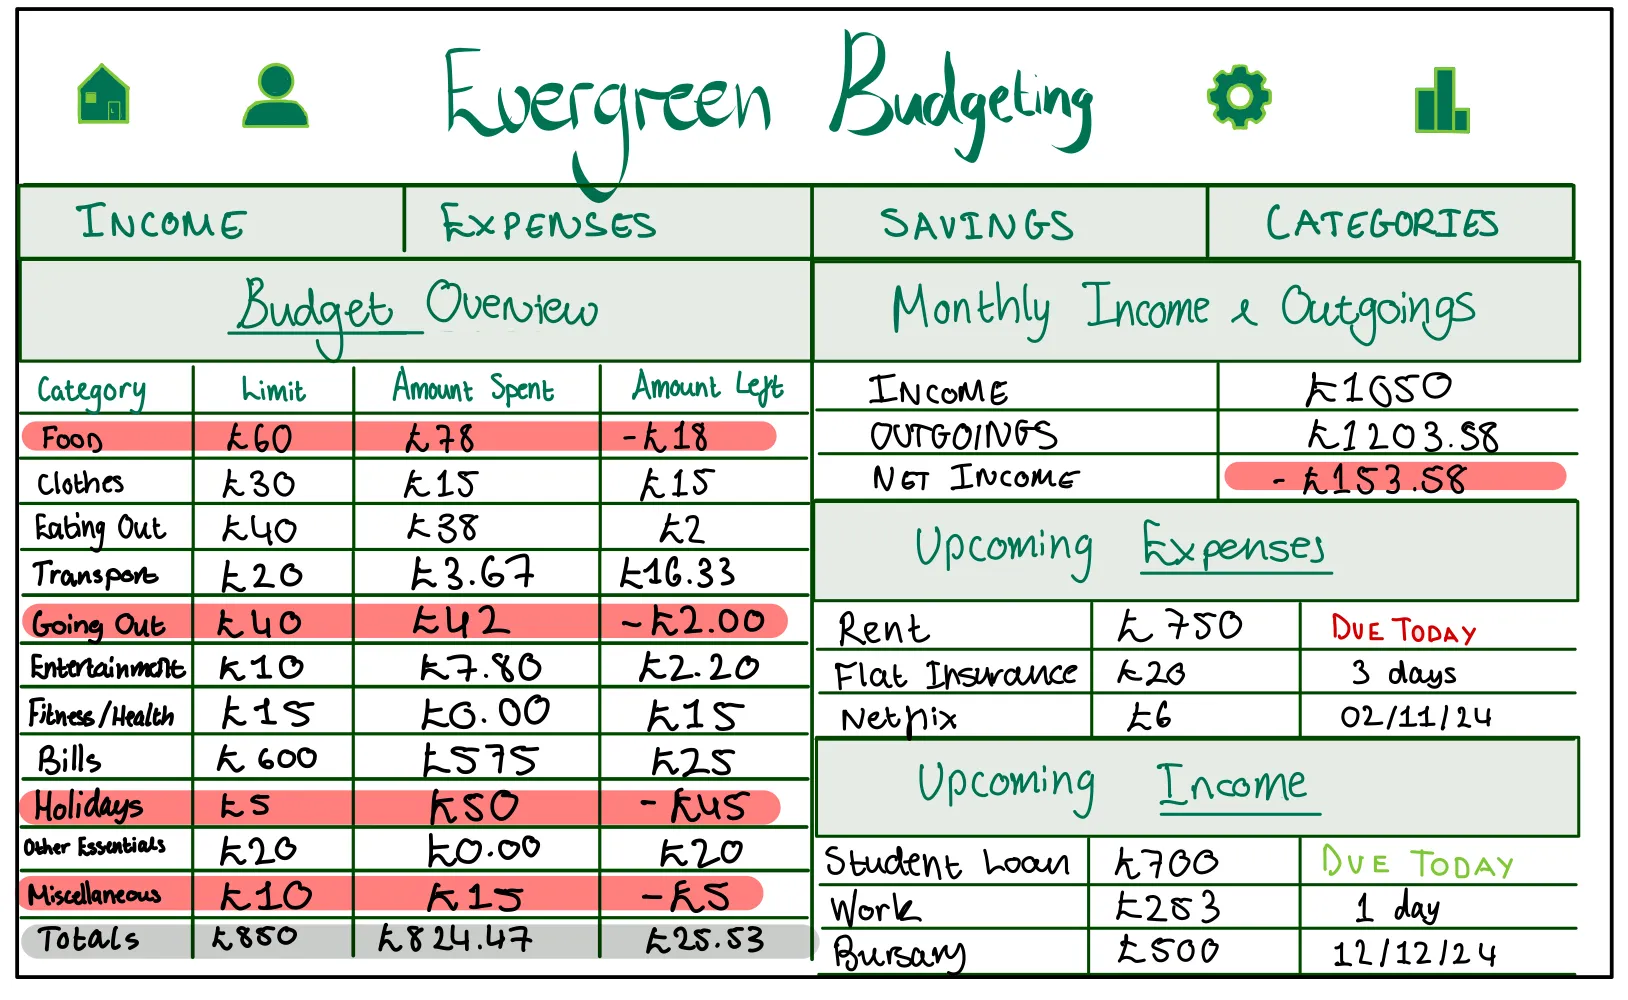
\includegraphics[width=\textwidth]{images/Wireframes/wireframe-home-desktop.png}
        \caption{Desktop View}
        \label{fig:syn1}
    \end{subfigure}
    ~
    \begin{subfigure}[b]{0.28\textwidth}
        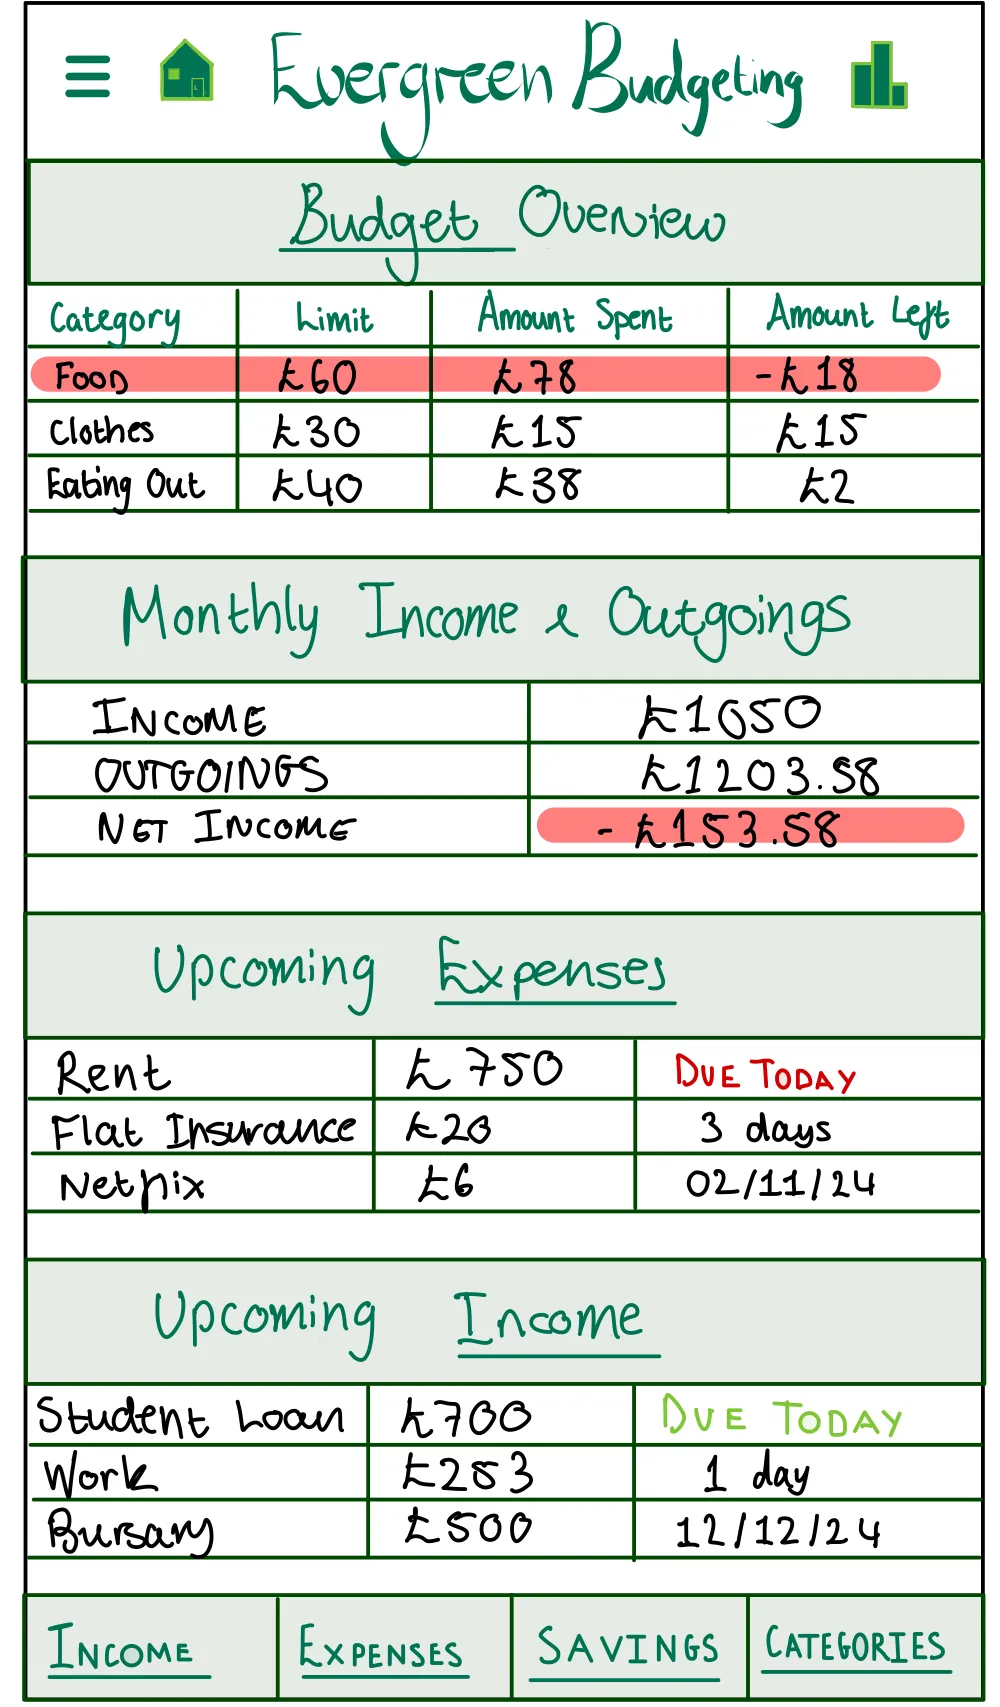
\includegraphics[width=\textwidth]{images/Wireframes/wireframe-home-phone.png} 
        \caption{Phone View}
        \label{fig:syn2}
    \end{subfigure}
    \caption{Wireframes for the app's home page.}
    \label{fig:wireframes-home}
\end{figure}
\newpage

Before designing the look and feel of the UI, a name for the app was needed. A soothing and calming concept was chosen based on feedback from the user study, which highlighted that one barrier to using budgeting apps is that users can find them overwhelming. This led to a nature-themed concept.

The idea of "money trees" was considered initially, but this felt a bit too obvious. Eventually, the name Evergreen Budgeting was selected, a title that maintained the nature theme while subtly referencing the money tree idea. The word evergreen also evokes a sense of longevity and financial stability, as evergreen trees retain their leaves year-round. Additionally, green is commonly associated with money, making the name feel both relevant and approachable.

Once the name was chosen, the app's aesthetic and colour palette were tailored to suit it, with many elements adopting a green or nature-inspired look. A clean and minimal interface was still prioritised, as many potential users expressed a preference for simplicity and ease of use.

For displaying data, a table-based approach was chosen. The user survey indicated that spreadsheets are a popular budgeting tool, so this design choice aimed to mimic a familiar and preferred format for users. These tables are shown in Figure \ref{fig:wireframe-income}.

\begin{figure}[htb] 
    \centering
    \begin{subfigure}[b]{0.6\textwidth}
        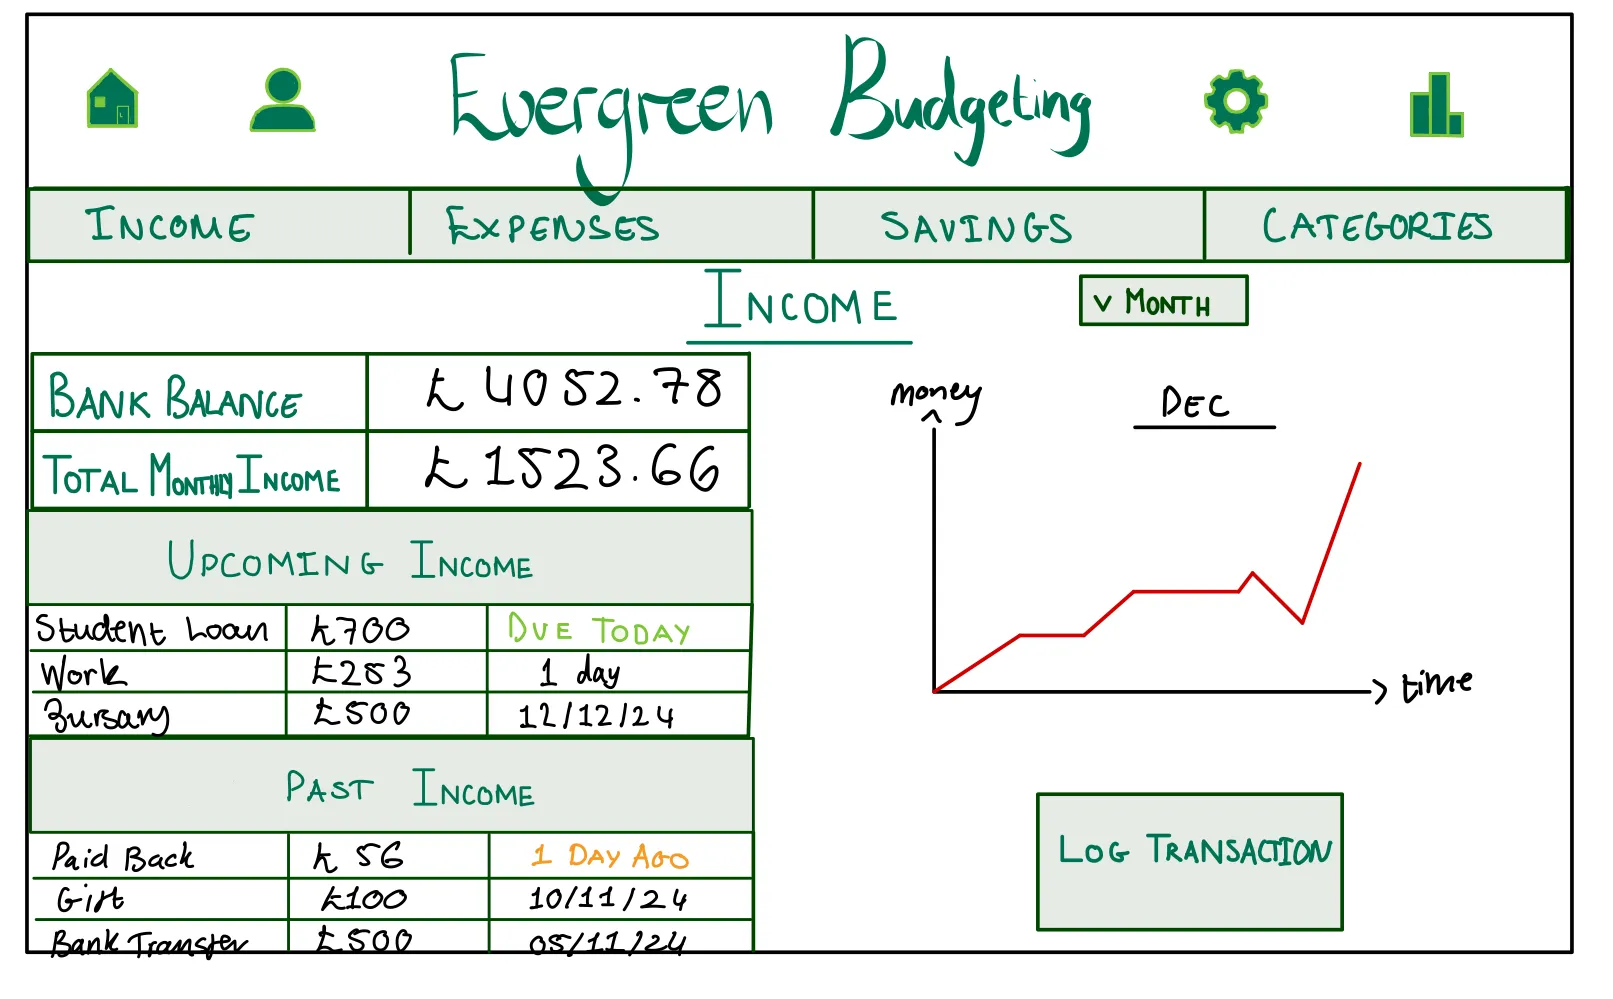
\includegraphics[width=\textwidth]{images/Wireframes/wireframe-income-desktop.png}
    \end{subfigure}   
    \caption{Wireframe for the income page.}
    \label{fig:wireframe-income}
\end{figure}

For the reports page, the intention was to allow users to view multiple financial reports, each highlighting different aspects of their finances (see Figure \ref{fig:wireframe-reports}). The charts were also designed to be customisable, allowing users to filter the data by time period and transaction type. Three charts were included:

\begin{enumerate}
    \item A pie chart showing a breakdown of transactions by category. Users can toggle between expense, income, and savings categories, and select the time period they want to view.
    \item A line chart showing income, expenses, and net balance over the chosen time period.
    \item A bar chart displaying total spending across different time units (e.g. monthly totals for the past year).
\end{enumerate}
\vspace{0.5em}

\begin{figure}[htb] 
    \centering
    \begin{subfigure}[b]{0.6\textwidth}
        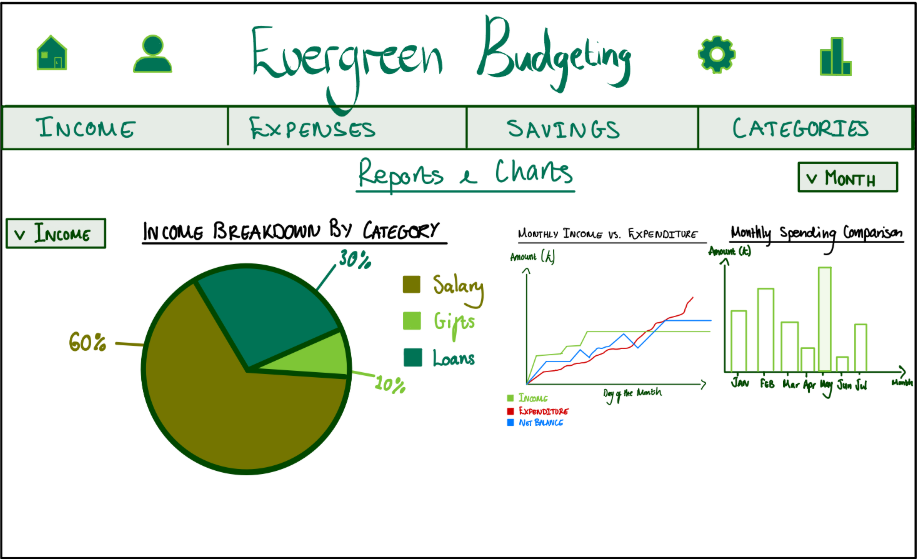
\includegraphics[width=\textwidth]{images/Wireframes/wireframe-reports-desktop.png}
    \end{subfigure}   
    \caption{Wireframe for the reports page.}
    \label{fig:wireframe-reports}
\end{figure}

For the budget page (Figure \ref{fig:wireframe-budget}), a more visual and engaging approach was used rather than another table. In keeping with the nature theme, watering cans were designed to act as progress bars for each category in the user’s budget. If a user overspends in a category, the watering can overflows and is highlighted in red to clearly indicate this.

\begin{figure}[htb] 
    \centering
    \begin{subfigure}[b]{0.6\textwidth}
        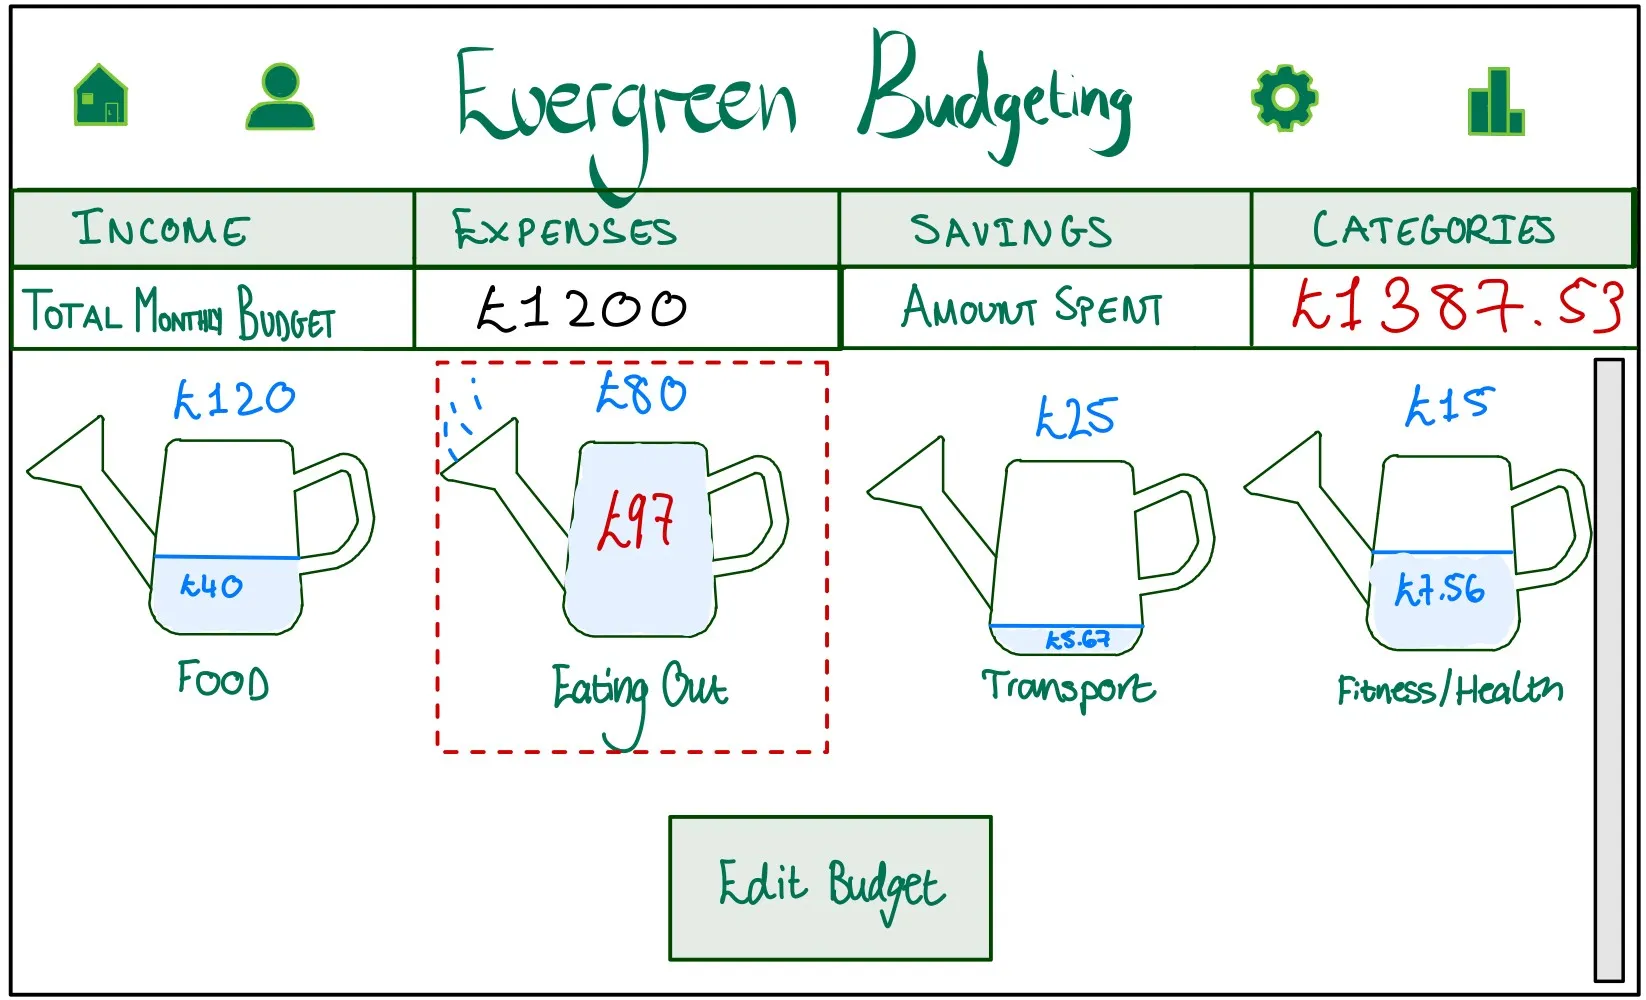
\includegraphics[width=\textwidth]{images/Wireframes/wireframe-budget-desktop.png}
    \end{subfigure}   
    \caption{Wireframe for the budget page.}
    \label{fig:wireframe-budget}
\end{figure}

Wireframes for the remaining pages (both phone and desktop views) can be found in Appendix \ref{app:wireframes}.

\subsection{Logo}
Time was also spent designing the logo for the application, following the wireframe stage, as a distinctive icon was needed for users’ home screens. The process began by looking at logos from other budgeting apps and various tree-inspired designs. The aim was to steer away from money imagery and instead focus on themes of tracking and reporting, while still tying in with nature.

The final logo (Figure \ref{fig:logo}) reflects the app’s overall colour palette and aesthetic. The tree trunk and main structure are styled to resemble a bar chart, subtly tying in the financial tracking theme. Logo inspirations can be found in Appendix \ref{app:logo-inspiration}.

\begin{figure}[htb] 
    \centering
    \begin{subfigure}[b]{0.25\textwidth}
        
\includegraphics[width=\textwidth]{images/Logo/logo.png}
    \end{subfigure}   
    \caption{The logo for Evergreen Budgeting.}\label{fig:logo}
\end{figure}

\section{Design Changes}
\subsection{Database Changes}
During implementation, a number of changes were made to the initial database design as it became clearer what worked in practice and what did not. Some of these were smaller adjustments, for example:

\begin{itemize}
    \item The limit attribute in the Budget entity had to be renamed, since “limit” is a reserved keyword in PostgreSQL.
    \item The user ID and category ID in the Budget entity were combined to create a composite key.
    \begin{itemize}
        \item This ensures that a user cannot have duplicate budget categories in their budget.
    \end{itemize}
    \item The data type for all money-related fields was changed to numeric(20,2), allowing for much larger values.
    \begin{itemize}
        \item Originally, only nine digits had been allocated, but currencies where values are typically much higher, even for low purchasing power, had not been considered.
    \end{itemize}
\end{itemize}

\vspace{0.5em}
In addition to these minor tweaks, more structural changes were also made:

\begin{itemize}
    \item A goal\_name field was added to the Savings\_Goal entity, allowing users to assign meaningful names to each of their goals.
    \item A ranking attribute was introduced in the Savings\_Goal entity to allow users to prioritise their savings goals.
    \begin{itemize}
        \item With this ranking system, a user's available savings are distributed in order of priority, starting with the top-ranked goal, and any surplus then trickling down to the next goals in the list.
    \end{itemize}
\end{itemize}

\vspace{0.5em}
Another key addition was the repeat\_group\_id field in the Transaction entity. This is used to link together transactions that are part of a recurring schedule. For instance, if a user logs a transaction that repeats on the 1st of every month from 01/01/2025 to 01/12/2025, the system will automatically generate 12 transactions with the same details but different dates. Each of these transactions is tagged with a shared repeat\_group\_id, making it easy to identify and manage all transactions within that group, such as when editing or deleting all future instances of that recurring transaction.

\subsection{Navigation Bar Redesign}
Some time was also spent during implementation redesigning the navigation bar. Initially, the original design was implemented, but it quickly became apparent that there would not be a profile or settings page at this stage, and that many key pages, such as the budget and transaction pages, were inaccessible through the nav bar.

Because of this, the design was updated so that the logo, home, transaction, budget, and report pages were visible and accessible from all pages, allowing for easier navigation. Since the income, expense, and savings pages shared a similar layout and functionality, they were grouped under a single “Transactions” dropdown menu.

The updated navigation bar can be seen in Appendix \ref{app:wireframes-nav-bar}.

The mobile version of the nav bar required fewer changes, as the necessary options were simply added to the hamburger menu. However, the “Evergreen Budgeting” text was replaced with the logo, and the home and reports icons were removed.



%==================================================================================================================================
\chapter{Implementation}
\section{Software Engineering Process}
\subsection{Version Control \& Continuous Integration}

Git and GitHub were selected for version control in order to more easily and efficiently manage changes to the codebase, and to maintain a record of the project's progress.

The project development followed a feature branch workflow. For each major milestone or new feature, a dedicated branch was created, separate from the master branch. This made it easier to work on individual features without introducing instability into the main application. Once a feature was completed, it was then merged back into the master branch.

Commits were made at the end of each coding session, once the code was functional and stable. This helped to ensure that the repository was updated regularly with small, incremental changes. It also provided a record of the development history, which made it easier to identify when and where certain changes were made. Each commit was linked to a relevant GitHub issue, helping to maintain documentation between tasks and code changes.

These version control practices were selected to improve code readability, reduce the risk of integration conflicts, and contribute to a more streamlined and maintainable development process \citep{chacon_straub_git}.

\subsection{Issue Management}
Effective issue management was essential to maintaining focus and organisation throughout the project. Milestones were used to represent major features, while individual tasks and sub-features were tracked as issues within each milestone. 

A Kanban board was implemented using GitHub Projects to track and coordinate these tasks (see Figure \ref{fig:kanban}). The board was structured around four columns: Backlog, To Do, In Progress and Done. The Backlog served as a holding area for tasks not included in the current unit of work, while To Do listed items ready to be started. Issues were moved to Done either after the code’s deployment to production or, for non-code-related tasks, following the addition of an explanatory comment.

Each issue contained key information to assist with planning and execution, including the associated milestone; a detailed summary of the task; a time estimate; and a priority label (see Appendix \ref{app:issues}). Priority was categorised into three levels: low, medium and high. These distinct, yet limited, options allowed for clear distinctions between urgent and lower-priority work. For time estimation, a t-shirt sizing system was used with three options: small, medium and large.  This approach allowed for quick approximation of task complexity, particularly in cases where precise time predictions were difficult, and helped facilitate realistic workload distribution across the development timeline.

\begin{figure}[h]
    \centering
    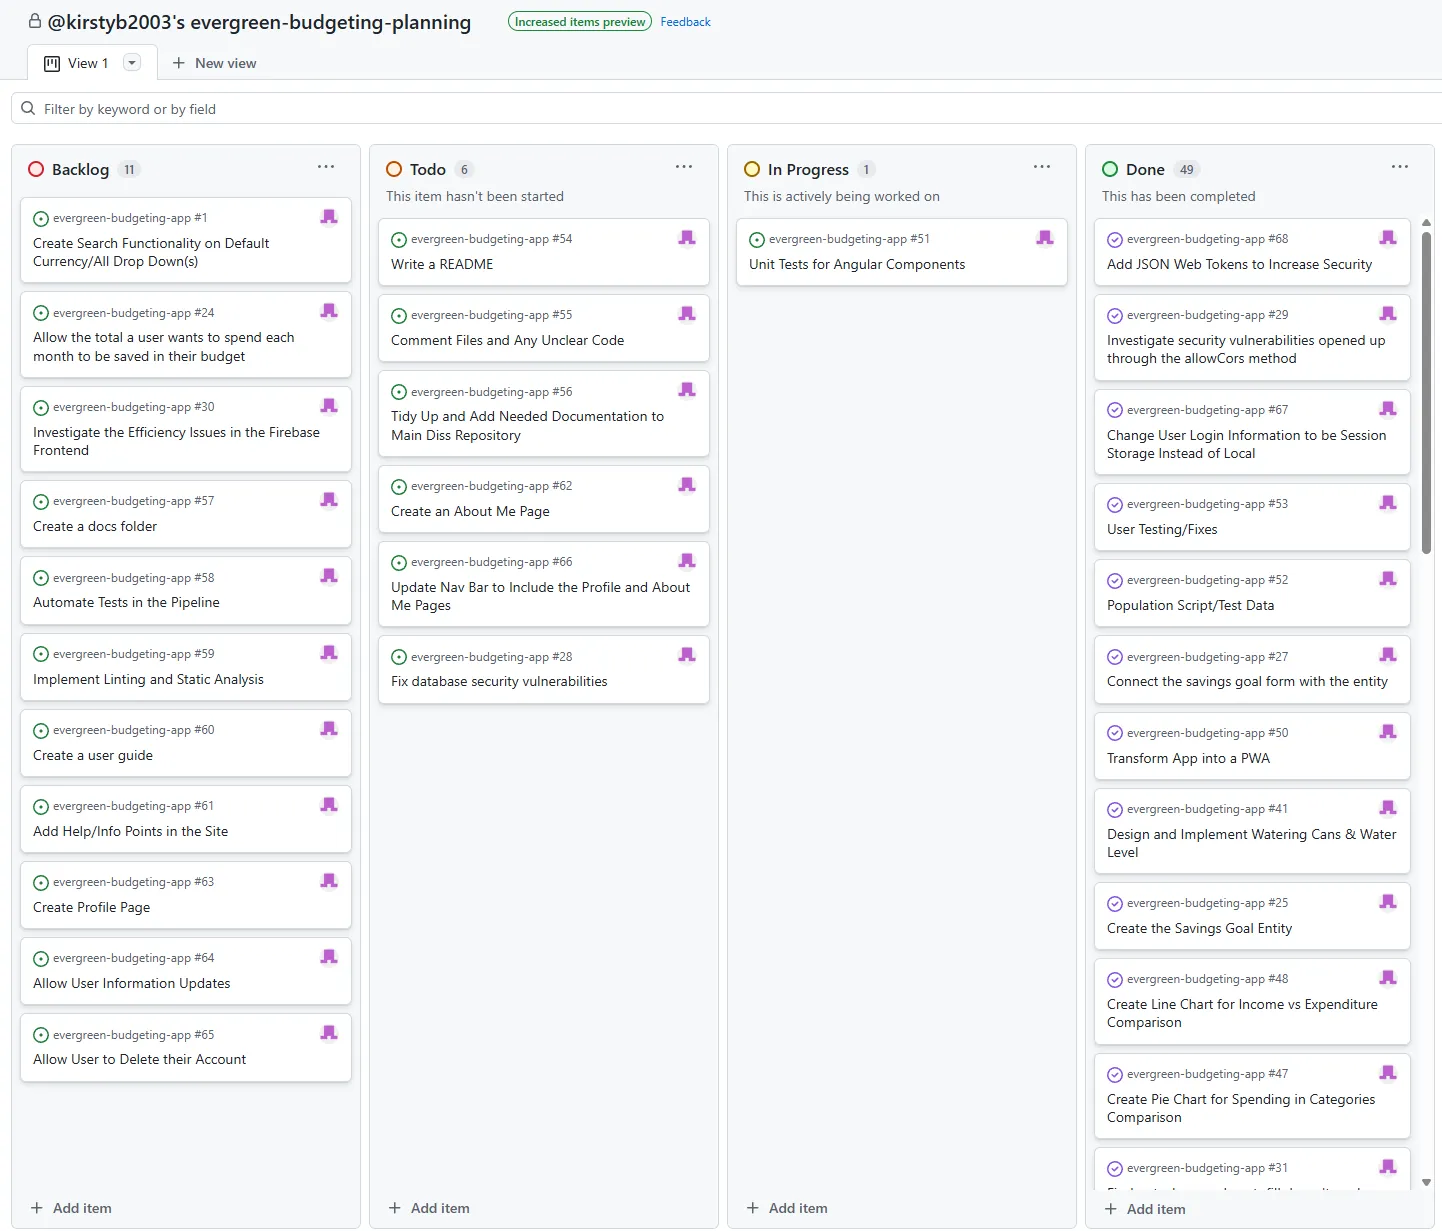
\includegraphics[width=0.75\linewidth]{images/GitHub-Screenshots/kanban-board.png}
    \caption{Kanban board implemented with GitHub Projects}
    \label{fig:kanban}
\end{figure}

\subsection{Continuous Deployment}

The application was continuously deployed using a CI/CD pipeline powered by \citet{github_actions_deploying}. Whenever changes were pushed to the master branch, an automated workflow was triggered to deploy the latest version of the application.

The master branch served as the production branch, and no changes were merged into it until they had been tested and reviewed on their respective feature branches. Once a feature was complete, the branch was merged into master, triggering the deployment pipeline.

Deployment automation was configured using a deploy.yaml file, which outlined the necessary steps for building and deploying both the frontend and backend components. Authentication for deployment was managed using GitHub Secrets to ensure secure and automated access to both of the hosting platforms.

The benefits of continuous deployment strategies are discussed in software engineering literature. \citet{humble_continuous_2010} highlight how automation leads to faster feedback loops, reduced deployment errors, and more reliable software delivery. Similarly, \citet{fowler_continuous_integration} emphasises the importance of CI/CD in streamlining development workflows and enabling rapid, iterative releases.

\section{Features}
This section describes the features successfully implemented and how these related to the initial set of requirements. Further screenshots of the final product can be found in Appendix \ref{app:ui-screenshots}.

\subsection{Login \& Registration}
A key requirement of the MVP was that users should be able to log in securely to access their personal data. This functionality was fully implemented. All pages, other than the login and registration pages, are protected using an Angular AuthGuard, which ensures that only authenticated users can access routes that display sensitive data.

When a user logs in, a JSON Web Token (JWT) is generated by the backend and stored in session storage. This token is used to validate the user’s identity on future requests, preventing unauthorised access to sensitive data. Passwords are securely handled using hashing with a salt before storage. During login, the entered password is hashed and compared server-side within the database query, ensuring plaintext passwords are never exposed. These methods are discussed further in Section \ref{sec:security}.

Another key requirement was allowing users to select a default currency during the registration process. This value is collected via a dropdown input on the registration form, where users choose from a list of currency options represented by their corresponding ISO 4217 currency codes (e.g. GBP, EUR, USD).

\subsection{Setting \& Managing a Budget}
When implementing the “creating a budget” functionality, a number of considerations were taken. First, the approach would involve the categorisation of spending, while also placing emphasis on savings. Second, the design aimed to allow the user to approach their budget setup from different perspectives. As a result, the budget form was implemented with two distinct methods: the user could either build their budget by allocating values to individual spending categories based on expectations or needs, or alternatively, start with a fixed overall budget amount and divide it across categories, with any remaining balance automatically allocated to savings. This flexibility supports both income-focused and spending-focused approaches to financial planning.

Form validation was handled using Angular’s built-in features, with reactive warnings to alert users if they exceeded their total budget (see Figure \ref{fig:budget-form}). In the income-focused approach, expenses and savings are subtracted from the total budget, with any leftover funds automatically assigned to the “Miscellaneous” savings category. This approach supports a savings-oriented mindset, while still allowing users to adjust all category values, including those auto-calculated, supporting both structure and flexibility.

\begin{figure}[htb]
    \centering
    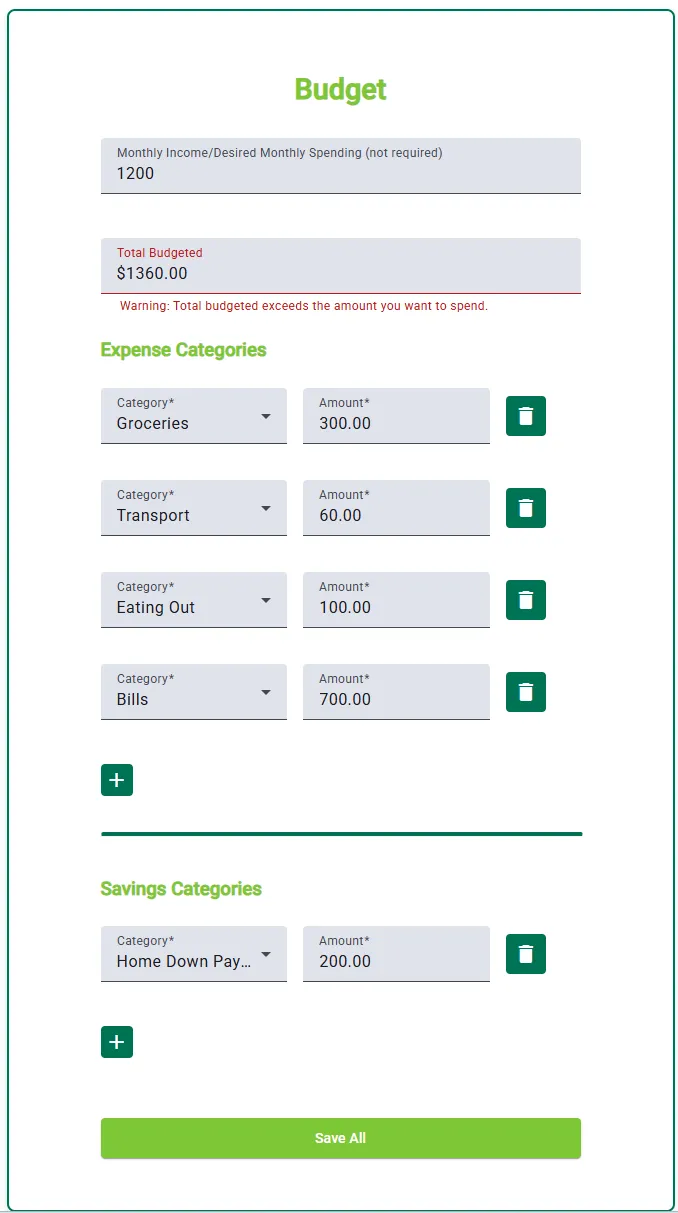
\includegraphics[width=0.3\linewidth]{images/UI-Screenshots/budget-form.png}
    \caption{The implemented budget form. Note the inputted desired spending amount and how this has led to a warning when the user's budget exceeds this amount.}
    \label{fig:budget-form}
\end{figure}

Displaying the user’s budget progress also required careful consideration. From the existing app comparison, it was clear that users appreciate visual representations of spending progress. To cater to this, watering cans were used to visually represent spending across each category. Each watering can fills in proportion to the amount spent and overflows when the budget is exceeded (see Figure \ref{fig:budget-page}). These were implemented using SVG graphics, with the water level calculated dynamically based on the percentage of the budget spent. If the user has spent more than the budgeted amount, a conditional check within the component displays a blue ellipse below the watering can, representing a spill. Additionally, a red dotted line surrounds the SVG container to further highlight overspending and to fulfil the MVP requirement for a clear visual indication in categories where the user has exceeded their budget.

\begin{figure}[htb]
    \centering
    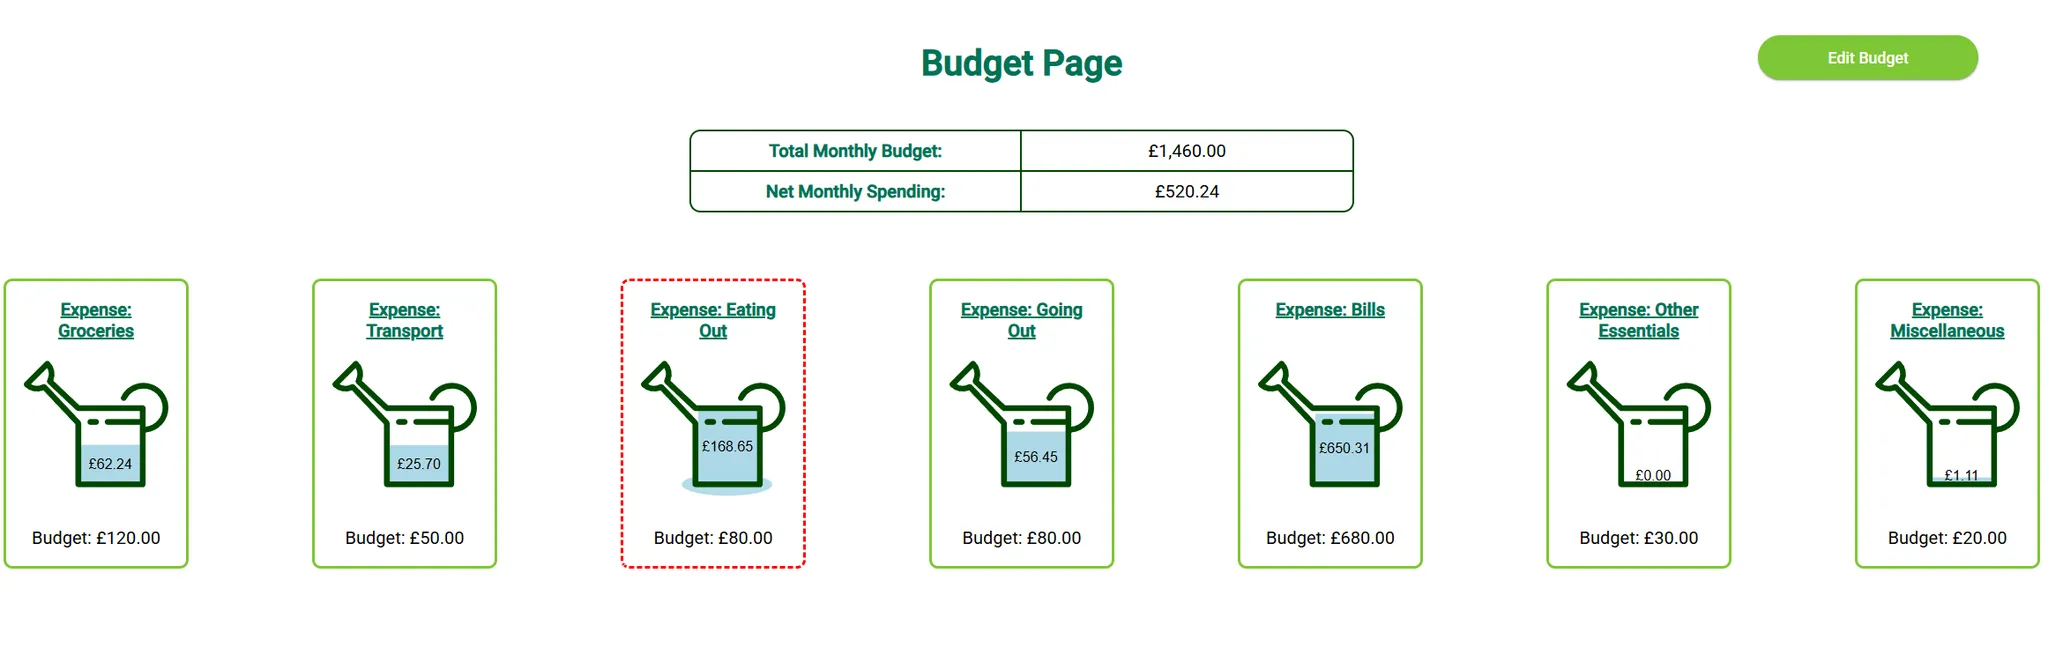
\includegraphics[width=0.75\linewidth]{images/UI-Screenshots/budget-page.png}
    \caption{The implemented budget page. Make note that each category in the users budget has their own watering cans and that categories that have been overspent in are illustrated clearly.}
    \label{fig:budget-page}
\end{figure}

The user can also view a table overview of their budget on the home page, providing an alternative, more data-driven view (see Figure \ref{fig:budget-table}). This table contains additional details such as how much the user has left to spend in each category, as well as a totals row summarising the amount spent overall and how much money remains for the current month.

\begin{figure}[htb]
    \centering
    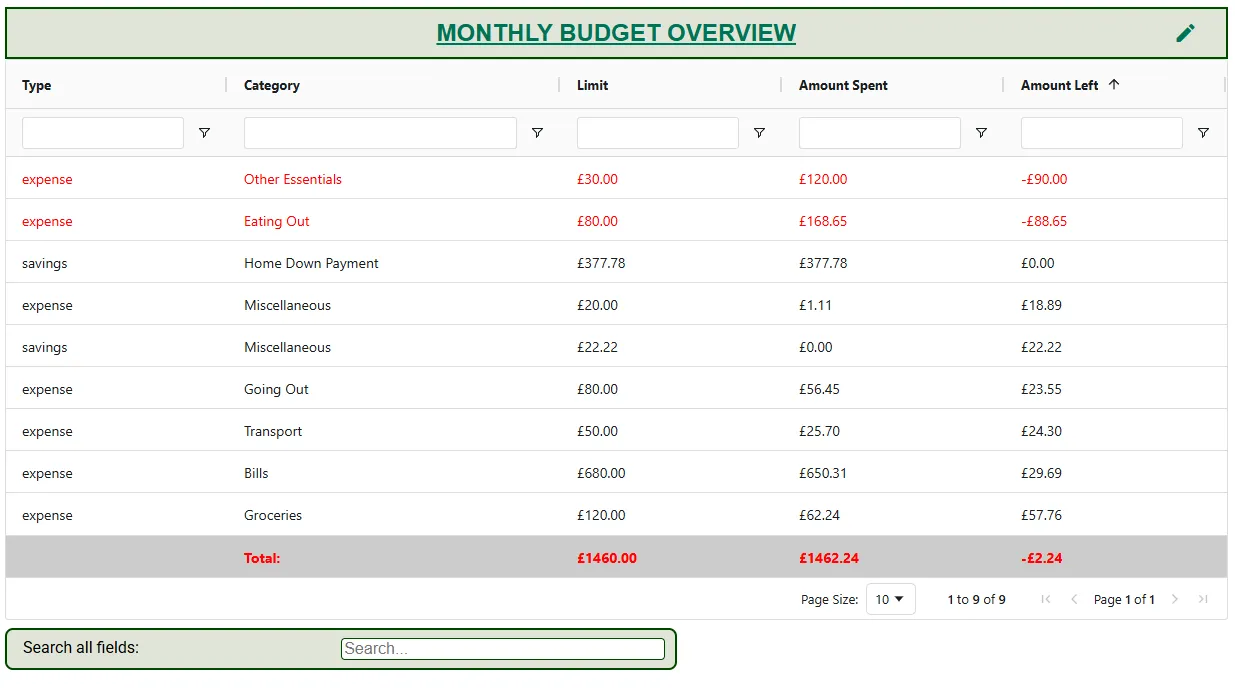
\includegraphics[width=0.75\linewidth]{images/UI-Screenshots/budget-table.png}
    \caption{The budget display from the home page. This is laid out like a data grid instead of the visual representation using the watering cans. Note that because the user has overspent on their entire budget, the totals row has turned red.}
    \label{fig:budget-table}
\end{figure}

In this display, any rows representing categories that have been overspent in are coloured red and appear at the top of the grid, prioritising visibility of categories requiring attention. Additionally, if the user has exceeded their overall budget, the totals row also turns red, offering a clear and immediate indication that spending limits have been surpassed.


\subsection{Setting \& Managing Savings Goals}
When designing the functionality for setting and monitoring savings goals, it was decided that contributions towards these goals would be based on a ranking system. Rather than assigning specific amounts to each goal manually, the total available savings are treated as a single pool of money that is distributed across the goals based on the user’s prioritisation. To facilitate this ranking mechanism, a drag-and-drop feature was implemented using an \citet{angular_material} component, allowing users to easily reorder their goals. When the order is changed, the distribution logic recalculates and the amount saved towards each goal updates instantly.

Each goal visualises the amount saved using a progress bar (see Figure \ref{fig:savings-area}), providing users with a quick visual reference of their progress. Goals can be edited or deleted after creation, with delete actions triggering a confirmation modal implemented using Angular Material’s dialog components.

\begin{figure}[htb]
    \centering
    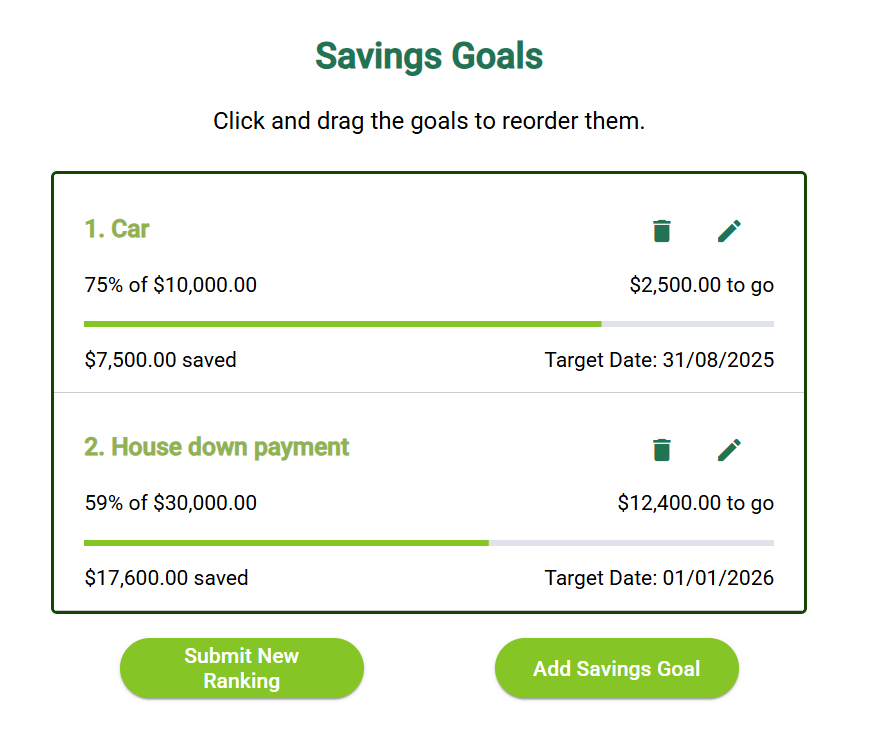
\includegraphics[width=0.35\linewidth]{images/UI-Screenshots/savings-goals-area.png}
    \caption{The savings goal area on the Savings page. Each goal can be dragged to change its ranking and the progress bar indicates how far the user is in completing their goal.}
    \label{fig:savings-area}
\end{figure}

A simplified overview of savings progress is also shown on the home page. This includes a progress bar representing how close the user is to reaching their combined savings targets.

\subsection{Logging Transactions}
Users can log transactions with detailed information along with if the transaction is repeated (see Figure \ref{fig:transaction-form}). These transactions are displayed using the \citet{ag_grid} library and are separated into two dynamically rendered tables: upcoming transactions and past transactions (see Figure \ref{fig:transaction-page}). This helps users easily distinguish between historical and future activity.

\begin{figure}[htb] 
    \centering
    \begin{subfigure}[b]{0.3\textwidth}
        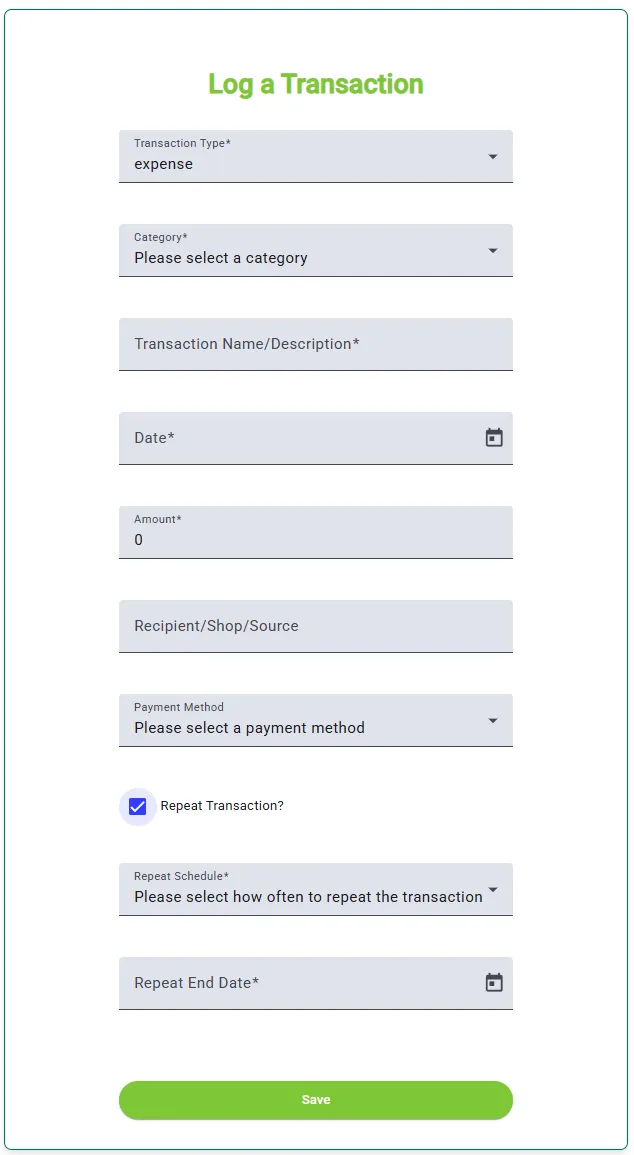
\includegraphics[width=\textwidth]{images/UI-Screenshots/transaction-form.png}
        \caption{The transaction form with each of the possible inputs displayed.}
        \label{fig:transaction-form}
    \end{subfigure}
    \hspace{1em}
    \begin{subfigure}[b]{0.31\textwidth}
        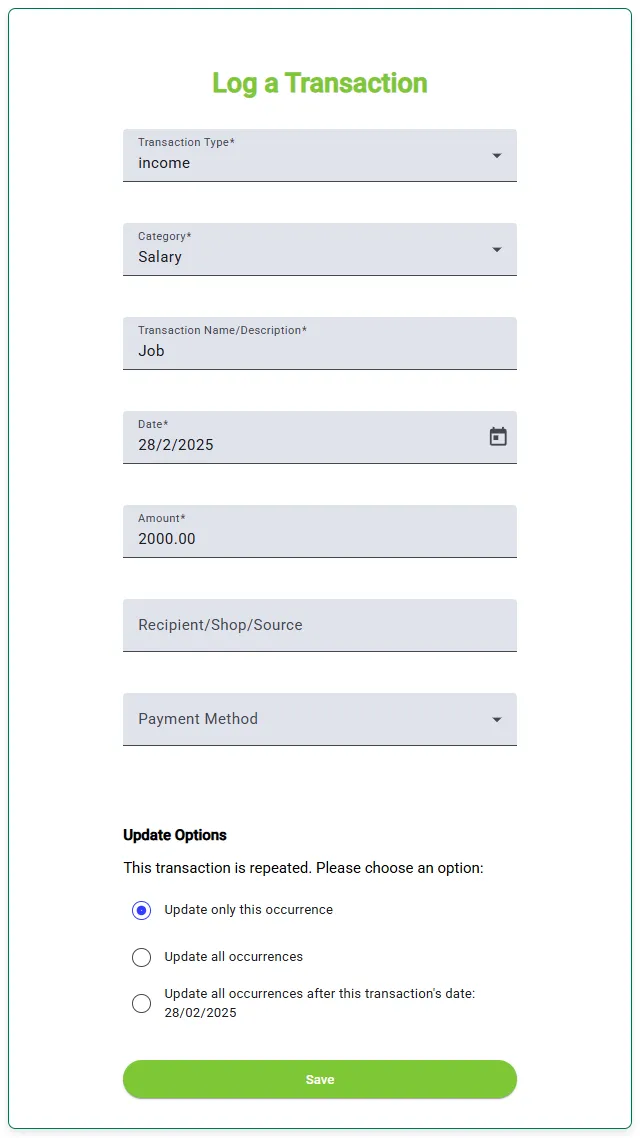
\includegraphics[width=\textwidth]{images/UI-Screenshots/transaction-form-edit.png}
        \caption{The display shown when editing a transaction that is repeated.}
        \label{fig:transaction-form-edit}
    \end{subfigure}   
    \caption{How the form is displayed for logging either a \subref{fig:transaction-form} new transaction or \subref{fig:transaction-form-edit} editing an existing, repeated transaction. Note in \subref{fig:transaction-form-edit} the update options at the bottom of the page that allow the user to customise how many transactions the changes are applied to.
    }\label{fig:screenshots}
\end{figure}

\begin{figure}[htb]
    \centering
    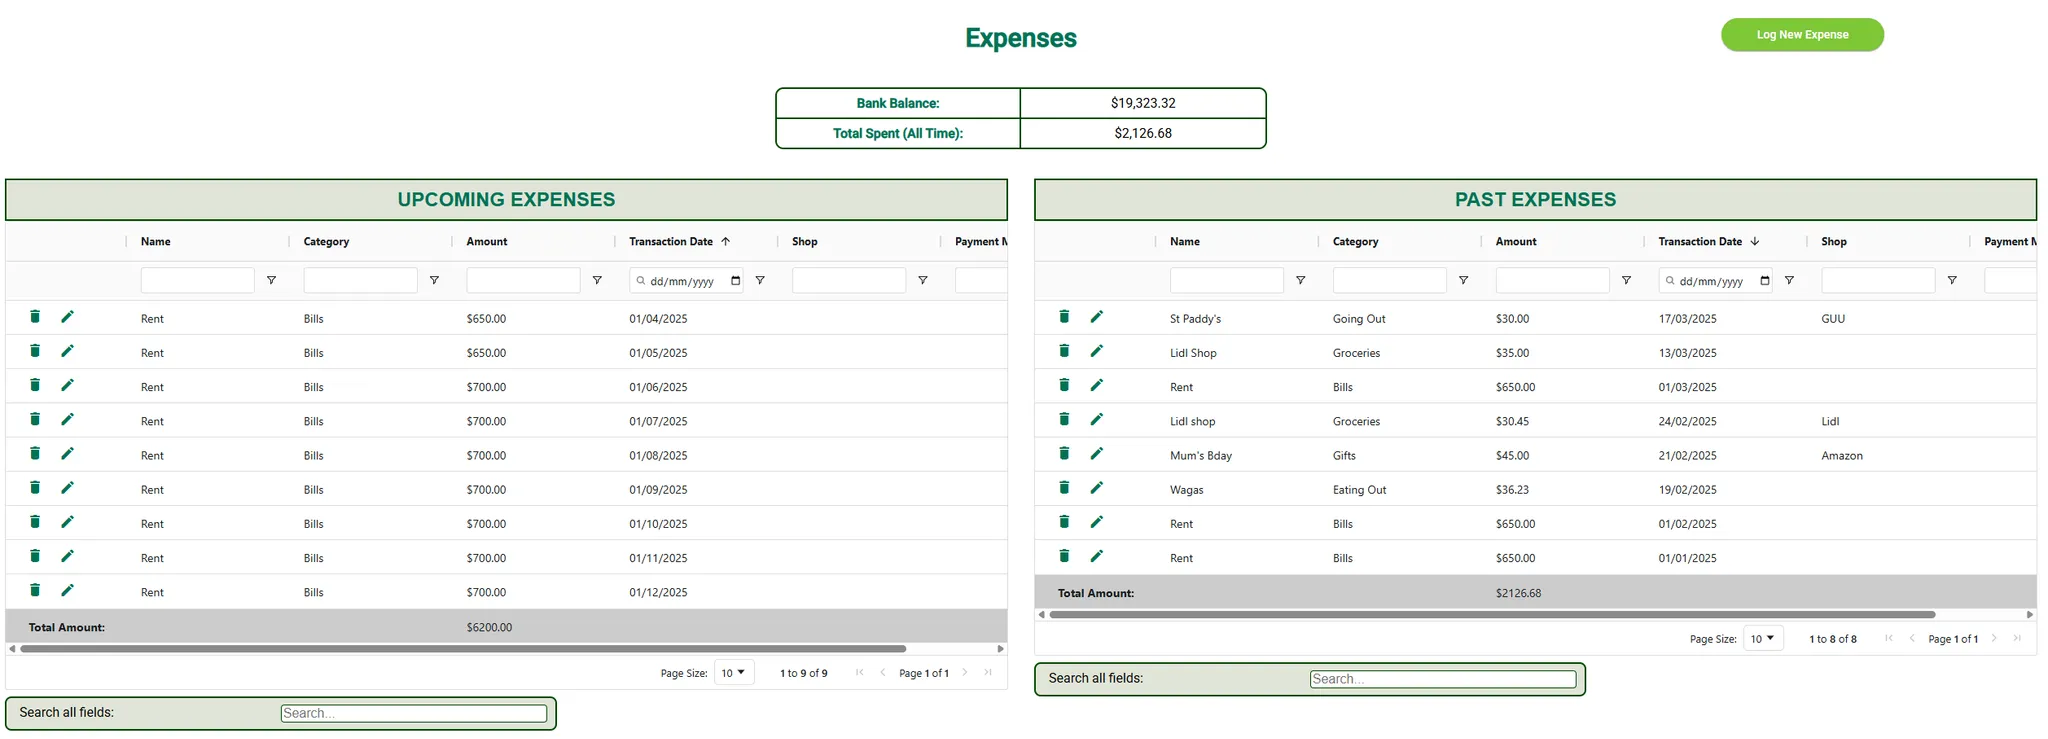
\includegraphics[width=\linewidth]{images/UI-Screenshots/transaction-page.png}
    \caption{The implemented expenses page. The savings and income pages look very similar. Note that transactions are split between two time periods and the custom search bar at the bottom of each table.}
    \label{fig:transaction-page}
\end{figure}

Handling repeated transactions required server-side logic to expand the initial input into multiple database entries. The user selects a repeat interval and an end date, and the server calculates each individual payment occurrence by mapping time intervals between the start and end date. Each occurrence is then expanded into a full transaction object with the original metadata and is inserted into the database in a single batch query. A unique repeat\_group\_id is generated and assigned to all instances, enabling batch operations (e.g. mass deletion or edits) later.

Both tables are sorted by transaction date, with custom sorting logic ensuring that transactions nearest to today’s date appear first. Since Angular defaults to the American date format of MM-DD-YYYY, a custom Moment.js data adapter was used to enforce the British format (DD-MM-YYYY).

AG Grid’s built-in column filtering and sorting capabilities were extended through custom comparator functions to ensure accurate date ordering and search functionality. Date filters were custom developed using a comparator-based IDateFilterParams implementation to allow date cells to be compared between rows. Although AG Grid supports individual column filtering, a custom search bar was implemented to enable full-table filtering via the quickFilterText property in the grid’s API.

For editing and deleting transactions, a reusable TableActionComponent was created to display edit and delete symbols and to support row-level modification of data. When modifying or deleting an entry that is part of a repeated transaction group, users are presented with multiple options: apply the action to a single transaction, to all occurrences of the transaction, or only to future occurrences (see Figures \ref{fig:transaction-form-edit}). These options are displayed in the log transaction form if the user attempted to edit the transaction and in a Material dialog popup component if attempting to delete one.

\subsection{Reports \& Charts}
Reporting and financial visualisation were highlighted as a priority during the user survey, so it was essential that the charts implemented were not only accurate but also easy to interpret. Three types of charts were developed (see Figure \ref{fig:charts}): a pie chart showing a breakdown of categories; a line graph tracking changes in the user's net balance over time; and a bar chart displaying which time periods involved the highest spending. Each chart supports customisation by reporting period (weekly, monthly or yearly) while the pie chart can also be filtered to show income, expenses, or savings categories.

\begin{figure}[htb] 
    \centering
    \begin{subfigure}[b]{0.3\textwidth}
        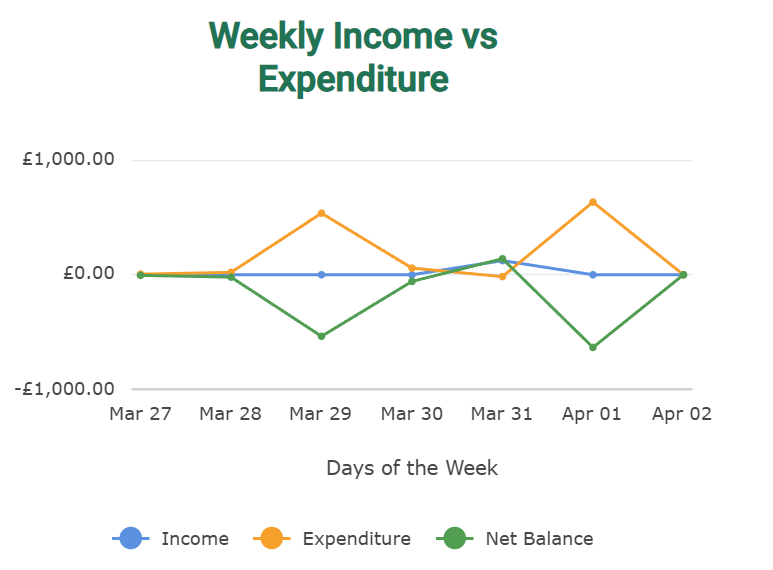
\includegraphics[width=\textwidth]{images/UI-Screenshots/line-graph.png}
        \caption{A graph depicting the user's net balance over the last week.}
        \label{fig:line-graph}
    \end{subfigure}
    \hspace{0.5em}
    \begin{subfigure}[b]{0.3\textwidth}
        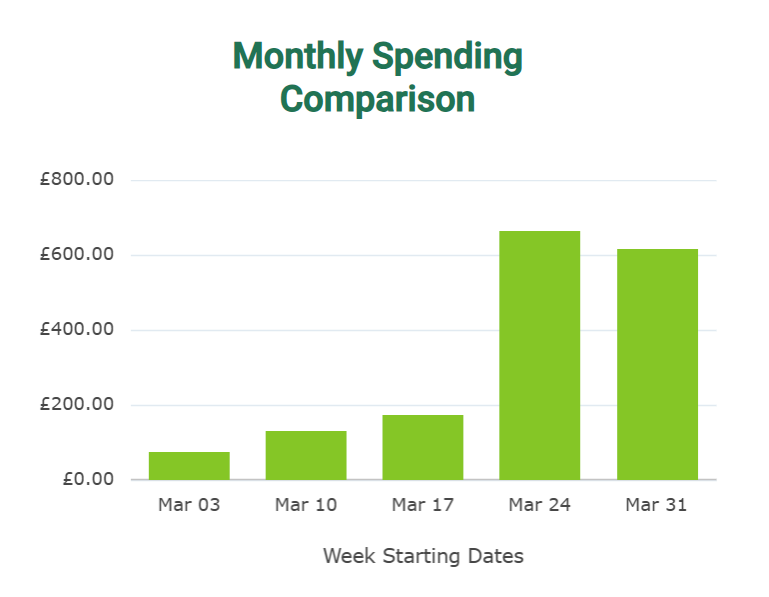
\includegraphics[width=\textwidth]{images/UI-Screenshots/bar-graph.png}
        \caption{A bar chart illustrating how much has been spent each week for the last month.}
        \label{fig:bar-graph}
    \end{subfigure}
    \hspace{0.5em}
    \begin{subfigure}[b]{0.3\textwidth}
        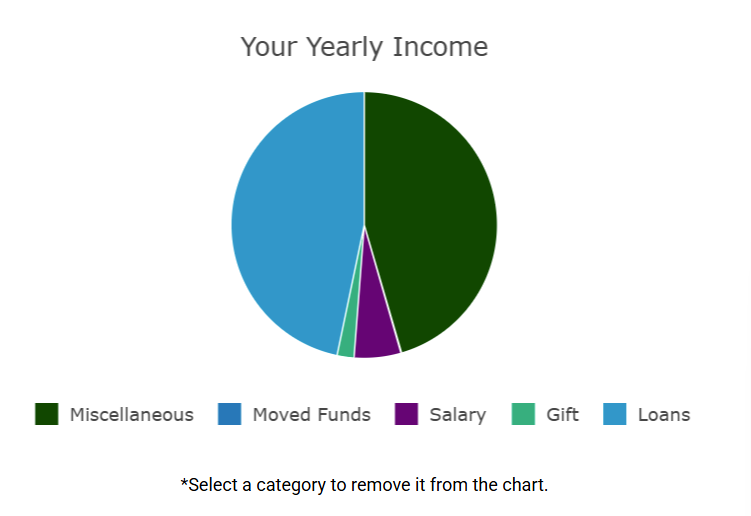
\includegraphics[width=\textwidth]{images/UI-Screenshots/pie-chart.png}
        \caption{A pie chart that shows the breakdown of the users income in the last year by category.}
        \label{fig:pie-chart}
    \end{subfigure} 
    \caption{The reports/charts found on the reports page. Each show the chart in a different reporting period. The pie chart can also show expenses and savings breakdowns.}\label{fig:charts}
\end{figure}

To handle situations where there might be no transactions in certain periods, the system uses Common Table Expressions (CTEs) with generate\_series(). This creates a full list of dates (or weeks/months), even when no data exists for them. By doing this, charts always show complete time ranges without gaps, and zero values are filled in using COALESCE() to keep the data consistent.

Each query also calculates income, expenses, and net totals (income minus expenses) directly in the database. This reduces the amount of processing needed on the frontend and makes the system faster and easier to work with.

\section{User Interface}
\subsection{Phone vs Desktop Views}
To ensure the maximal display on both phones and desktops, alternative styling was developed for each page to accommodate different screen sizes. This was achieved through the use of responsive components such as flexboxes, CSS grids and flexible sizing units such as fr, rem and percentages. These methods, combined with media queries, which trigger different CSS styling when the screen size drops below a set limit, allowed components to adjust depending on the device being used. CSS grids were particularly useful, as they allowed for structured positioning and provided a more reliable layout than some of the other methods such as flexboxes.

Challenges arose when using external libraries like AG Grid to display data. Although AG Grid is designed to efficiently handle large datasets, its styling was difficult to override, resulting in poor display on smaller screens. Similar issues were encountered with other libraries, such as Angular Material’s drag-and-drop elements, which had fixed minimum sizes that exceeded mobile screen widths and were difficult or impossible to customise. 

The data grids themselves also became harder to use on mobile, as only a few columns were visible at once. To improve readability, the past and upcoming transaction tables were stacked vertically on smaller screens. While rotating the phone to landscape mode alleviated some issues, relying on this is not ideal. Overall, the use of external libraries limited layout flexibility and mobile responsiveness.

Angular Material provided a consistent, modern UI across the app with reusable components like buttons, forms, popups, and drag-and-drop features (see Figure \ref{fig:savings-area}). Combined with Angular’s component-based structure, this enabled reusable modules, ensuring visual consistency and reducing redundancy through dynamic, flexible components.

\subsection{Scalable Data Management \& Performance Optimisation}
Handling large volumes of data was anticipated from the beginning of the project, particularly for users viewing their full transaction history.

AG Grid was chosen for its high-performance design, especially in handling large datasets. Beyond performance, AG Grid also helped reduce development time, as it came with many of the features required for displaying and interacting with transaction data, such as searching, sorting, and filtering, already built in. Although, AG Grid provided strong performance benefits and detailed documentation, the tables were hard to customise. Altering default styling or certain behaviours, such as filter interactions, was often challenging and lacked flexibility.

When it came to the data visualisation portion of the application, the \citet{ag_charts} library was used. This library is designed to work efficiently with complex datasets and supports interactive, high-performance charts. However, similar to AG Grid, AG Charts also limited the level of customisation available, particularly in terms of styling. As a result, certain design requirements involved complex workarounds, making the customisation process more difficult than expected.


\section{SQL Queries \& Server-Database Interaction}
An Express.js server was used to handle backend logic and database interactions, structured with a clear separation of concerns. All database logic was organised within an api folder, with a dedicated database-queries directory where each file, contained the SQL logic for a specific entity.

To keep the codebase modular and maintainable, the routing layer simply handled HTTP requests and passed data to these query files. This followed the Single Responsibility Principle, where each function focused on one task, such as inserting a transaction or updating a budget, making the code easier to test and debug.

Performance was prioritised through optimised SQL queries, indexing key columns like user\_id and transaction\_date, and using aggregation functions such as SUM, COUNT, and JOIN to offload calculations to the database. Queries were written to retrieve only the required data.

The backend followed RESTful API conventions, and a central query service was created on the frontend to manage API calls, keeping components cleaner and the codebase more maintainable.

Connection pooling was implemented using PostgreSQL’s Pool to efficiently manage and reuse database connections. This, along with careful handling of concurrent requests, ensured good scalability and responsiveness under load.

\section{Security}
\label{sec:security}
Given that the application handles user financial information, security was at the forefront of the design and development process. This section details the measures taken to protect the system against common attacks and security breaches.

\subsection{Protection Against SQL Injection}
SQL injection is a common attack in which a malicious actor manipulates SQL queries by injecting malicious code into form inputs or URL parameters. If not handled properly, this can allow attackers to access, modify, or delete database records, sometimes even bypassing user authentication altogether \citep{w3_schools_sql_injection}.  

To reduce this risk, all database communication in the system is handled using parameterised queries. These queries use placeholders (e.g. \$1, \$2) rather than embedding values from the user directly into the SQL query strings. Values are bound to these placeholders at execution time, preventing any injected SQL code from being interpreted as part of the query logic. 

Additionally, routes on the server are protected by an authentication middleware which verifies the user’s identity before the database query is even reached. This adds an additional layer of protection, as even valid SQL queries cannot be executed unless the user provides a valid access token.


\subsection{Authentication \& Session Management}
\label{sec:jwt}
User authentication is handled using JSON Web Tokens (JWTs), which are securely generated and signed when a user logs in. Upon successful login, the server creates a token using a secret key, embedding the user’s ID in the payload. This token is then returned to the client and used to authenticate future requests. This system was implemented with the help of a \citet{geeksforgeeks_jwt_authentication} tutorial.

Each protected route on the server checks the incoming request for a valid token using an authentication middleware. The token is extracted from the Authorization header, and is verified using the same secret key that was used at login (see Appendix \ref{app:auth-middleware} for the middleware code). If the token is missing or invalid, the server immediately rejects the request, returning an error response and then logs the user out.

These JWTs automatically expire after one hour. This helps to minimise the risk of long-term session hijacking, even in cases where the token is somehow illegitimately accessed. While storing the token in an HTTP-only cookie was attempted for added protection against client-side attacks, it was eventually stored in sessionStorage due to compatibility issues and to maintain simplicity in the Angular frontend. Although sessionStorage is accessible to JavaScript, it is automatically cleared when the browser tab is closed, making it a safer option than localStorage, which keeps data indefinitely.

\subsection{Password Security}
Password logic and security are handled entirely in the database. When a user creates an account or logs in, their password is hashed using pgcrypto’s crypt function and a unique salt, generated using the Blowfish algorithm. This process was developed with the help of a \citet{vultr_passwords_postgresql} tutorial on securely saving passwords using PostgreSQL. Only the resulting hash is stored in the database, and plain-text passwords are never saved.

Earlier versions of the system temporarily stored the hashed password in localStorage to simplify login handling. However, this approach was deemed insecure, as client-side storage of even hashed passwords increases exposure to cross-site scripting (XSS) attacks \citep{owasp_html5}. This practice was removed in favour of token-based session management. At no point in the current implementation is the user’s password or hash ever stored on the client or even transmitted from the database after the initial login.

\subsection{Cross-Origin Resource Sharing (CORS) }
\label{sec:cors}
CORS configuration plays an important role in determining which frontend domains are allowed to access the server \citep{aws_cors}.

The server checks the origin of each request against a list of trusted domains. Only requests from the deployed frontend or from localhost (when in development or test mode) are allowed. If a request comes from an unrecognised domain, it is immediately rejected with a 401 Unauthorised response. This ensures that external scripts or unauthorised web applications cannot access the server APIs even if they somehow acquire a valid token.

This CORS configuration is handled in a dedicated middleware file, which sets the appropriate response headers and performs origin checks before any further processing takes place. In addition to this, all production traffic is served over HTTPS, ensuring that sensitive data, including JWTs, is encrypted during transit.


\subsection{Managing Environment Variables}
Sensitive credentials such as database passwords, JWT secrets, and environment-specific configuration values are never hardcoded into the application source code. Instead, they are stored in environment variables, accessed through process.env.

In development, these values are defined in a local .env file, which is excluded from version control via .gitignore to prevent accidental disclosure. In production, environment variables are managed securely through the Vercel deployment dashboard. This ensures that critical secrets remain confidential and are not exposed on the client-side or version history.



\section{Deployment}
The initial deployment plan involved GitHub Pages, but it was quickly discovered that it only supports static web applications \citep{github_about_pages}. As the project included a Node.js server, this option was not viable.

Alternative hosting solutions were explored for the front-end, backend, and database. The first platform tested was \citet{vercel_docs}. Although the front-end rendered correctly, Vercel treated the project as a static site, breaking Angular’s routing. After several troubleshooting attempts, a modular deployment strategy was adopted.

The project was reinitialised without server-side rendering to simplify deployment. \citet{firebase} was then chosen to host the front-end, offering an easy setup for static content. However, it was not suitable for hosting the full-stack architecture.

The final deployment approach used Firebase for the Angular front-end, Vercel for the Node.js server, and \citet{supabase} for the PostgreSQL database. This introduced the need for cross-service HTTP communication and raised CORS issues due to separate domains. These were resolved through configuration changes, as discussed in Section \ref{sec:cors}.

Although deploying across multiple services added complexity, it allowed the use of free hosting platforms, aligning with the project's accessibility goals. It also offered flexibility and scalability for potential future development.


%==================================================================================================================================
\chapter{Evaluation} 

\section{Testing}
Unit tests were conducted to verify the system’s functionality at the component level, ensuring that each part of the application worked as expected in isolation. These tests are crucial for identifying issues early and maintaining stability throughout development, especially when implementing larger changes that could affect existing features.

Angular testing utilises the Jasmine and Karma frameworks. Jasmine provides a behaviour-driven development (BDD) framework for writing and structuring tests, while Karma acts as a test runner to execute them in real browsers.

All components underwent unit testing, achieving over 90\% coverage across the frontend, exceeding the industry standard of 80\%. A few components fell short of this threshold due to challenges with mocking external libraries, particularly Angular Material. Code coverage metrics are detailed in Appendix \ref{app:code-coverage-frontend}.

Frontend services, responsible for tasks like authentication, data querying, and component communication, were also thoroughly tested to ensure reliable system performance and minimise integration issues.

The backend server was tested using the Jest testing framework. Each file was rigorously tested, including those managing CORS access, middleware authentication, error handling, query pooling, database routes, and database queries. Integration tests were implemented to ensure smooth communication between the frontend, middleware, and database. These tests achieved over 90\% coverage, and the metrics are detailed in Appendix \ref{app:code-coverage-server}.

Automated testing was integrated into the CI/CD pipeline using GitHub Actions. This setup ensures that unit and integration tests are automatically executed whenever code is committed or a merge request is made, maintaining code quality and stability. By automating these tests, any issues introduced by new changes can be promptly identified, reducing the risk of regressions.

Beyond these formal testing strategies, usability testing was conducted through manual interaction with the application from an end-user perspective. This helped verify that common tasks, such as creating budgets and logging expenses, were intuitive and functioned correctly in real-world scenarios. User testing was also performed as part of the system evaluation and is discussed further in the next section.

Additionally, the user evaluation was used to test the database storage capabilities, as it was unclear how much data the system could handle. By recruiting participants for the study, it was possible to observe database performance under load. Even with 20 participants, each inputting close to 100 records, the database never approached its capacity and continued to operate effectively without noticeable performance degradation.

\section{Evaluation \& User Testing}
\subsection{Aims}
This evaluation assessed how well the application met the MVP requirements. Since these were based on end-user feedback from a user study and app reviews of existing budgeting applications, meeting them indicates alignment with user needs.

It also served as user testing, enabling direct observation of interactions with the system. In addition to assessing functionality, the study evaluated usability and overall experience. Through structured tasks and participant feedback, it identified strengths, usability issues, and areas for improvement.

\subsection{Evaluation Design}
A task-based evaluation was conducted to assess ease of use, feature effectiveness, and overall user perception. 

The evaluation had two phases: a supervised phase, where participants’ actions, challenges, and preferences were observed, followed by an unsupervised phase, where refined instructions were tested via a Microsoft Form. Participants completed a streamlined version of the same tasks independently, without real-time guidance during the unsupervised phase.

Participants provided demographic data on age, tech comfort, and budgeting habits before completing eight core tasks covering registration, budget creation, savings management, transaction logging, and financial reporting. Post-task questions gathered insights on usability, pain points, and overall experience. The full task list and questions are in Appendix \ref{app:ethics-questionnaires} and links to the complete form results can be found in Appendix \ref{app:result-links}.

The evaluation followed university ethical guidelines. Participants gave informed consent, could withdraw at any time, and no personally identifiable data was stored. The signed ethics checklist is in Appendix \ref{app:ethics-checklist}.


\subsection{Results}

The evaluation included 20 participants, 11 supervised and nine unsupervised, with most aged 18–25. Across all participants, banking apps were the most common method for managing finances, while only two participants used budgeting apps, specifically Emma, Lumio, and Snoop. Most people also reported that they review their budget weekly. Charts can be found in Appendix \ref{app:evaluation-charts}.

In the remote evaluation, five of nine participants used a computer, while three used their phones. Of these, two accessed the website, and only one downloaded the app. \\

\textbf{Task 1 - Registration \& Login}

All participants successfully created an account and logged in. A bug was discovered when a participant selected Czech Koruna as their currency, causing NaN errors in calculations due to the system assuming currency symbols were a single character. This was promptly fixed before the next evaluation.  

Users also highlighted a navigation issue, with seven of the 11 supervised participants expecting the Transactions heading in the navigation bar to be a link rather than a dropdown. \\

\textbf{Task 2 - Creating a Monthly Budget}

All participants successfully created budgets with the required amount by adding, editing, and deleting categories. 85\% found the process intuitive, with many highlighting the real-time budget total as particularly helpful. Positive feedback included 65\% finding it easy to use, 30\% appreciating the wide range of categories, and 25\% praising the clean UI and colour palette.  

However, some issues were raised. The field for setting a desired budget total was unclear to users, and warnings for exceeding this amount lacked visibility. Additionally, premature form submission when pressing Enter and dropdown text being cut off on mobile were noted. \\  

\textbf{Tasks 3 \& 7 - Setting \& Managing Savings Goals} 

Participants found the UI intuitive, with the drag-and-drop feature for reprioritising goals being well received. However, several participants expected automatic saving of the reorder instead of manual confirmation. While 90\% understood how goal order affected distribution, only 35\% fully grasped where the redistributed money originated. Several participants requested the ability to allocate specific transactions to savings goals rather than relying solely on automatic fund distribution.  

Some struggled to find the Savings page under the Transactions drop-down and suggested a separate menu item. Additionally, participants had difficulty finding the Add Savings Goal button as it was often positioned lower down and required scrolling to be seen.  \\ 

\textbf{Tasks 4 \& 5 - Adding Income \& Expenses}

Most participants found adding both singular and recurring transactions easy. However, some attempted to enter expenses directly into the grid rather than using the Add Transaction button.  

Filtering by date was a major usability issue, with all supervised participants struggling to locate or understand the filter button. Recurring transactions also presented challenges, with users finding the delete workflow unintuitive and requesting more flexibility in editing repeat logic after transaction creation. \\

\textbf{Task 6 - PWA Mobile App}

Among supervised participants, 80\% attempted to use the PWA mobile app, but 50\% switched back to desktop due to layout issues, difficulties with tables, and a preference for larger screens.  \\

\textbf{Task 8 - Viewing the Budget \& Home Page}

Preferences were mixed between the Budget and Home pages for viewing financial summaries. The Budget page was preferred for clarity, while the Home page provided more information but could feel overwhelming, particularly on mobile.  

No participants found the Add Savings Goal button on the Home page, as the flag icon used for this action was unintuitive.  \\

\textbf{Task 9 - Viewing Reports \& Charts}

Most users successfully interacted with the reporting features, though some struggled with removing categories due to unclear selection functionality. Suggestions included a bar chart alternative for the pie chart and clearer differentiation of net income/expenditure trends.  

\subsection{Discussion}

The evaluation demonstrated that the budgeting system is generally intuitive and user-friendly, with a clean design and strong visual appeal. However, several usability issues were identified, particularly around navigation, mobile usability, and transaction management.  \\

\textbf{Navigation \& Mobile Usability}

Navigation was largely well received, but some users found certain elements unintuitive, particularly the placement of savings under Transactions and the flag icon for adding savings goals. The mobile version was useful for quick access but had layout issues, especially with tables and dropdowns, which impacted usability. Enhancements such as clearer icons, better spacing, and improved table responsiveness would improve the mobile experience.  \\ 

\textbf{Budgeting \& Savings Features}

While creating a budget was straightforward for most, the lack of visibility for overspending warnings and the unclear nature of the budget total field were recurring concerns. Addressing these by improving warning placement could enhance user understanding.  

Savings goals were well received overall, but participants desired greater manual control over savings allocation. The ability to assign transactions directly to specific goals could increase user flexibility and engagement.  \\

\textbf{Transaction Management \& Filtering}

Filtering transactions was one of the most significant usability challenges, with multiple participants struggling to locate or use the filtering options. A more prominent filter button, clearer explanations, and a simplified rule-setting interface could address this issue.  

Recurring transactions also required improvement. Many users instinctively attempted to delete recurring transactions by setting their value to zero rather than using the Delete button. Additionally, users wanted more flexibility in scheduling transactions (e.g. repeating on “the last Thursday of the month”). Enhancing the edit functionality and introducing a clearer deletion workflow would improve user experience.  \\

\textbf{Reporting \& Data Visualisation}

Participants appreciated the reporting features, but interaction with charts was sometimes unclear. Providing alternative chart types and improving interactivity, such as hover tooltips and checkboxes for filtering categories, would improve the experience. \\

\textbf{Feature Requests}

Many participants who did not already budget found the app helpful and indicated they would use it. However, spreadsheet users preferred their existing methods due to familiarity and flexibility. Bank integration was highlighted as a key factor that would encourage adoption, along with customisable categories and CSV transaction imports.  

Despite some usability challenges, overall reception was positive, with 55\% of participants stating they would use the application over their current method. Participants appreciated the app’s visuals, intuitive design, and user-friendly approach. One participant mentioned that the app made them want to budget and asked when the final product would be available. Several others expressed interest in continued use. 

\subsection{MVP Requirements Evaluation}
\begin{table}[H]
    \centering
    \begin{tabular}{|p{5cm}|p{2.5cm}|c|p{5cm}|}
        \hline
        \textbf{Requirement} & \textbf{Relevant Tasks} & \textbf{Met?} & \textbf{Comments} \\
        \hline
        Secure login and data protection & 1 & \ding{51} & Login worked as expected with several security measures in place. \\
        \hline
        Set default currency on account setup & 1 & \ding{51} & Initially buggy with non-standard currency symbols but resolved. \\
        \hline
        Log spending and income with appropriate detail & 4, 5, 7 & \ding{51} & Process was intuitive, but some users expected direct grid entry for expenses. \\
        \hline
        Edit/delete transactions (including repeated transactions) & 4, 5, 7 & \ding{51} & Users could edit/delete, but recurring transaction deletion was unclear and led to confusion. \\
        \hline
        View reports/charts on finances & 9 & \ding{51} & Users found graphs helpful but suggested more interactivity and alternative chart types. \\
        \hline
        Set and track budgets & 2, 8 & \ding{51} & Budgeting was well-received, with both the grid and watering can formats praised for different reasons. \\
        \hline
        Set and track savings goals & 3, 7 & \ding{51} & Many appreciated the process, however, goal handling did receive some criticism, including how savings were assigned to each goal. \\
        \hline
        Persistent storage of user data & \textasteriskcentered{} & \ding{51} & User data remained after leaving, meeting expectation. \\
        \hline
        Indicate overspending in a clear way (category level) & 2, 8 & \ding{51} & Both the watering can approach and the table rows turning red to indicate overspending, were noted as positives of the system. \\
        \hline
        Indicate overall budget overspending clearly & 2, 8 & \ding{55} & No clear notification system for budget overspending; users were unsure of where this information would be displayed. \\
        \hline
        Check funds for upcoming expenses & 4, 5, 8 & \ding{51} & Users could check upcoming expenses, but filtering by date was confusing. \\
        \hline
        Mobile-friendly design with PWA capability & 6 & \ding{55} & Mobile layout had usability issues, particularly with tables and navigation. \\
        \hline
    \end{tabular}
\end{table}


\subsection{Implications for App Improvements}  
The evaluation demonstrated that the budgeting system is intuitive and user-friendly, with strong visual appeal and useful features. However, improvements are needed in:
\begin{itemize} \item Enhancing mobile usability, especially for tables and navigation.
\item Improving feature visibility, such as the savings goals icon on the Home page and overspending warnings.
\item Refining transaction workflows, including filtering and recurring transaction edits
\item Providing more user control over savings allocation and enhancing reporting flexibility.
\end{itemize}

Despite these challenges, participants showed enthusiasm for the app. With
targeted refinements, it has strong potential for adoption and user satisfaction.

%==================================================================================================================================
\chapter{Conclusion}

\section{Summary}
Budgeting is an essential life skill that can significantly improve quality of life and mental well-being by giving individuals greater control over their money and spending. Technology is a powerful tool for financial management, leveraging data analysis and the ubiquity of mobile devices to enable detailed and informed tracking on the go.

Many applications already utilise these capabilities but often fall short in different ways. Some are overwhelmingly flexible (e.g. spreadsheets), while others require payment and abstract the budgeting process too far, resulting in rigid solutions. By comparing existing solutions, gathering feedback through personal usage, and analysing app store reviews, a concrete set of requirements for a new system was established. These requirements were further refined through an end-user survey, gathering insights into current budgeting practices and desired features.

The chosen architecture was a Progressive Web Application (PWA) comprising an Angular frontend, a Node.js server, and a PostgreSQL database. This approach enabled free web deployment while offering a mobile app experience, ensuring accessibility without financial barriers. The design prioritised a mobile-friendly, intuitive system with a clean UI that contained all necessary features without being overwhelming. Visualisation was a key aspect, with watering can icons designed as progress bars for each budget category.

Implementation followed sound software engineering practices, including version control with Git and GitHub, feature branching, a Kanban board for issue tracking, and continuous deployment to Firebase for the frontend, Vercel for the server, and Supabase for the database.

All planned features were implemented, with adjustments to savings goals and navigation to enhance usability. Due to the sensitive nature of financial data, security was prioritised through measures such as password hashing with salts, JSON Web Tokens for authentication, parameterised queries to guard against SQL injection, and CORS policies to prevent unauthorised server access.

Both monitored and unmonitored evaluations were conducted to assess the system’s performance, identify areas for improvement, and carry out user testing. This led to resolving issues like multi-character currency code handling. Evaluations indicated that the system effectively met the requirements, with many users expressing interest in continued use. Participants praised the clean UI, clear visualisation of savings goals and budget progress, and the availability of financial reports. However, some found certain features confusing, such as filtering transaction tables by date, and the mobile version had usability issues like unintended touch interactions and layout problems on smaller screens. While users generally liked the system, some remained hesitant due to being comfortable with existing methods and the lack of bank integration.

In conclusion, the project successfully achieved its goal of creating a personal budgeting application that supports spending, income, and savings goal tracking, along with reporting and budget management. However, further improvements are needed to fully meet the diverse needs of a broader user base and ensure usability on mobile devices.


\section{Future work}
% Discuss what you would do if you could take this further -- where would the interesting directions to go next be? (e.g. you got another year to work on it, or you started a company to work on this, or you pursued a PhD on this topic)
The following section discusses potential changes and enhancements that could be implemented in the app if there was more time in the project or if the project is developed further in the future.

\subsection{Enhancing Mobile Usability}

The current application does not work effectively on smaller touchscreen devices, which was a major requirement for the project. Improvements could include resizing elements to fit the screen, potentially involving switching libraries, or blocking column movement in tables to prevent accidental rearrangement and loss of columns.

Larger changes could also enhance the mobile experience. Since grids are difficult to view on smaller screens, the table view could be redesigned to display just the transaction name, date, and amount, with more details shown on click. This would present essential information at a glance while allowing users to view more as needed.

\subsection{Expanding Reporting \& Customisation Options}

Currently, users can only view reports for the current week, month, or year. It would be beneficial to allow viewing of past periods, such as previous months or years, enabling better financial analysis and decision-making.

Reports could also be made more customisable. Rather than just breaking down spending by category, users could choose to see breakdowns by shop/payee or payment method. Additionally, more reporting periods could be offered, such as fortnightly, payday-to-payday, or custom. Users could also select their preferred chart type (e.g. bar graph instead of pie chart).

Preferences like chart types, reporting periods, and transaction table ordering could be saved to the user’s account to provide a consistent experience when logging in.

\subsection{Custom Categories \& Multiple Bank Account Support}

Additional features from the "should have" and "could have" sections of the MoSCoW prioritisation could be added to increase flexibility. Allowing users to create custom categories would enable them to tailor budgeting and tracking to their specific needs.

Implementing multiple bank account support could also help users track spending across various accounts (e.g. savings, current, ISAs). Interest rates could be linked to these accounts, allowing the system to automatically calculate interest payments.

\subsection{Linking Savings to Specific Goals}

Currently, savings are treated as one collective pool that trickles down through goals based on prioritisation. It would be beneficial to let users allocate savings to specific goals, creating custom savings categories that give more control over where transactions are directed. Generic savings could still follow the trickle method for those who prefer it.

If combined with the ability to track multiple bank accounts, users could tie specific accounts to particular savings goals or allocate a percentage of an account balance to a goal.

\subsection{Optional Bank Integration}

Some evaluation participants expressed interest in Open Banking integration to avoid manual transaction logging. However, the initial decision to exclude this feature was due to time constraints and feedback indicating that manual entry increases accountability and trust. Additionally, many existing apps that require Open Banking are are unusable without this integration, which was a main complaint during the existing app comparison.

To meet the desire for bank integration without compromising flexibility, this feature could be made optional, allowing users to decide whether to connect their accounts. Enhanced security measures, such as two-factor authentication and robust data protection, would be necessary to handle the additional sensitive information.

\section{Reflection}
This project was a valuable learning experience in designing, implementing, and managing a full-stack application. Simultaneously developing frontend, server, and database capabilities required significant organisation and thorough checks to ensure that all components behaved as expected. The adoption of sound software engineering practices greatly supported this process. In particular, the Kanban board proved invaluable for tracking issues, keeping tasks on schedule, and maintaining clarity in the future workflow. Additionally, continuous deployment allowed new features to be tested in production environments, ensuring compatibility with production technologies and preventing unexpected breakages.

A substantial amount of time was dedicated to analysing requirements and designing the system, which proved beneficial once implementation began. However, some challenges could not be fully predicted or planned for, making it essential to remain flexible and make informed decisions throughout development. Despite the extensive planning, some key objectives lost focus during implementation, most notably, mobile usability. Since development primarily took place on a computer, much of the styling and features were optimised for desktop use, with insufficient testing on mobile devices. In hindsight, a more mobile-focused technology stack would have maintained emphasis on mobile usability, even at the cost of ease of deployment and accessibility.

Testing practices also emerged as a weakness during the project, as they were not consistently incorporated from the outset. Although continuous deployment was maintained, the absence of early testing meant that bugs occasionally reached production or were not identified promptly. Future projects would benefit from adopting a test-driven development approach by writing tests alongside the code and establishing an automated testing pipeline from the beginning. This would ensure that no code could be deployed to production without passing essential checks.

Overall, many of the project requirements were successfully met, and the evaluation received largely positive feedback from the 20 participants. Throughout the process, valuable technical skills were developed, including making database queries through HTTP calls, implementing secure page access with Angular routing, and applying security measures to protect sensitive data. Important soft skills were also cultivated, such as feature prioritisation as deadlines approached and maintaining consistent documentation of completed work.

Ultimately, the Evergreen Budgeting app achieved its primary goal of providing users with an effective tool for tracking and managing personal finances through a calming and aesthetic UI. The insights gained from this experience will significantly inform future development efforts.

%==================================================================================================================================
%
% 
%==================================================================================================================================
%  APPENDICES  

\begin{appendices}

\chapter{Detailed Existing App Comparison}
\label{app:app-comparison}
\section{GoodBudget}

GoodBudget is a manual-entry budgeting app based on the envelope budgeting strategy. It is available in both free and paid versions, though the free version limits the number of envelopes users can create and the number of bank accounts they can track. There is also a web-based version of the app, which appears to be more complex and feature-rich than the mobile version. However, since this analysis focuses on mobile applications, the web version was not examined in detail.

\vspace{0.5em}
\textbf{Key features:}
\begin{itemize}
    \item "Envelopes" to categorise and track spending
    \item Debt-payment tracker
    \item In-app reports/charts to monitor budgeting progress
    \item Manual transaction entry including details such as payee, transaction amount, envelope category, and transaction date
    \item Ability to sync across devices (paid version only)
    \item Notifications to encourage progress or warn when overspending occurs
\end{itemize}

\vspace{0.5em}
\textbf{Strengths/positive feedback (Google Play Store reviews):}
\begin{itemize}
    \item Simplistic UI that is easy to use
    \item Informative and encouraging notifications
    \item No requirement to link to a bank account
    \item Manually adding transactions increases user accountability for spending
    \item Data syncs across devices (available in the paid version)
\end{itemize}

\vspace{0.5em}
\textbf{Limitations/negative feedback (Google Play Store reviews):}
\begin{itemize}
    \item Minimal reports/charts available and lack of customisability of these reports available
    \item Confusing process for editing envelope capacities on a one-time basis
    \item Inconsistencies between the mobile and web app experiences
    \item Many features are locked behind a paywall
\end{itemize}

\vspace{0.5em}
\textbf{Observations/personal experience:}
\begin{itemize}
    \item The envelope system was simple and easy to grasp.
    \item Progress bars for each envelope category were visually effective in communicating spending at a glance.
    \item The app does not require linking to a bank account, which may feel more secure for some users, especially when initially trying out the platform.
    \item The free version was rather limited.
    \item The lack of customisability in reports limited financial insights.
    \item Transactions were added to the bank balance even when the scheduled transaction date had not yet passed.
    \item Repeat payment schedules were limited and did not offer an end date, resulting in indefinite repetition.
\end{itemize}



\begin{figure}[h]
    \centering
    \begin{subfigure}[t]{0.25\textwidth}
        \vspace{0pt}
        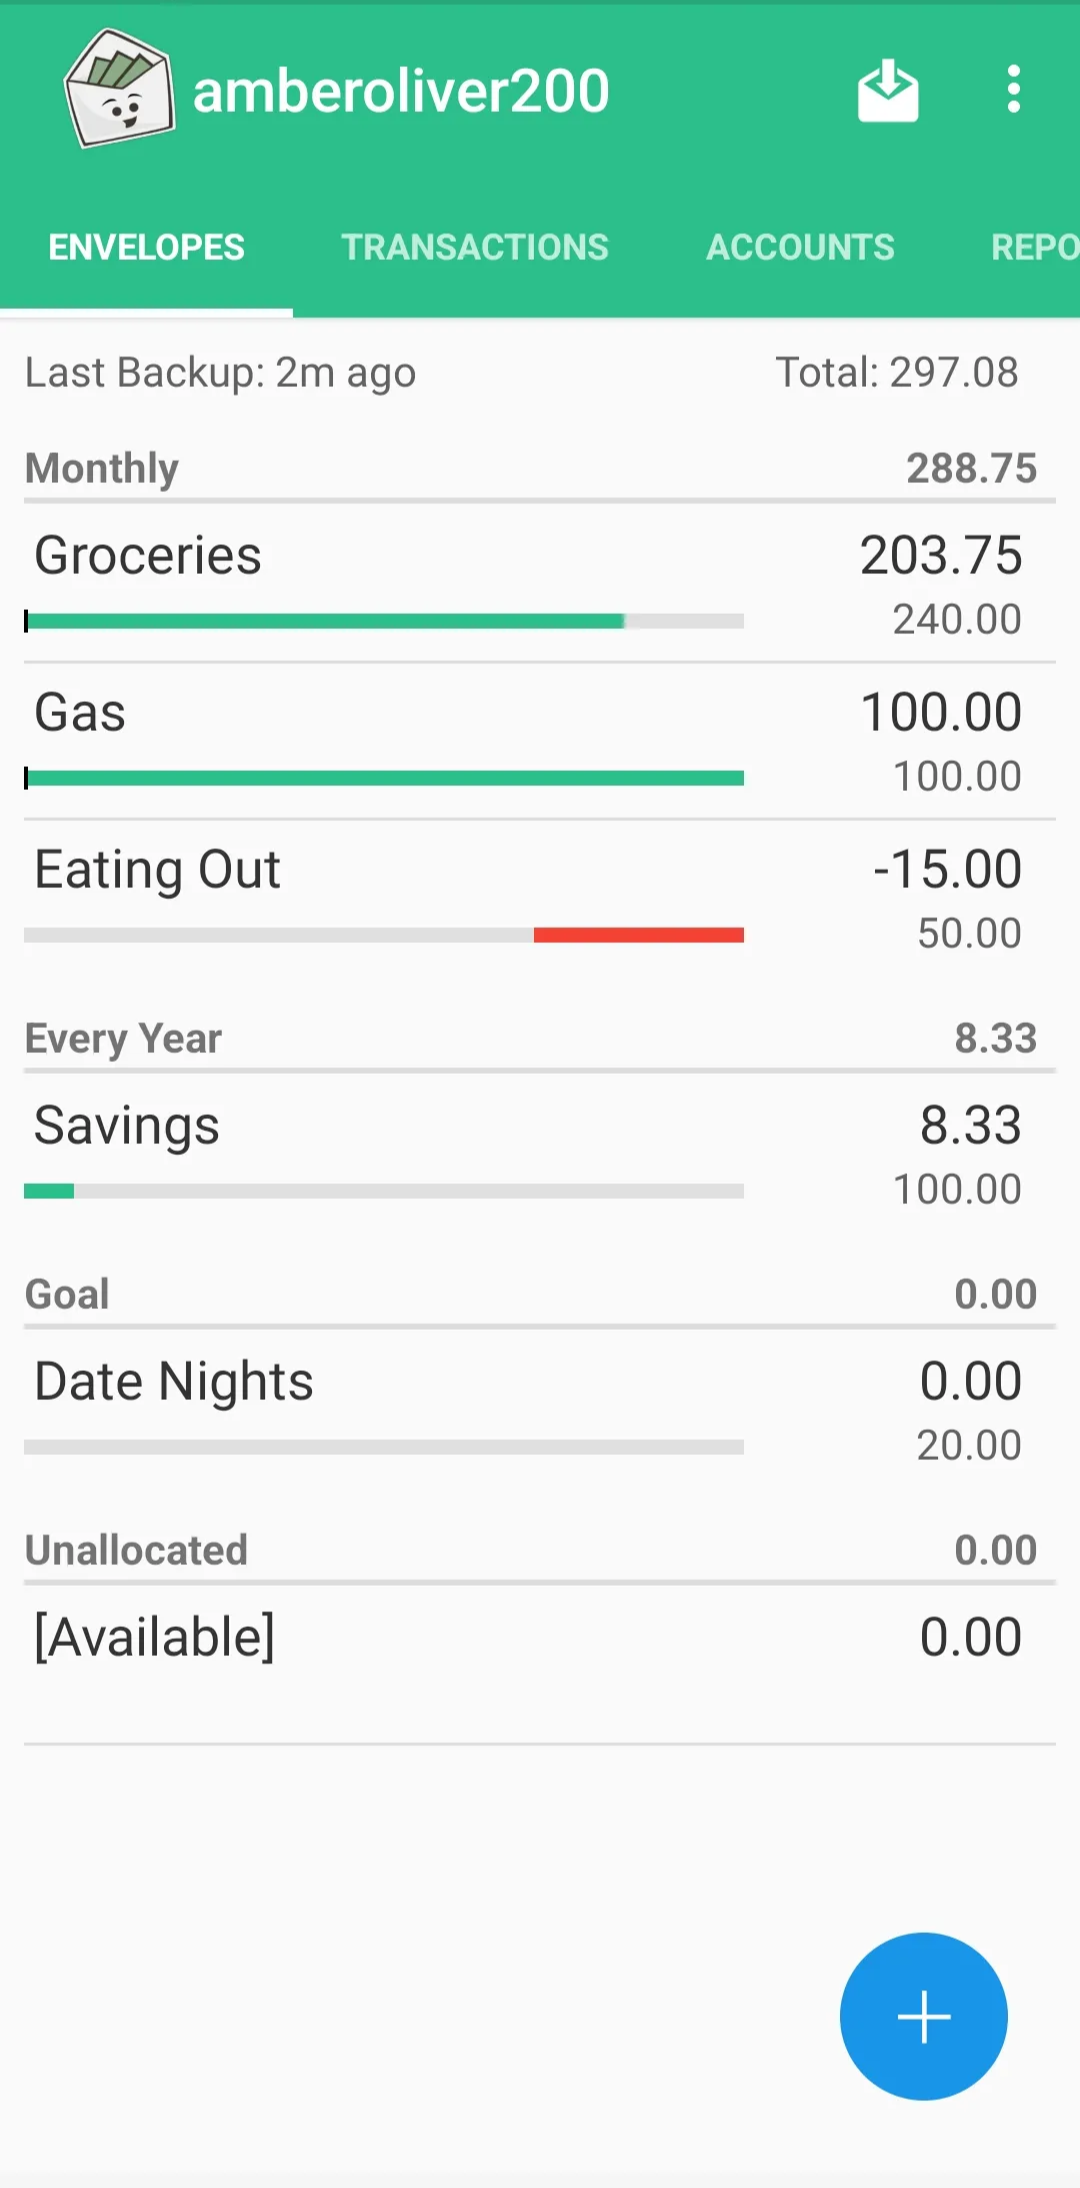
\includegraphics[width=\textwidth]{images/App-Comparison/goodbudget-ss-2.png}
        \caption{GoodBudget's Envelope Budgeting Implementation.}
        \label{fig:syn1}
    \end{subfigure}
    \hspace{0.5cm}
    \begin{subfigure}[t]{0.25\textwidth}
        \vspace{0pt}
        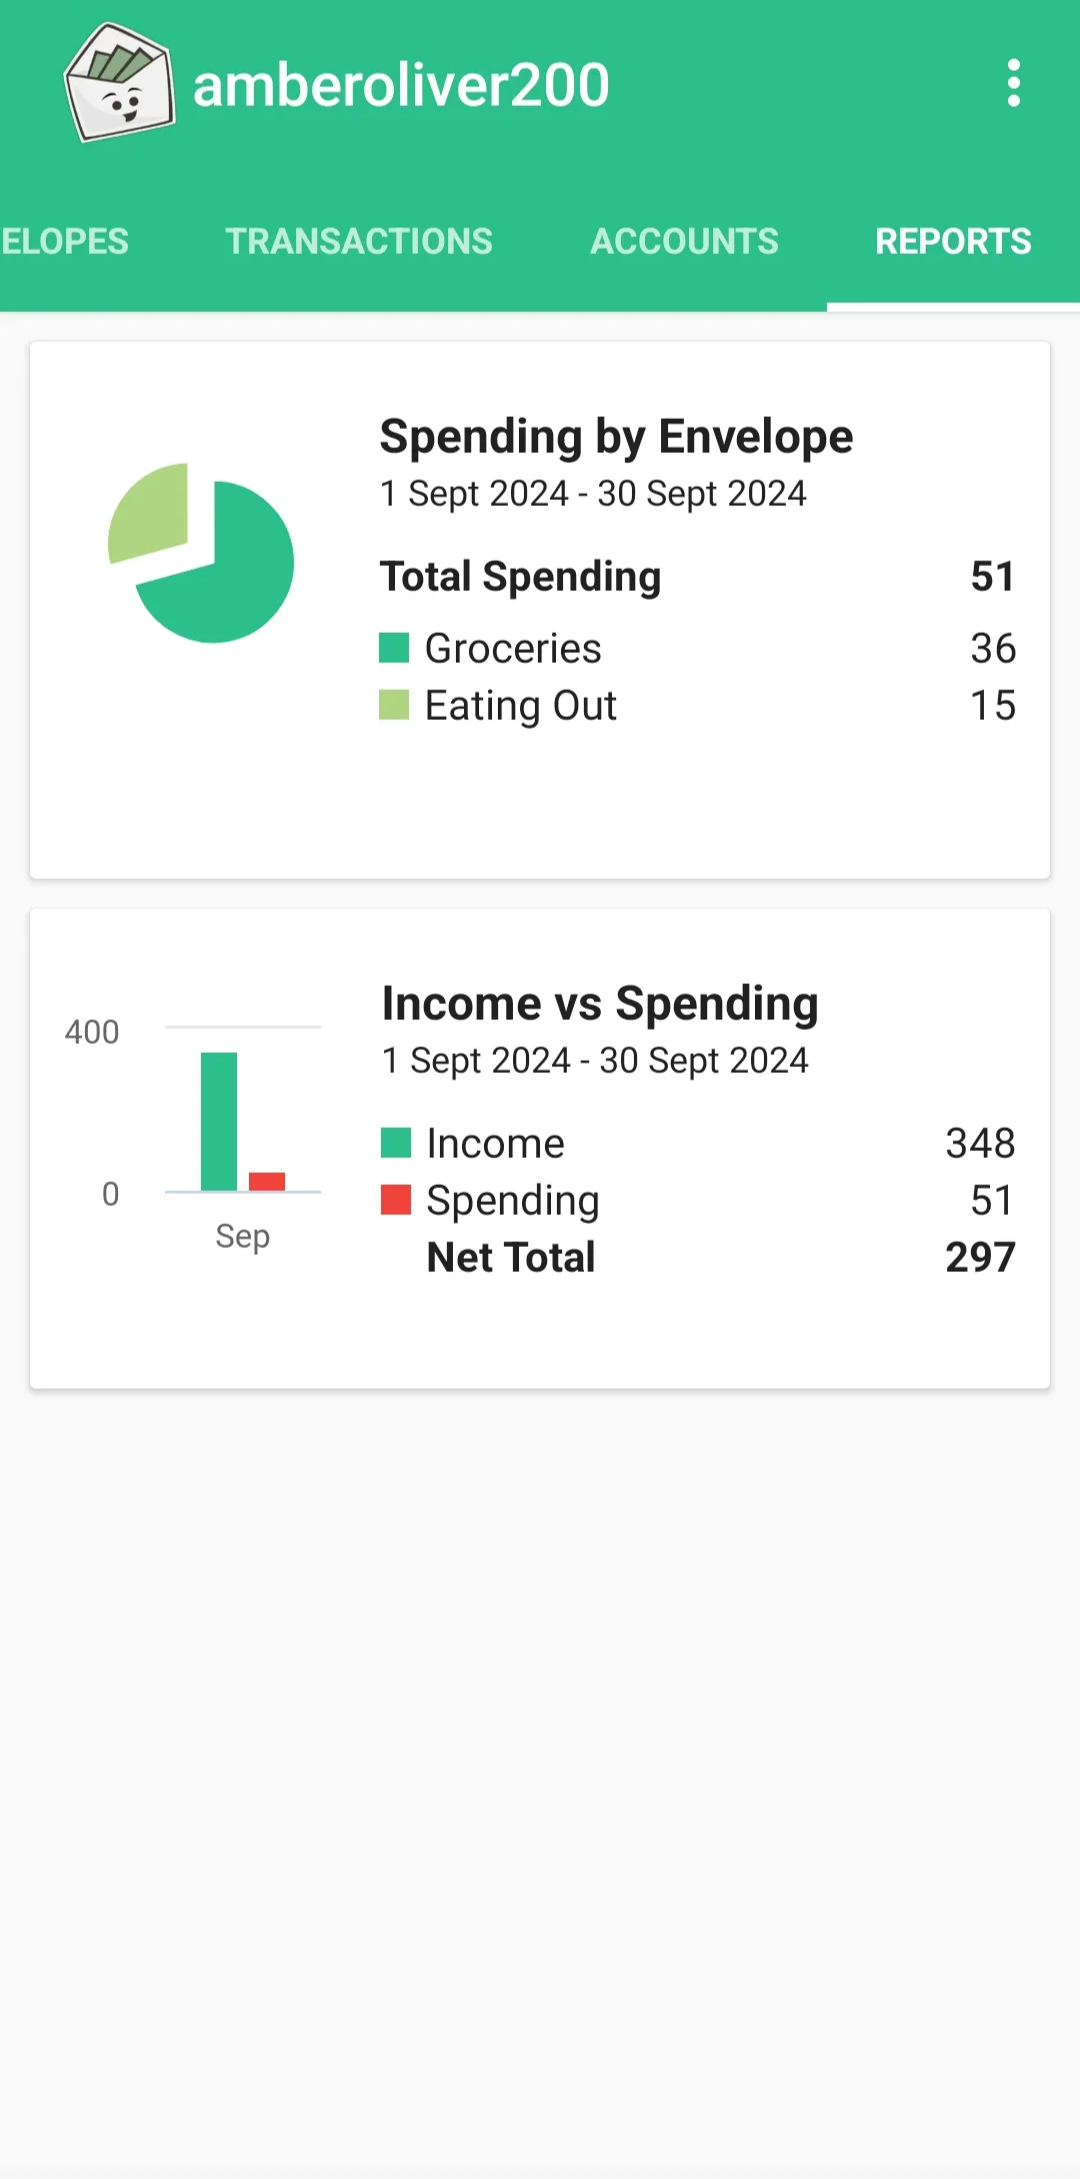
\includegraphics[width=\textwidth]{images/App-Comparison/goodbudget-ss-1.png} 
        \caption{GoodBudget's Report Page.}
        \label{fig:syn2}
    \end{subfigure}
    \caption{Screenshots of GoodBudget's UI. Progress bars can be seen for the amount spent of each envelope category in figure (a). Only 2 reports are available within the mobile app, as can be seen in (b).}
    \label{fig:synthetic}
\end{figure}

\section{Spending Tracker}

Spending Tracker is a manual-entry budgeting app that uses a blackboard-style UI to display income and expense categories and show how much has been spent in them. These values are then tallied up and displayed as the bank balance for that period. The app has no login, meaning the data is tied to the device. A one-time fee of £2.99 unlocks the paid version, which adds features like Dropbox sync, PDF export, priority support, and removes ads. While the budgeting concepts are simplistic, the UI can be confusing and limited.

\vspace{0.5em}
\textbf{Key features:}
\begin{itemize}
    \item Blackboard home page showing income and expense tallies for the selected period
    \item Manual entry of transactions, grouped into custom categories
    \item Multiple bank accounts supported, including transfers between accounts
    \item Transactions can be scheduled in advance and set to repeat (daily, weekly, or monthly)
    \item Basic reports and interactive charts (weekly, monthly, yearly)
    \item Budgeting goals showing leftover amounts carried into the next period
    \item CSV export (free) and PDF export with the paid version
    \item Dropbox backup and sync (paid feature)
\end{itemize}
\vspace{0.5em}

\textbf{Strengths/positive feedback (Google Play Store reviews):}
\begin{itemize}
    \item Simple to use, even without budgeting knowledge
    \item No limits on number of bank accounts or custom categories
    \item Scheduled transactions only affect the selected period, useful for “what if” planning
    \item One-off payment for Pro version is low-cost
    \item Does not require linking to a bank account
    \item Android users can back up data for free
\end{itemize}
\vspace{0.5em}

\textbf{Limitations/negative feedback (Google Play Store reviews):}
\begin{itemize}
    \item Best features are restricted to the paid version
    \item No login, data is device-specific
    \item Reports are limited to category breakdowns and cash flow only
    \item No way to show how a transaction was paid (e.g. card, transfer, etc)
    \item No income reports equivalent to the expenses charts
    \item Transactions sorted only by day with no way to change this
    \item No ability to assign budgets per category
    \item No payday-to-payday viewing option
    \item Dropbox is the only backup method, requiring a separate Dropbox account
\end{itemize}
\vspace{0.5em}

\textbf{Observations/personal experience:}
\begin{itemize}
    \item Switching between periods or adjusting the view date is not intuitive
    \item Reports page requires rotating the device, which is frustrating
    \item Budget mode must be manually enabled and is not clearly signposted
    \begin{itemize}
        \item The Budget mode only allows for a budget total to be entered so only applies to the overall balance, not individual categories
    \end{itemize}
    \item Ads are frequent and sometimes require watching 30-second videos
    \item While the app covers basic budgeting, it is almost too simplistic, offering little more than what a banking app already provides
    \item Useful for quick tracking, but lacks depth for long-term planning or goal-setting
\end{itemize}

\begin{figure}[h]
    \centering
    \begin{subfigure}[t]{0.25\textwidth}
        \vspace{0pt}
        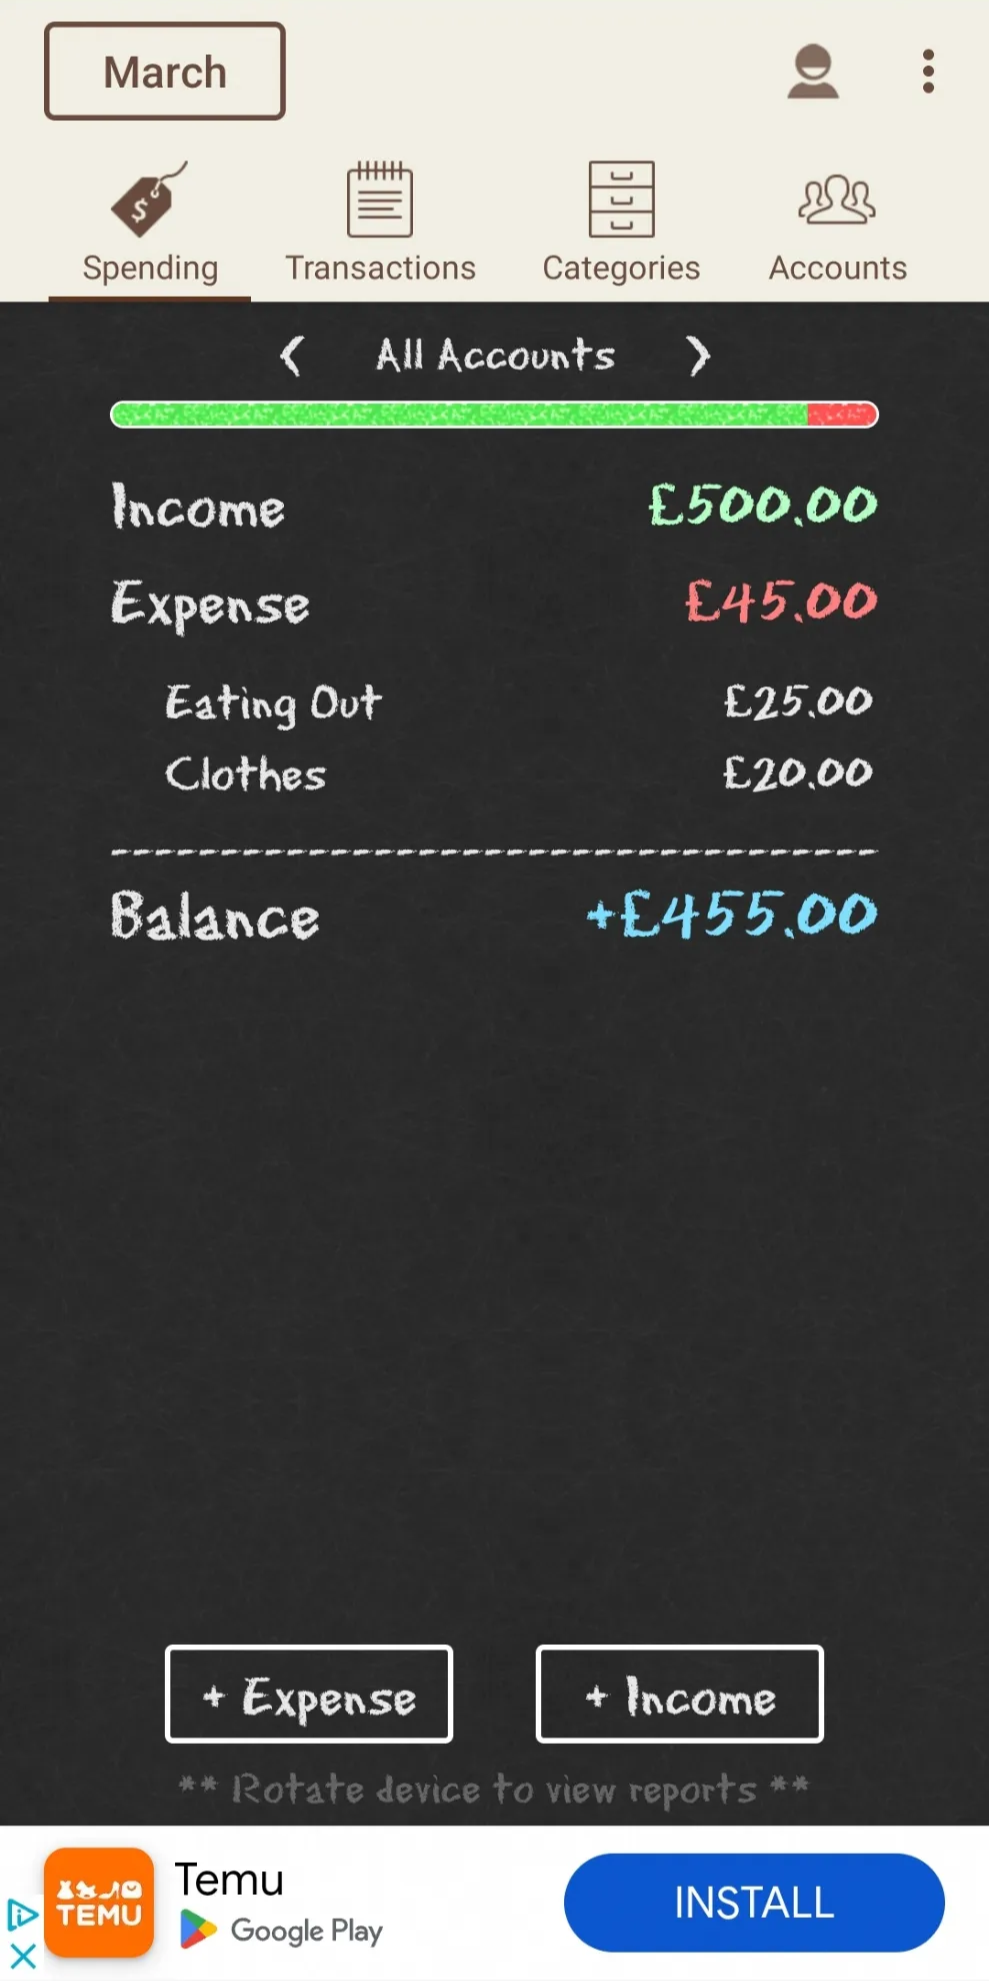
\includegraphics[width=\textwidth]{images/App-Comparison/spending-tracker-ss-1.png}
        \caption{Spending Tracker's Blackboard UI.}
        \label{fig:syn1}
    \end{subfigure}
    \hspace{0.5cm}
    \begin{subfigure}[t]{0.25\textwidth}
        \vspace{0pt}
        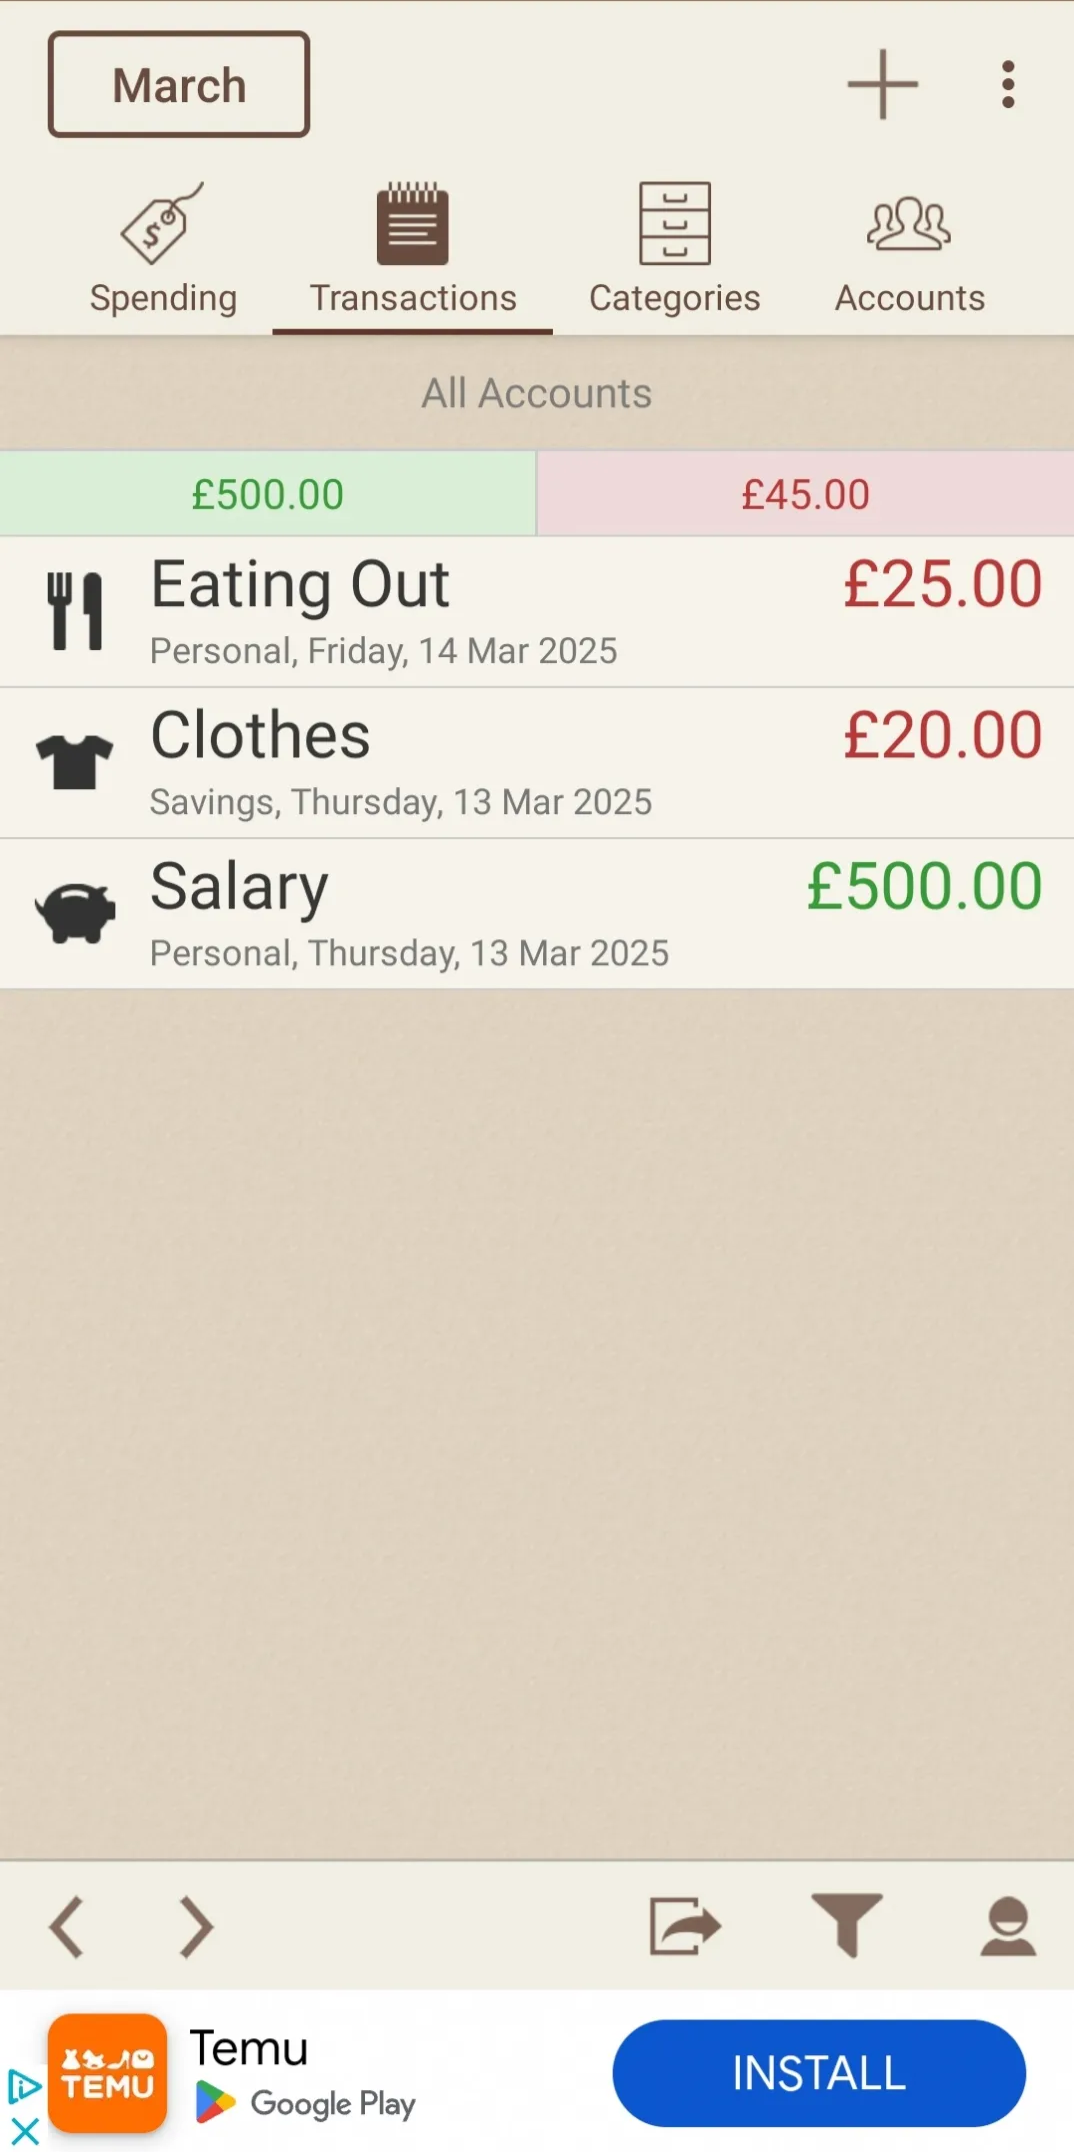
\includegraphics[width=\textwidth]{images/App-Comparison/spending-tracker-ss-2.png} 
        \caption{Spending Tracker's Transactions Page.}
        \label{fig:syn2}
    \end{subfigure}
    \caption{Screenshots of Spending Tracker's UI. Breakdown of spending in each category and income can be seen in (a). The amount spent and the category of each transaction can be seen in (b). Note that it is not possible to assign transactions names in this app.}
    \label{fig:synthetic}
\end{figure}

\section{Monefy}
Monefy is a manual-entry budgeting app that displays spending in a clear, category-based pie chart format. It allows quick tracking of where the user’s money is going by selecting a category and entering the amount spent. Transactions can be added either by choosing “Income”, “Expense”, or selecting a specific category directly.

The free version is limited, with key features locked behind a paywall. A subscription of £26.49 per year is required to unlock the full set of features, including repeated expenses, custom spending categories, login/sync functionality, and multi-device access.

\vspace{0.5em}
\textbf{Key features:}
\begin{itemize}
    \item Pie chart visualisation of expenses by category
    \item Add transactions by selecting “Income”, “Expense”, or a category directly
    \item View transactions either in pie chart form or as a list
    \item When adding a transaction: enter amount, note, category, and whether it is an income or expense
\end{itemize}
\vspace{0.5em}

\textbf{Strengths/positive points:}
\begin{itemize}
    \item Simple, visual layout makes it easy to understand where money is going
    \item Quick to enter transactions with minimal steps
    \item Clean and intuitive interface
\end{itemize}
\vspace{0.5em}

\textbf{Limitations/negative points:}
\begin{itemize}
    \item Most key features are locked behind a paywall (£26.49 per year)
    \item Cannot add recurring expenses without paying
    \item Custom categories are not available in the free version
    \item No login or sync options unless you pay
    \item Pie chart only displays expenses, not income
\end{itemize}

\begin{figure}[h]
    \centering
    \begin{subfigure}[t]{0.25\textwidth}
        \vspace{0pt}
        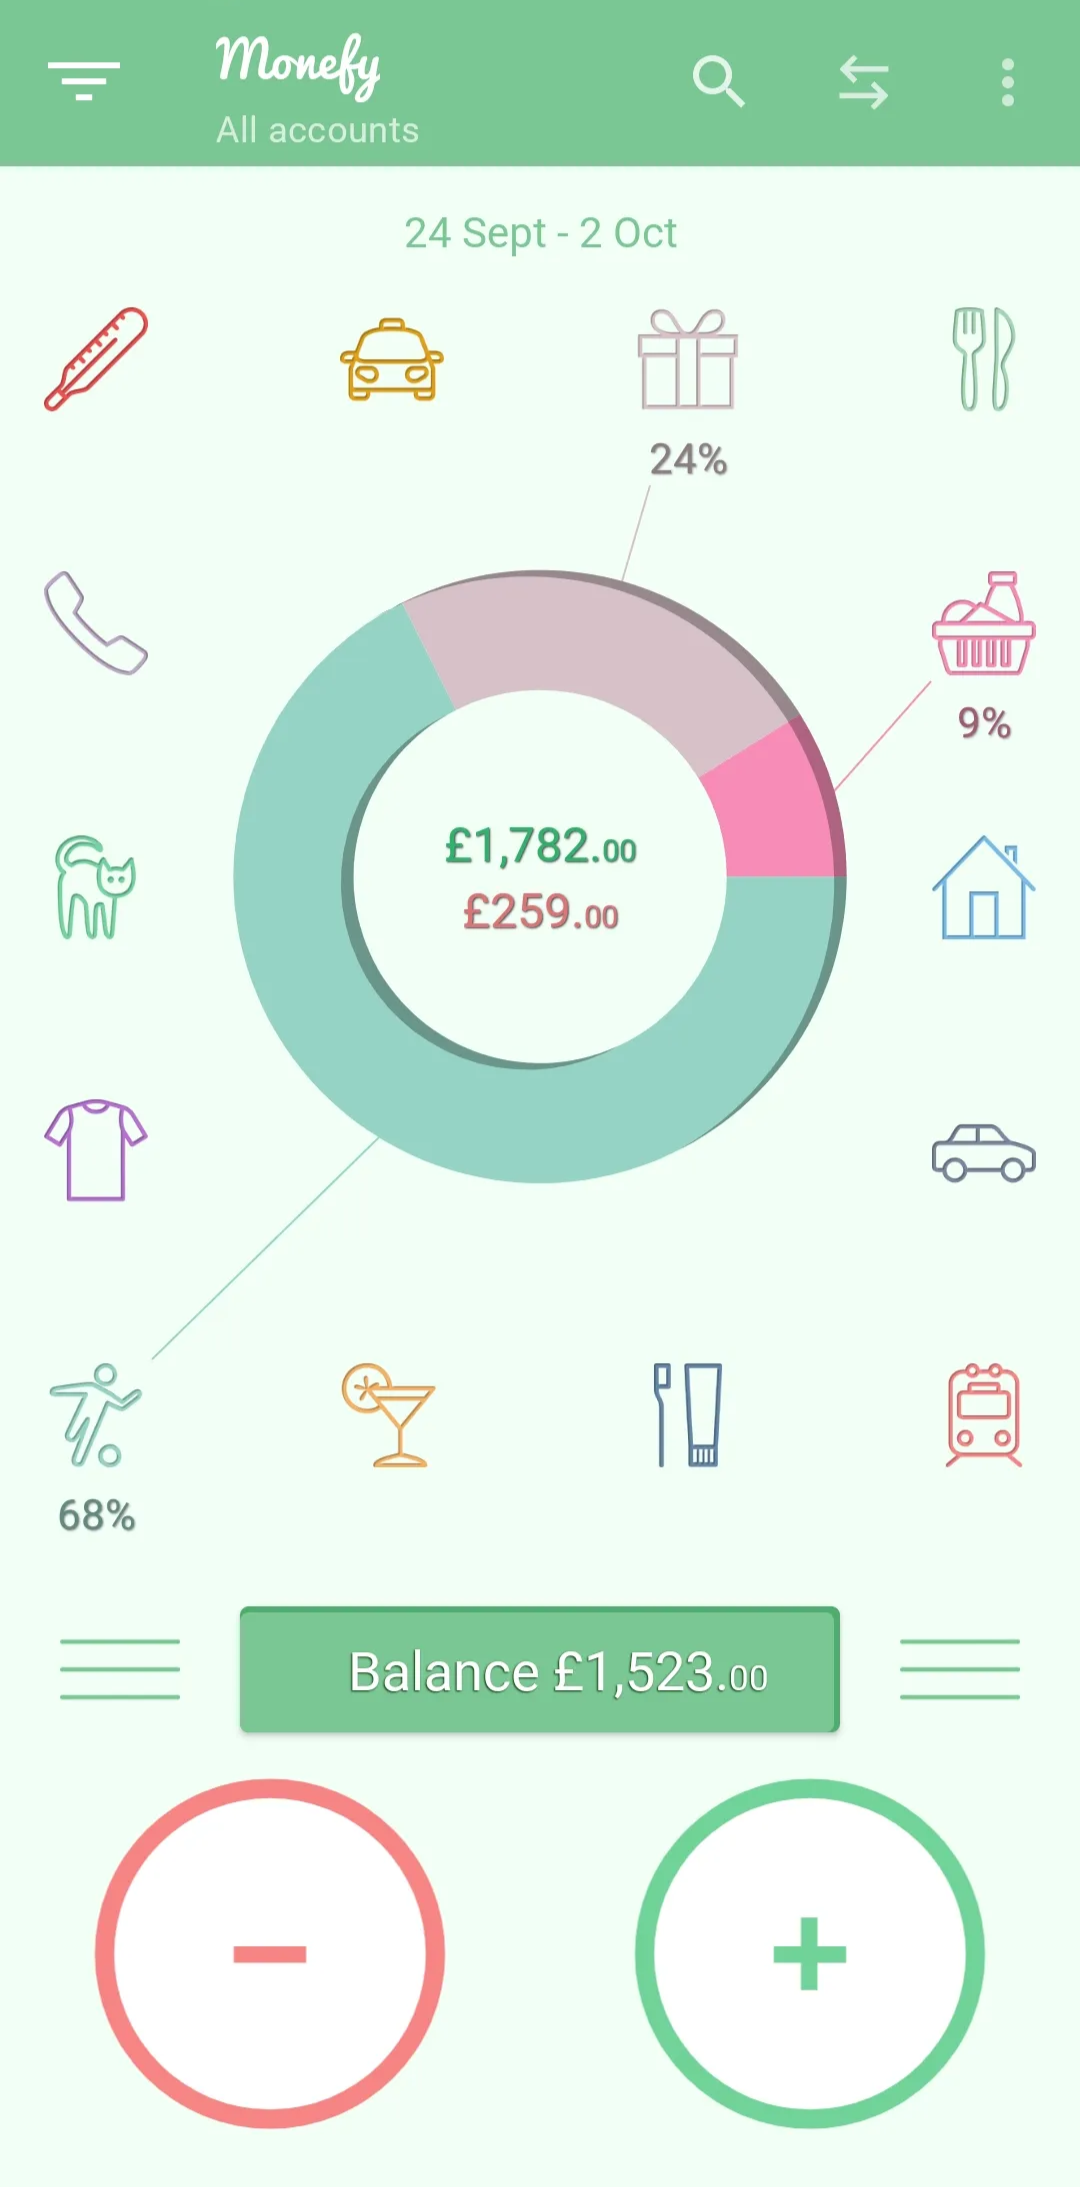
\includegraphics[width=\textwidth]{images/App-Comparison/monefy-ss-1.png}
        \caption{Monefy's Pie Chart Spending Breakdown.}
        \label{fig:syn1}
    \end{subfigure}
    \hspace{0.5cm}
    \begin{subfigure}[t]{0.25\textwidth}
        \vspace{0pt}
        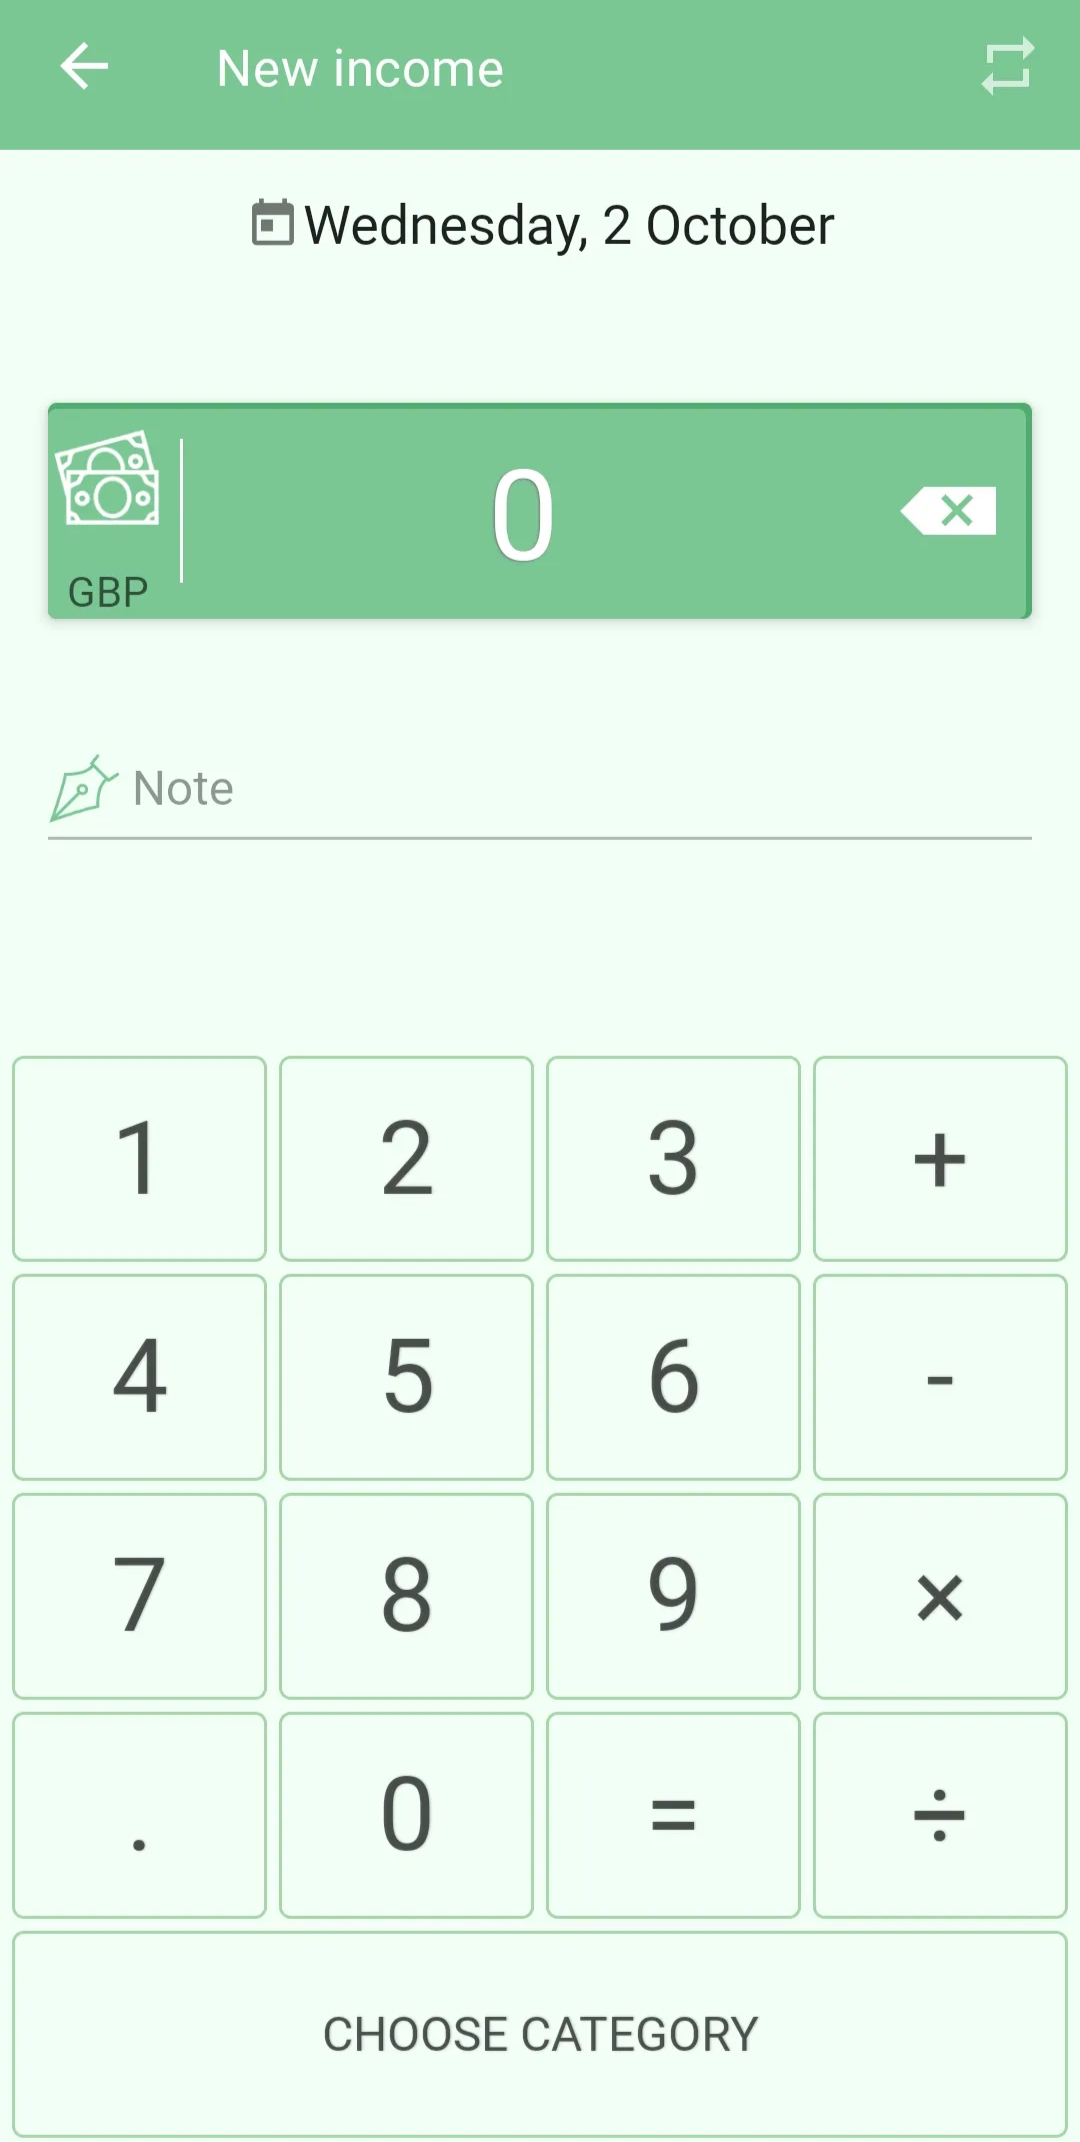
\includegraphics[width=\textwidth]{images/App-Comparison/monefy-ss-2.png} 
        \caption{Monefy's Add a Transaction Page.}
        \label{fig:syn2}
    \end{subfigure}
    \caption{Screenshots of Monefy's UI. Breakdown of spending in each category is displayed as a pie chart on the home page as seen in (a). To enter transactions, the user must use a built in calculator and can add very limited detail to the transaction, as can be seen in (b).}
    \label{fig:synthetic}
\end{figure}

\section{Budgeting Apps with Bank Account Integration}
Any app reviews mentioned can be found in Appendix \ref{app:reviews}.

\textbf{Snoop} was the first open banking budgeting app looked at. It integrates directly with users’ bank accounts to provide personalised insights and savings recommendations. By analysing spending data, Snoop offers tailored advice on how to save money, set financial goals, and improve overall financial health. It was found that while the app was easy to use, with a clean UI and interesting financial insights, it often categorised transactions incorrectly. This resulted in inaccurate insights and charts, meaning manual adjustments were needed for many transactions, even though one of the main points of linking a bank account is to reduce the need for manual input. A paid version is available, but it was found that most of the features interested in were accessible through the free version. Snoop is rated highly on the Google Play Store, with an average rating of 4.5. Many users appreciate that all key information is available in one place and that the interface is clear and easy to read. However, others also mentioned the inaccurate categorisation of transactions and the limited options for customisation of analytics and transaction information.

\textbf{PocketGuard} was the next app explored. It does not offer a free version, so the amount of the app available to be assessed was limited. From what could be seen, the app provides a simple and clear overview of spending and automatically categorises transactions through a bank account connection. Users can customise spending limits, receive a personalised debt payoff plan, and access resources to help manage their personal finances. However, with an average rating of 3.4 on the app store, reviews suggest that the bank connection is often unreliable, with users frequently having to reconnect their accounts. Others also mentioned slow syncing between their bank and the app, along with various glitches such as missing information and deleted transactions.

\textbf{YNAB (You Need a Budget)} uses a zero-based budgeting methodology, where users assign every dollar or pound to a specific expense at the start of the month. The app connects to bank accounts and syncs across multiple devices. Although there is no free version, a YNAB subscription can be shared across multiple users, which makes it more cost-effective for couples, families, or housemates. In addition to core budgeting features, YNAB provides loan calculators, spending and net worth reports, and a range of financial help guides. The app is rated very highly on the Google Play Store, with an average rating of 4.9. Despite this, there are recurring criticisms, including the high subscription cost, the inability to rename transactions (which default to the payment processor’s name), and the steep learning curve, as the zero-based budgeting method is not always intuitive to new users.

\textbf{Rocket Money} is a budgeting app with a specific focus on managing subscriptions and recurring payments. It aggregates bank account data to provide insights into spending trends and offers tools to help users cancel unwanted subscriptions and negotiate bills. Rocket Money even provides negotiators who will contact service providers on the user’s behalf to try to reduce bills, and it also offers its own credit card with a focus on building mortgage savings. A free version of the app is available, along with a premium version that unlocks additional features such as subscription cancellation services, account sharing, and full credit reports. However, Rocket Money is not currently available in the UK or for users with UK-based bank accounts.

\chapter{App Store Reviews of Existing Budgeting Apps}
\label{app:reviews}
\section{GoodBudget Reviews}
\textbf{Positive Reviews:}
\begin{figure}[H]
    \centering
    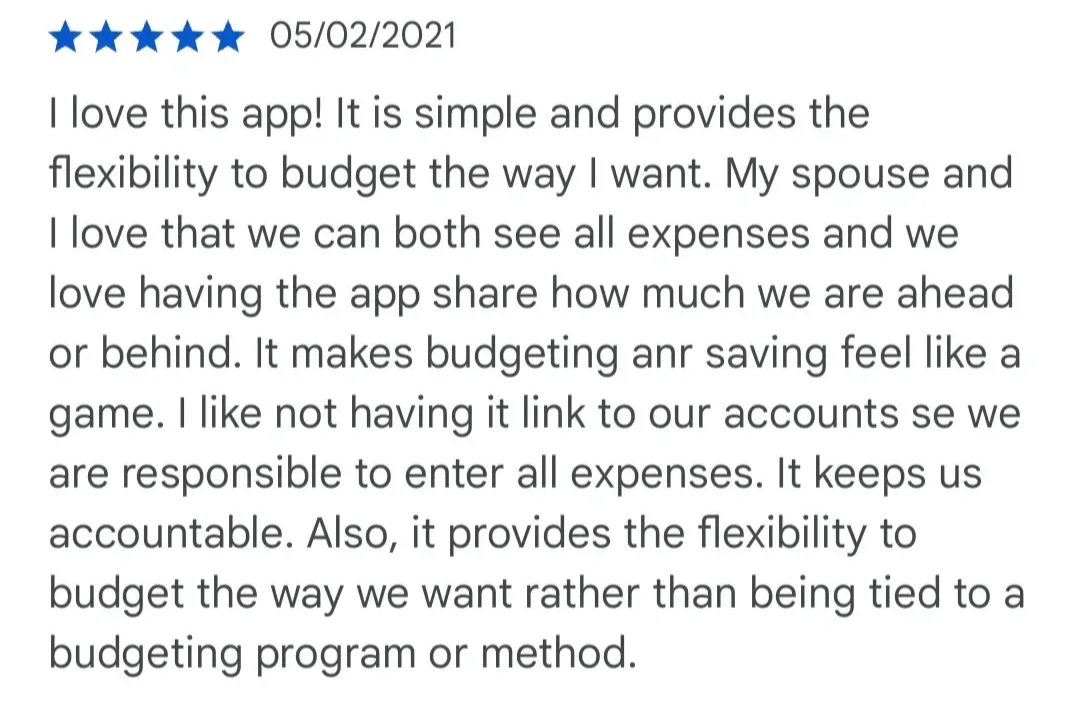
\includegraphics[width=0.5\linewidth]{images/App-Comparison/goodbudget-pos-1.png}
    \caption{Review that mentions how they like manually entering transactions as it holds them accountable for their spending.}
    \label{fig:enter-label}
\end{figure}
\begin{figure}[H]
    \centering
    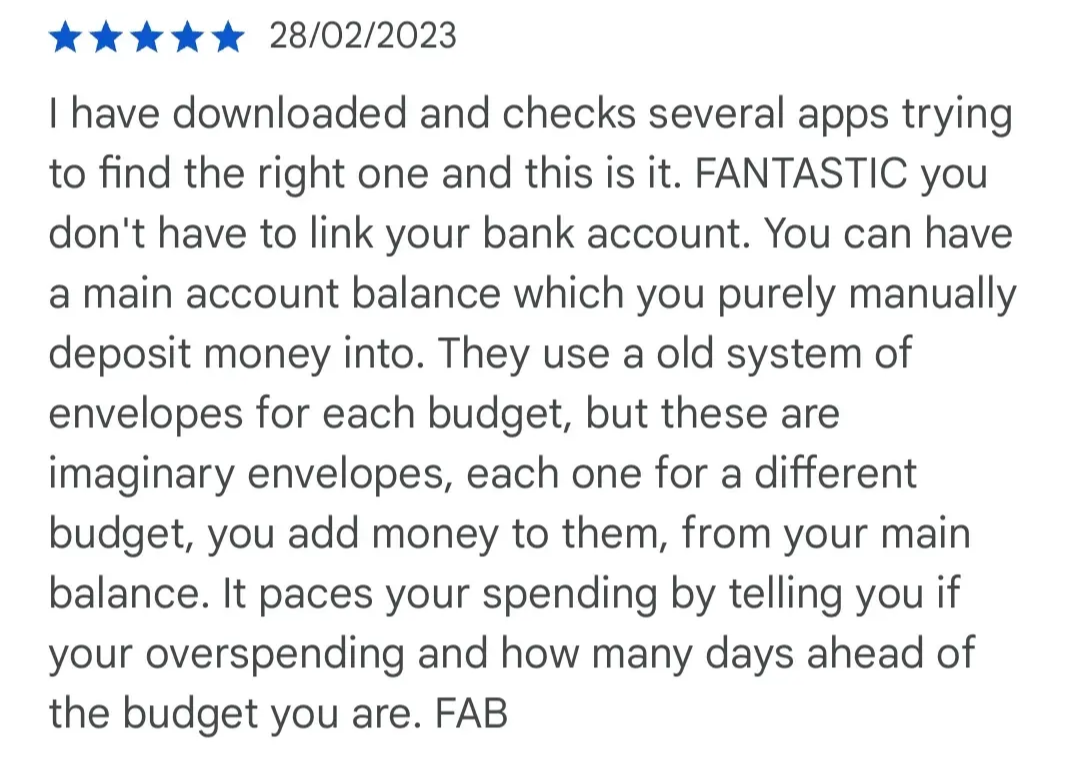
\includegraphics[width=0.5\linewidth]{images/App-Comparison/goodbudget-pos-2.png}
    \caption{Review that mentions how they like that the app does not require them to link their bank account and that they like the envelope system.}
    \label{fig:enter-label}
\end{figure}
\begin{figure}[H]
    \centering
    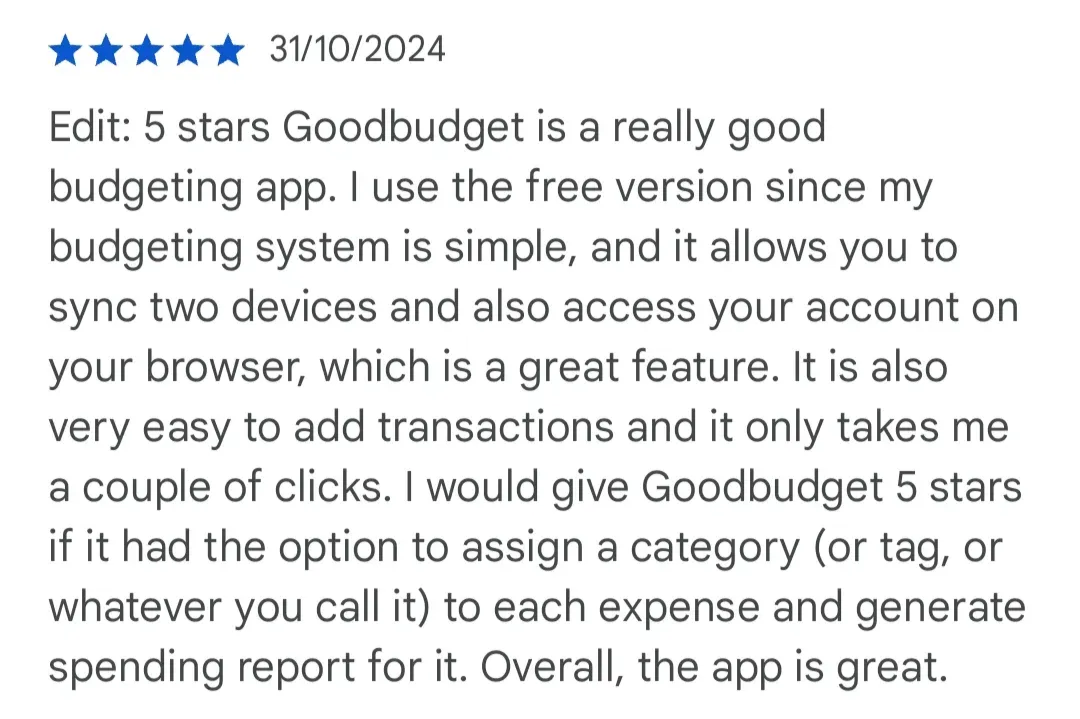
\includegraphics[width=0.5\linewidth]{images/App-Comparison/goodbudget-pos-3.png}
    \caption{Review that mentions how they like that they can sync across devices but does not like that reporting is so rigid.}
    \label{fig:enter-label}
\end{figure}

\textbf{Negative Reviews:}
\begin{figure}[H]
    \centering
    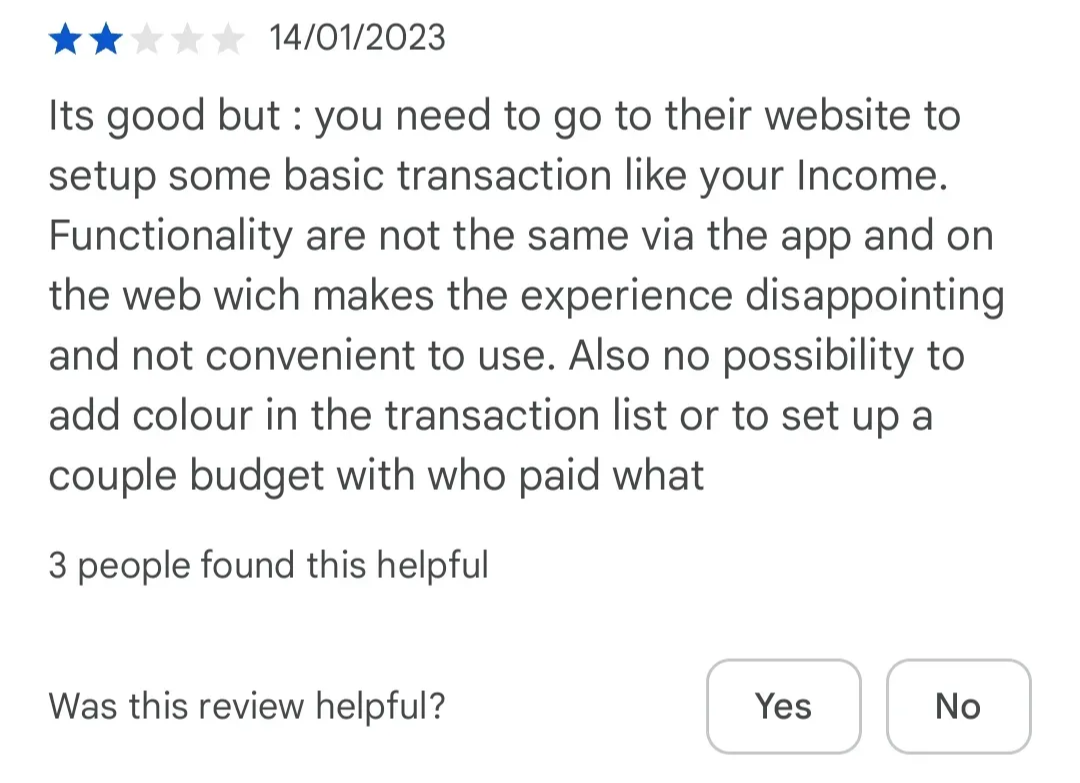
\includegraphics[width=0.5\linewidth]{images/App-Comparison/goodbudget-neg-1.png}
    \caption{Review that mentions the lack of consistency between the mobile and web app.}
    \label{fig:enter-label}
\end{figure}
\begin{figure}[H]
    \centering
    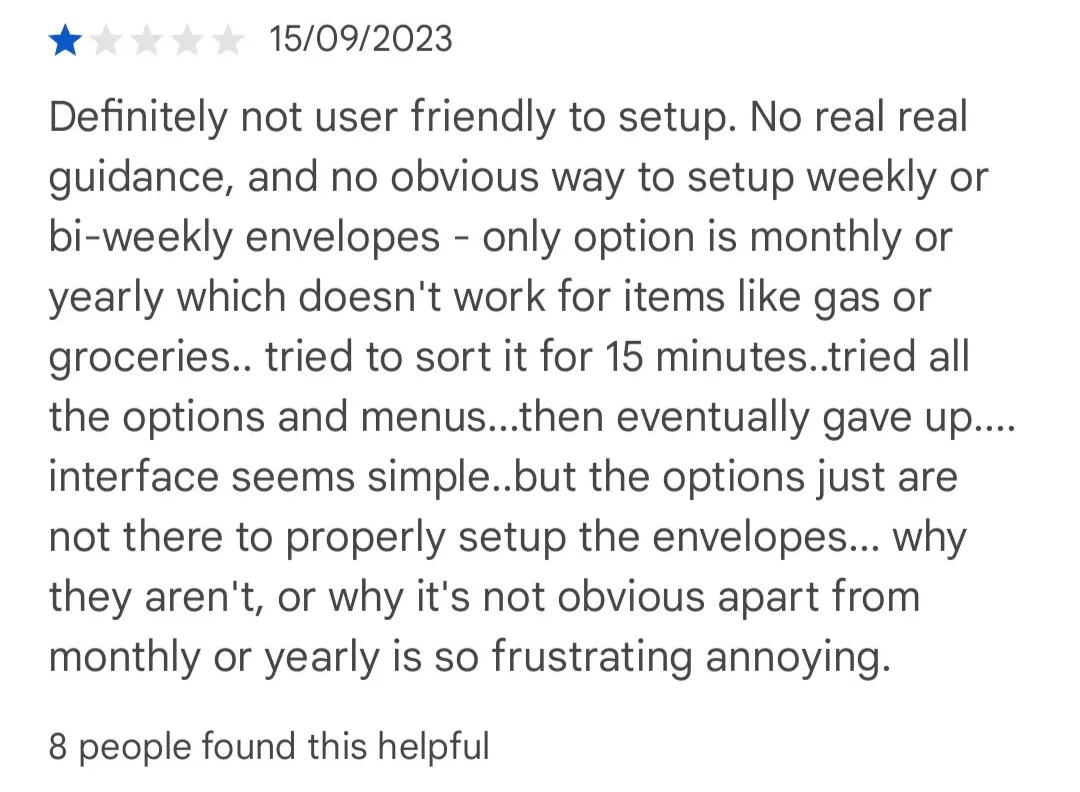
\includegraphics[width=0.5\linewidth]{images/App-Comparison/goodbudget-neg-2.png}
    \caption{Review that mentions the lack of repeat periods for repeated transactions.}
    \label{fig:enter-label}
\end{figure}
\begin{figure}[H]
    \centering
    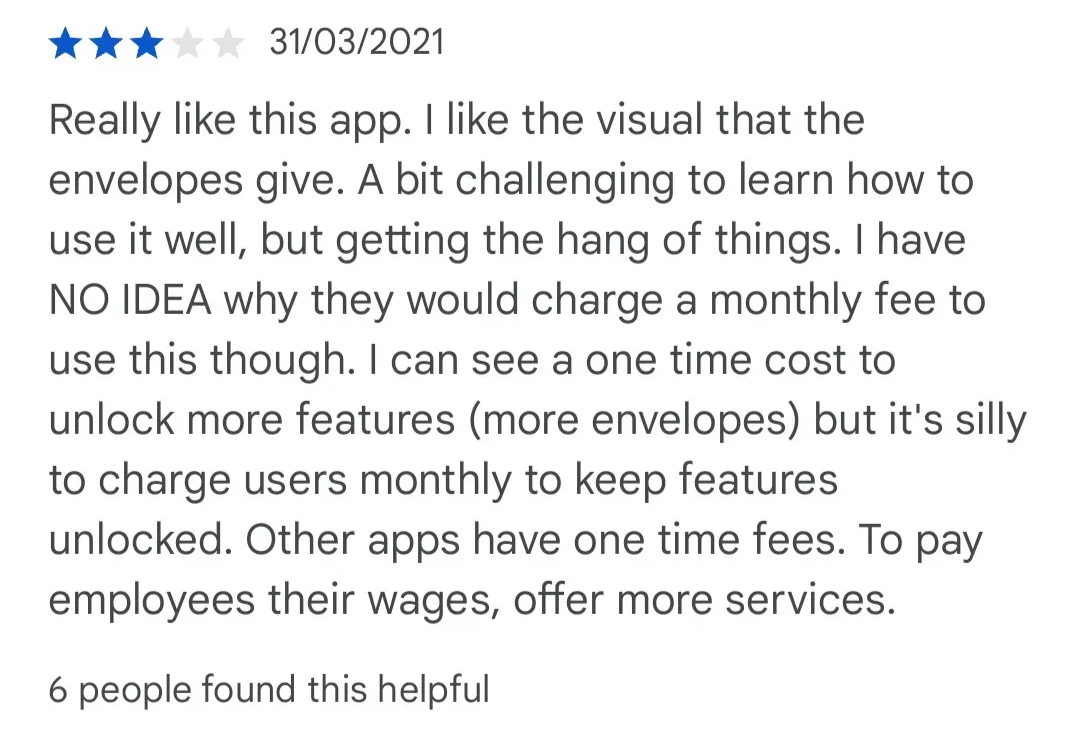
\includegraphics[width=0.5\linewidth]{images/App-Comparison/goodbudget-neg-3.png}
    \caption{Review that complains about the price but they like the envelope approach.}
    \label{fig:enter-label}
\end{figure}

\section{Spending Tracker Reviews}
\begin{figure}[H]
    \centering
    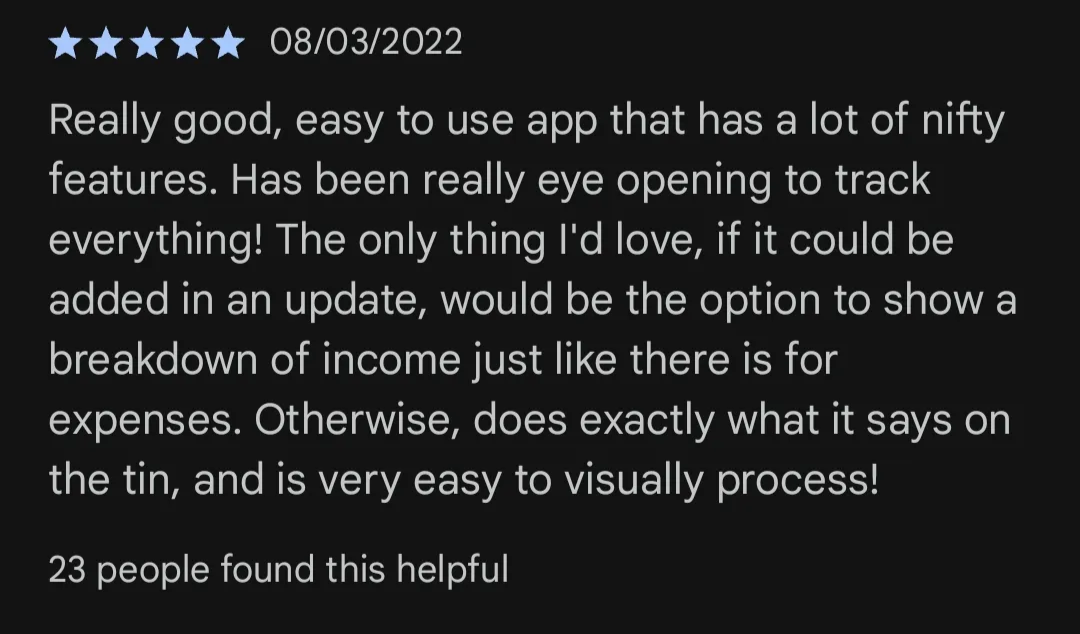
\includegraphics[width=0.5\linewidth]{images/App-Comparison/spending-tracker-review-1.png}
    \caption{Review talking about how the app does not have income reports and breakdowns.}
    \label{fig:enter-label}
\end{figure}
\begin{figure}[H]
    \centering
    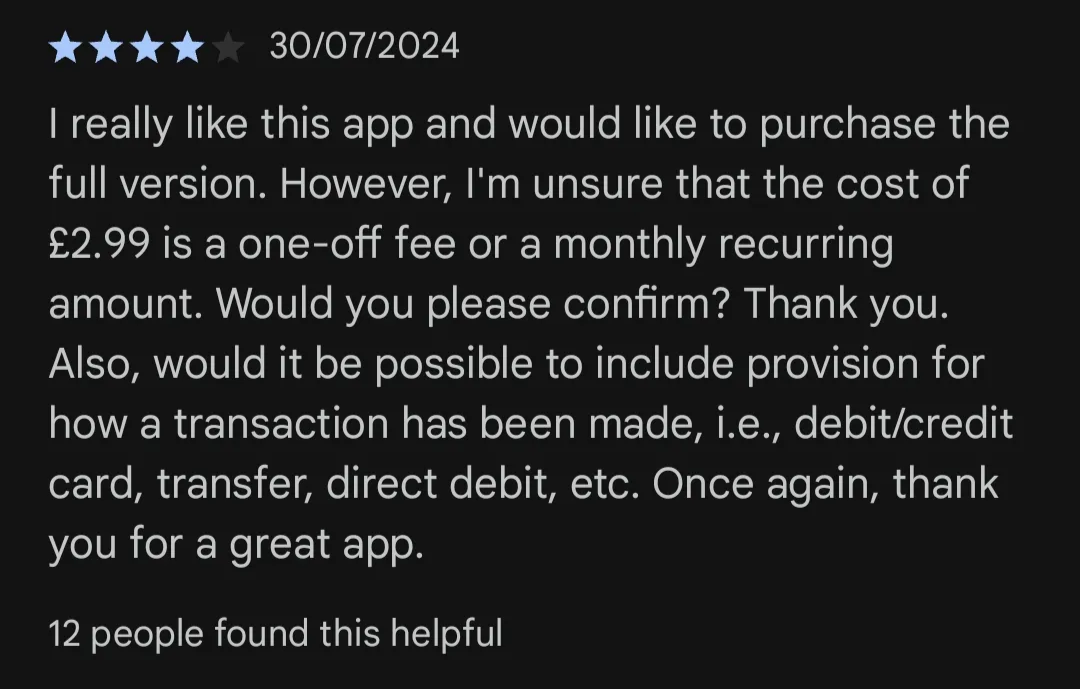
\includegraphics[width=0.5\linewidth]{images/App-Comparison/spending-tracker-review-2.png}
    \caption{Review talking about how the user would like to be able to add a payment type detail to transactions.}
    \label{fig:enter-label}
\end{figure}
\begin{figure}[H]
    \centering
    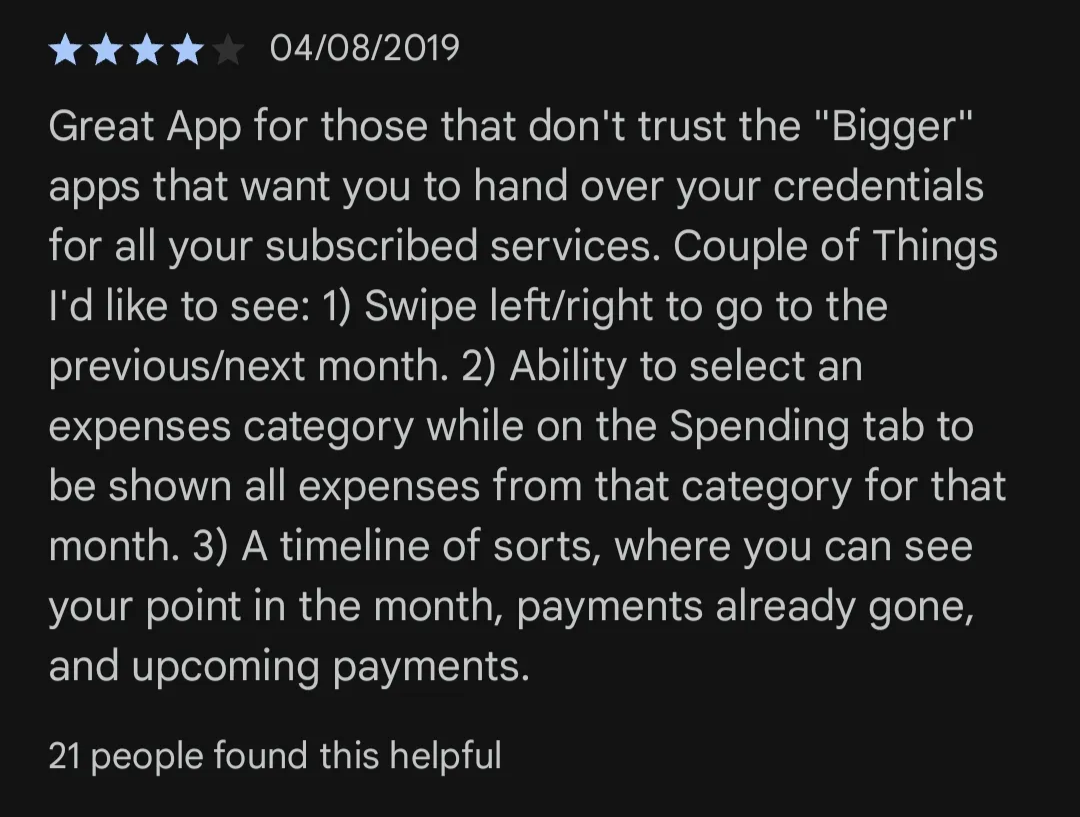
\includegraphics[width=0.5\linewidth]{images/App-Comparison/spending-tracker-review-3.png}
    \caption{Review that mentions the user likes that they do not have to share their personal details or connect their bank account in order to use the app.}
    \label{fig:enter-label}
\end{figure}

\begin{figure}[H]
    \centering
    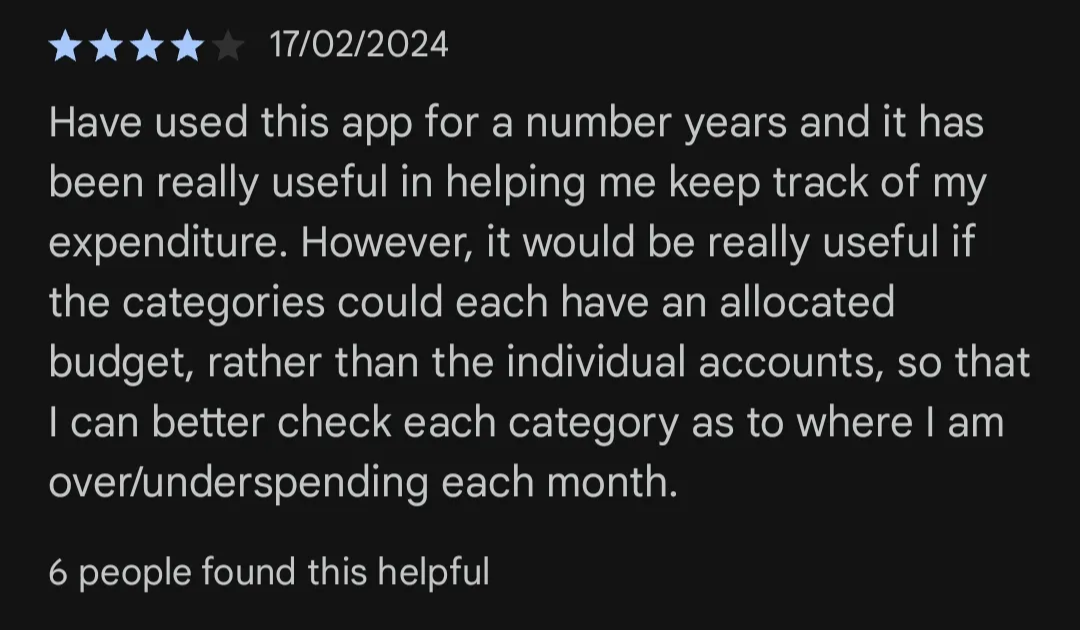
\includegraphics[width=0.5\linewidth]{images/App-Comparison/spending-tracker-review-4.png}
    \caption{Review that mentions the inability to set budget limits for specific categories.}
    \label{fig:enter-label}
\end{figure}
\begin{figure}[H]
    \centering
    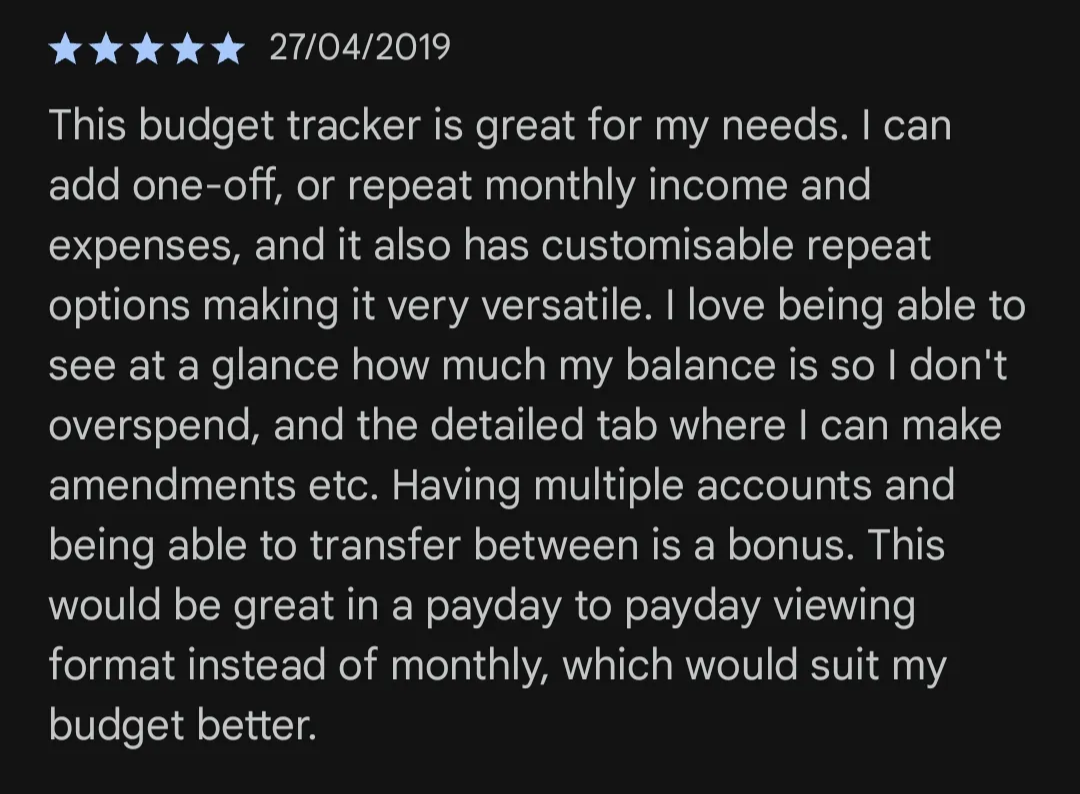
\includegraphics[width=0.5\linewidth]{images/App-Comparison/spending-tracker-review-5.png}
    \caption{Review that talks about how the user liked being able to track multiple bank accounts but that they would like to have a payday-to-payday financial period. Also mentions how they like how customisable the repeat periods are.}
    \label{fig:enter-label}
\end{figure}
\begin{figure}[H]
    \centering
    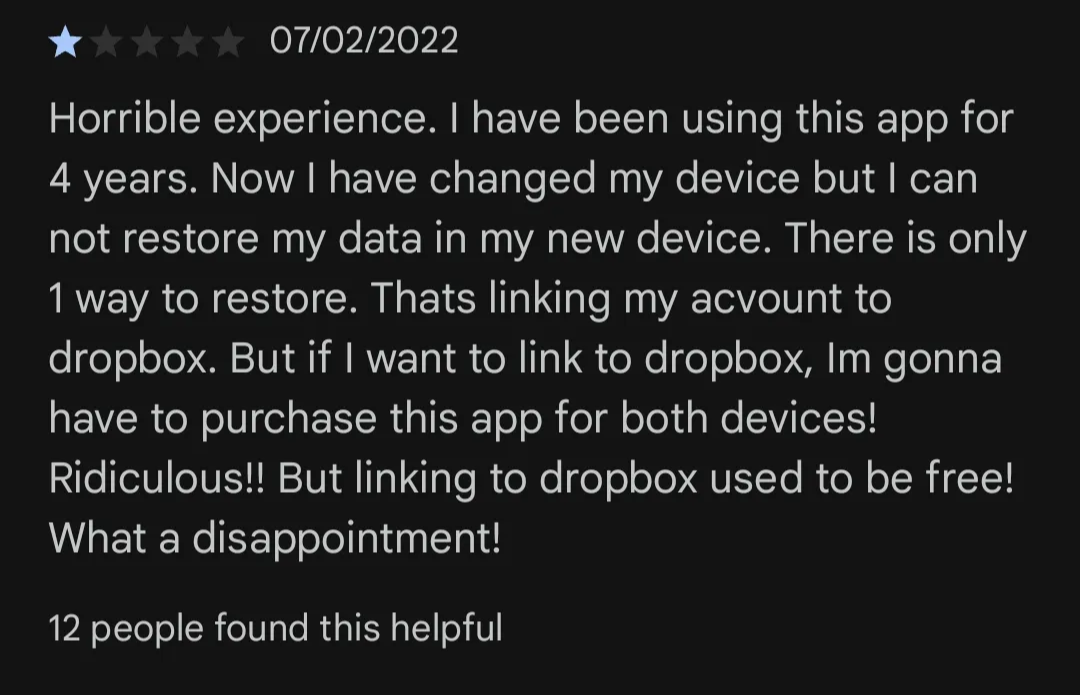
\includegraphics[width=0.5\linewidth]{images/App-Comparison/spending-tracker-review-6.png}
    \caption{Review that complains about how you must use Dropbox in order to save data. Also mentions how if you pay for the pro version of the app, you need to pay for it on every device you use the app due to the lack of login.}
    \label{fig:enter-label}
\end{figure}
\begin{figure}[H]
    \centering
    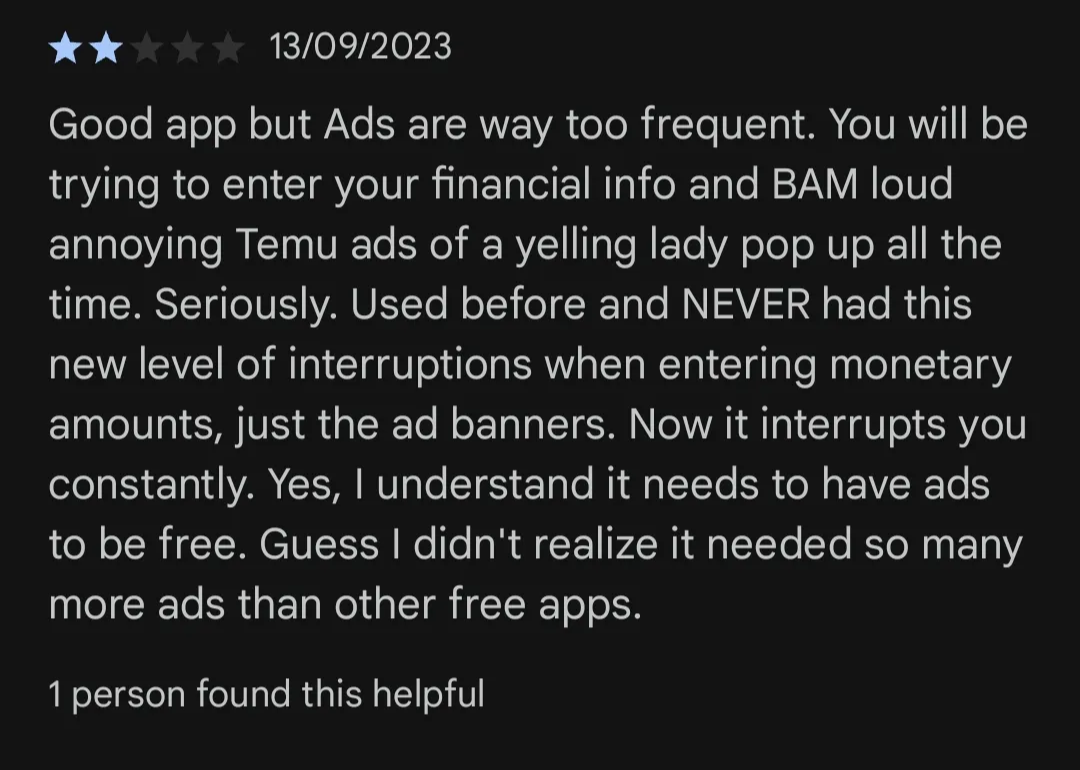
\includegraphics[width=0.5\linewidth]{images/App-Comparison/spending-tracker-review-7.png}
    \caption{Review that complains about the amount and frequency of ads in the app.}
    \label{fig:enter-label}
\end{figure}

\section{Snoop Reviews}
\begin{figure}[H]
    \centering
    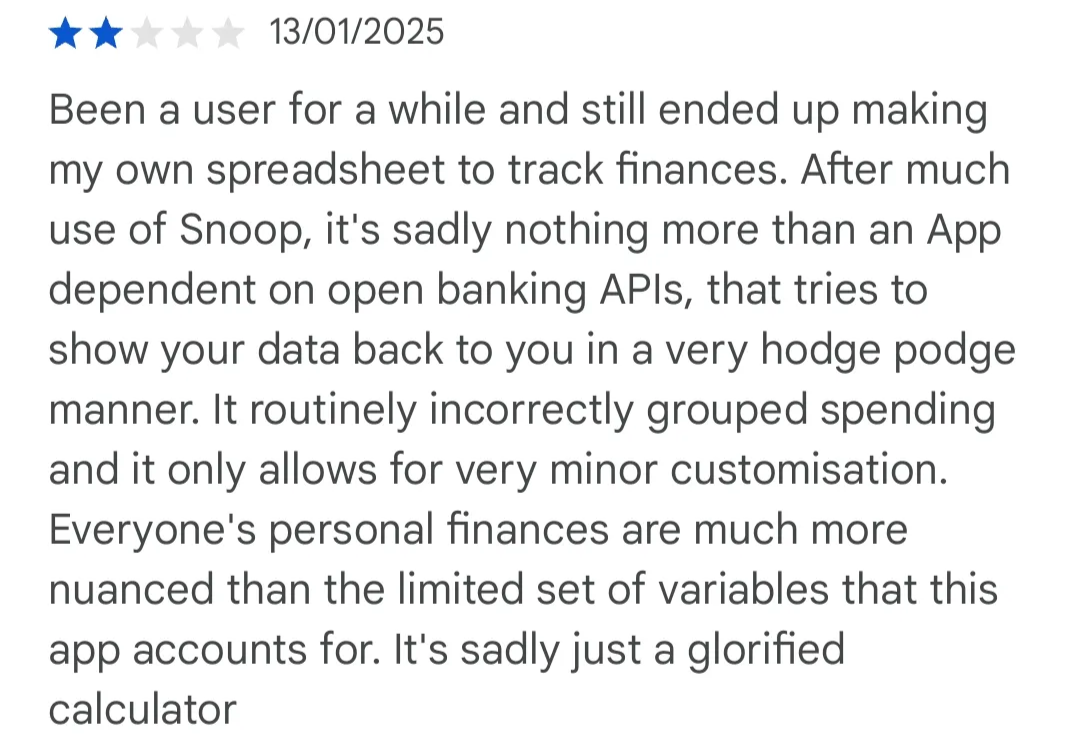
\includegraphics[width=0.5\linewidth]{images/App-Comparison/snoop-review-1.png}
    \caption{Review discussing how transactions are often miscategorised and how the app allows very little customisation.}
    \label{fig:enter-label}
\end{figure}
\begin{figure}[H]
    \centering
    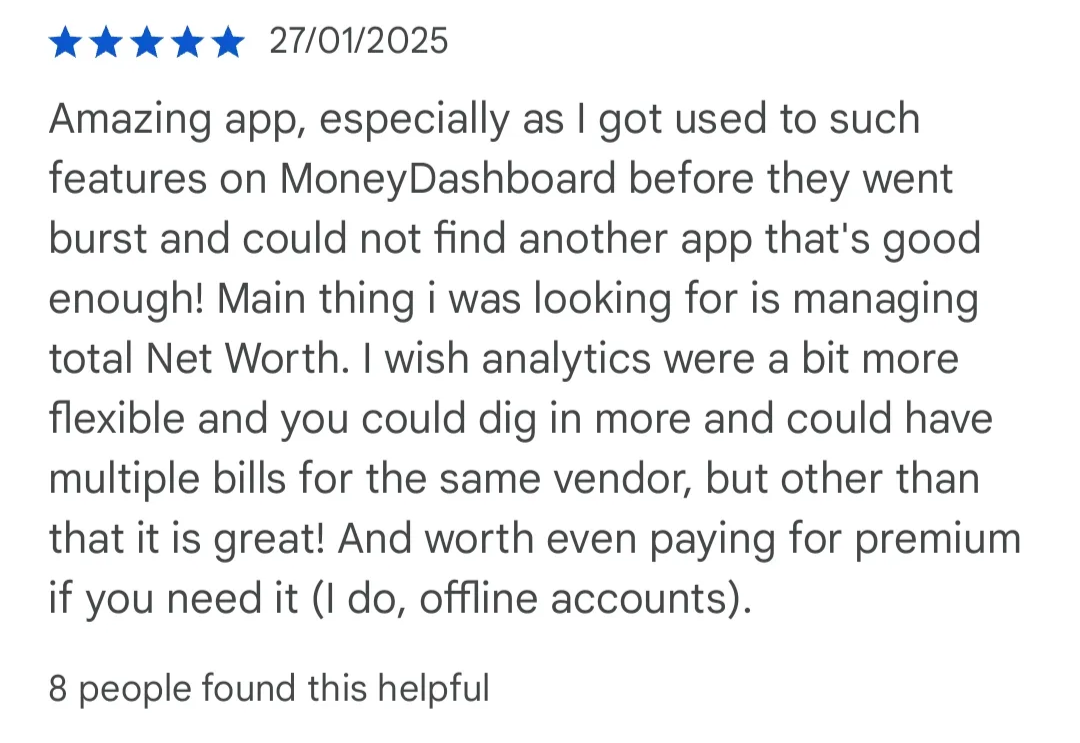
\includegraphics[width=0.5\linewidth]{images/App-Comparison/snoop-review-2.png}
    \caption{Review talking about how the analytics and reports are rigid.}
    \label{fig:enter-label}
\end{figure}
\begin{figure}[H]
    \centering
    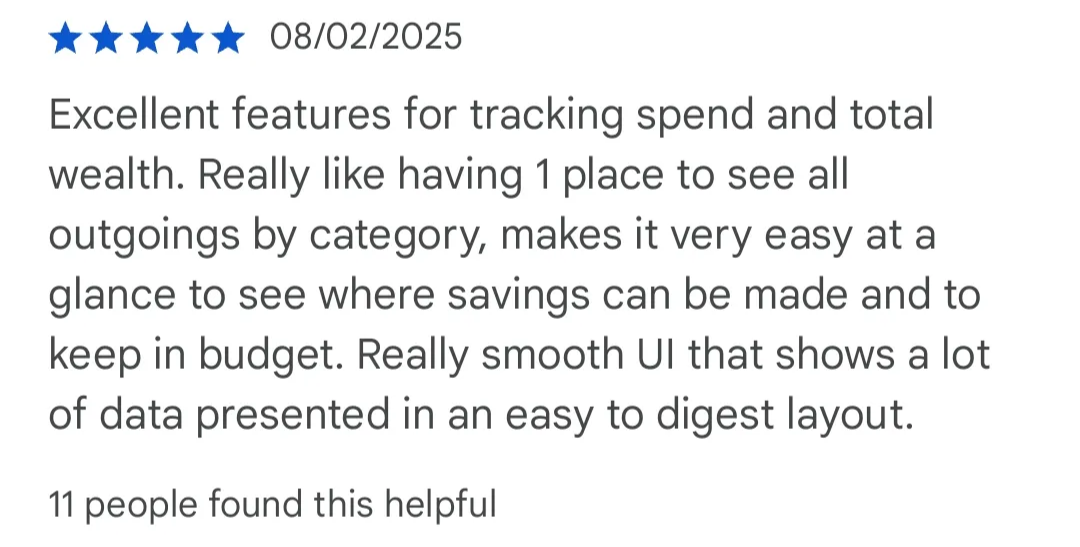
\includegraphics[width=0.5\linewidth]{images/App-Comparison/snoop-review-3.png}
    \caption{Review discussing how having all information in one place is really helpful and that the UI is clear and easy to use.}
    \label{fig:enter-label}
\end{figure}

\section{PocketGuard Reviews}
\begin{figure}[H]
    \centering
    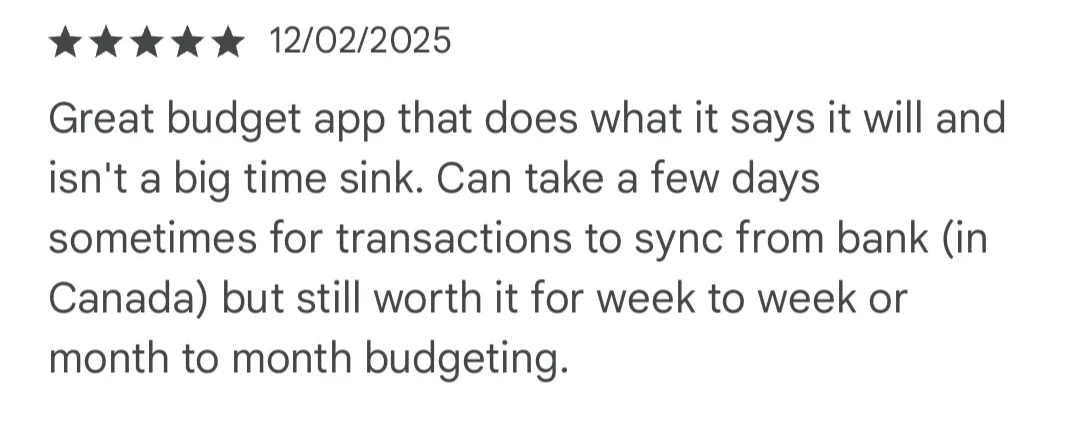
\includegraphics[width=0.5\linewidth]{images/App-Comparison/pocket-guard-review-2.png}
    \caption{Review complaining how the app’s link with bank accounts often disconnects. Also discusses loss of transactions and data when cards are cancelled.}
    \label{fig:enter-label}
\end{figure}
\begin{figure}[H]
    \centering
    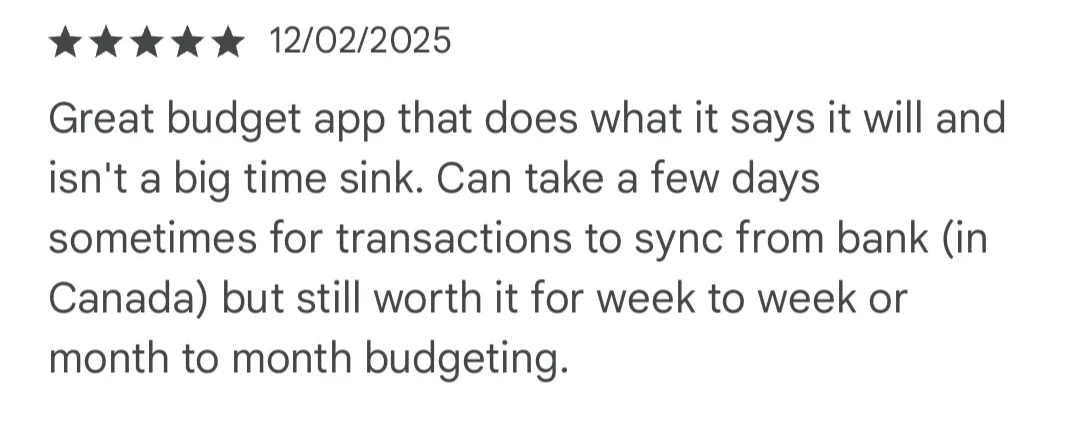
\includegraphics[width=0.5\linewidth]{images/App-Comparison/pocket-guard-review-2.png}
    \caption{Review talking about how syncing data from the bank account can be slow.}
    \label{fig:enter-label}
\end{figure}

\section{YNAB Reviews}
\begin{figure}[H]
    \centering
    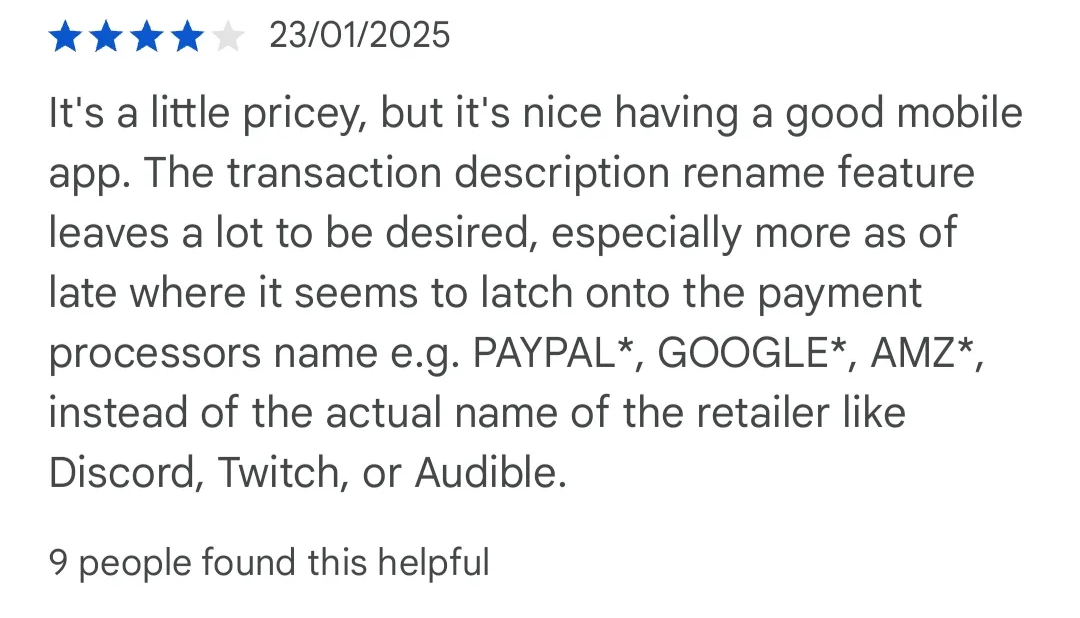
\includegraphics[width=0.5\linewidth]{images/App-Comparison/ynab-review-1.png}
    \caption{Review talking about how the app is expensive and how you cannot change the name of transactions.}
    \label{fig:enter-label}
\end{figure}
\begin{figure}[H]
    \centering
    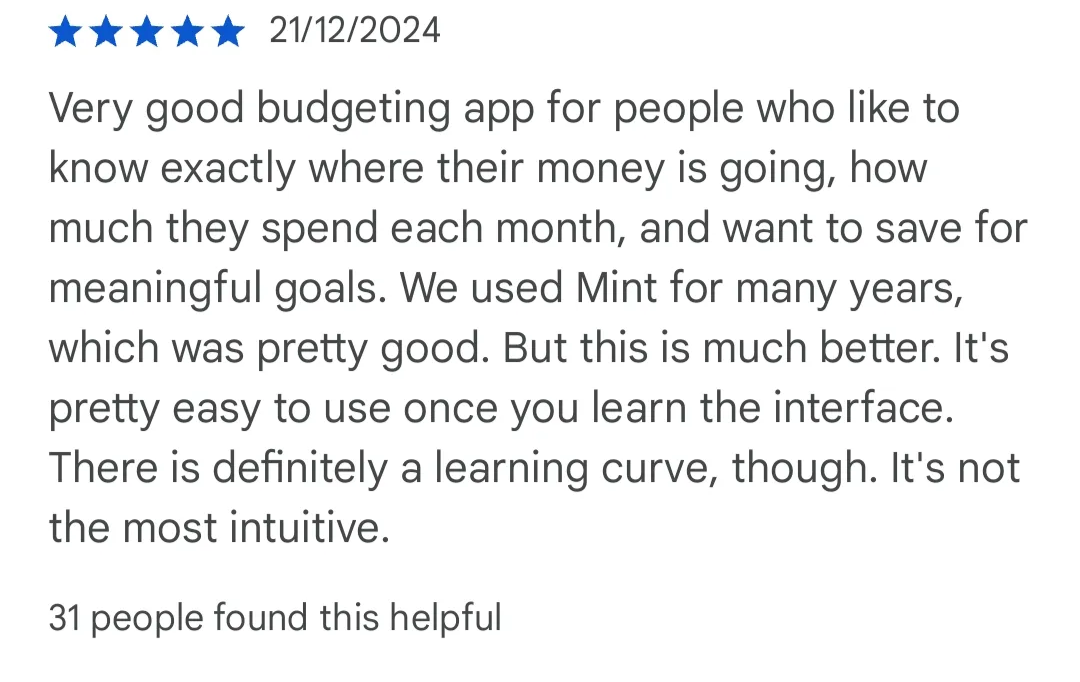
\includegraphics[width=0.5\linewidth]{images/App-Comparison/ynab-review-2.png}
    \caption{Review noting that the app has a rather steep learning curve.}
    \label{fig:enter-label}
\end{figure}
\begin{figure}[H]
    \centering
    \includegraphics[width=0.5\linewidth]{images/App-Comparison/ynab-review-3.png}
    \caption{Review complaining that the app is too expensive and that the zero-budgeting approach was frustrating for this user.}
    \label{fig:enter-label}
\end{figure}

\chapter{User Research Questionnaire \& Ethics Scripts}
\label{app:user-survey}
\includepdf[pages=-]{Data/Budgeting with Technology User Survey.pdf}

\chapter{User Research Questionnaire Results}
\label{app:user-survey-results}
\section{Link To Microsoft Form Results}
Microsoft Form summary results can be found \href{https://forms.office.com/Pages/AnalysisPage.aspx?AnalyzerToken=KkePlypYV4CgKDFyU41zF1OEeqhQEk9q&id=KVxybjp2UE-B8i4lTwEzyLzaCqY070xHgthppmcrVEpUMzZLU0NSUDlKTkpITFA4NUVLWFc5Q000RC4u}{here}. 

\section{Detailed Results Summary}
The survey received a total of 51 responses. The results showed that 88\% of respondents were aged between 18 and 25, and only 6 respondents were over the age of 36 (see Figure \ref{fig:age-ranges}). Confidence with technology was very high as can be seen in Figure \ref{fig:comfort-tech}. Interestingly, there was a strong correlation between comfort with technology and the use of budgeting apps. Any respondents who currently use a budgeting app stated that they were very comfortable using technology and the only participants to say that were completely unwilling to even try using a budgeting app were over 36 years old.

\begin{figure}
    \centering
    \includegraphics[width=0.5\linewidth]{images/User-Survey/user-survey-charts-age-range.png}
    \caption{Chart showing the distribution of ages of respondents.}
    \label{fig:age-ranges}
\end{figure}

The majority of respondents use their mobile phone to manage their finances, as can be seen in Figure \ref{fig:devices}, with the next most common device used being a laptop. These findings highlight the importance of designing a budgeting app that is mobile-friendly.

\begin{figure}[htb] 
    \centering
    \begin{subfigure}[b]{0.47\textwidth}
        \centering
        \includegraphics[width=\linewidth]{images/User-Survey/user-survey-charts-comfort-tech.png}
        \caption{How comfortable respondents reported feeling with using technology.}
        \label{fig:comfort-tech}
    \end{subfigure}
    \begin{subfigure}[b]{0.45\textwidth}
        \centering
        \includegraphics[width=\linewidth]{images/User-Survey/user-survey-charts-devices.png}
        \caption{The types of devices respondents use to manage their finances.}
        \label{fig:devices}
    \end{subfigure}
    \caption{Column charts illustrating respondents comfort with technology and the devices they use to manage their finances.}
    \label{fig:comf-devices-charts}
\end{figure}

A slight majority of 55\% of the respondents budget in some form, with 45\% stating that they carry out no budgeting of any kind. Among those who do budget, most review their finances either monthly (43\%) or weekly (36\%), as seen in Figure \ref{fig:budgeting-periods}. This shows that it is important that the budgeting app allows for these reporting periods.

The most common tools used to budget were reported to be spreadsheets (32\%) and pen and paper (29\%), as can be seen in Figure \ref{fig:methods}. Other less frequent methods included banking apps, budgeting apps, notes apps, and mental calculations.

\begin{figure}
    \centering
    \includegraphics[width=0.5\linewidth]{images/User-Survey/user-survey-charts-methods.png}
    \caption{Chart showing the different tools and methods respondents use to budget.}
    \label{fig:methods}
\end{figure}

\begin{figure}[htb] 
    \centering
    \begin{subfigure}[b]{0.45\textwidth}
        \centering
        \includegraphics[width=\linewidth]{images/User-Survey/user-survey-charts-budgeting-periods.png}
        \caption{How frequently respondents who budget review their finances.}
        \label{fig:budgeting-periods}
    \end{subfigure}
    \begin{subfigure}[b]{0.45\textwidth}
        \centering
        \includegraphics[width=\linewidth]{images/User-Survey/user-survey-charts-sats-tools.png}
        \caption{Respondents’ satisfaction with their current budgeting methods.}
        \label{fig:sats-tools}
    \end{subfigure}
    \caption{Column charts illustrating how often respondents review their finances and how satisfied they are with their current budgeting methods.}
    \label{fig:comf-devices-charts}
\end{figure}

Respondents satisfaction with their budgeting methods can be seen in Figure \ref{fig:sats-tools}. The majority reported that they were at least somewhat satisfied with their current methods, but a notable 25\% were unsatisfied, presenting a clear opportunity to design a tool that addresses common shortcomings and improves user experience.

Respondents who budget indicated a number of motivations, with the most common being:
\begin{itemize}
    \item Tracking spending/visualising where money goes (56\%)
    \item Saving, either long-term or for specific goals (52\%)
    \item Ensuring bills are paid (29.6\%)
\end{itemize}

Other goals included reducing unnecessary purchases, building an emergency fund, and having enough disposable income for hobbies/treat items.

Despite the prevalence of budgeting habits, only 11\% of those who budget currently use a budgeting app. The most common reasons given for not using one were:
\begin{itemize}
    \item Lack of awareness or felt there was no need for one (43.5\%)
    \item Preference for existing methods such as spreadsheets or banking apps (35\%)
    \item The complexity or stress associated with budgeting apps (17.4\%)
    \item Privacy concerns and lack of personalisation were also mentioned by some participants.
\end{itemize}

A large portion of respondents indicated openness to trying a budgeting app in the future: 40\% said they would, and 52\% said they might. Only 8\% firmly rejected the idea.

Among those who do not currently budget, the most common barriers stated were:
\begin{itemize}
    \item There is too much effort involved in using a budgeting app (35\%)
    \item A lack of necessity based on personal financial circumstances (26\%)
    \item Feeling overwhelmed by the process (22\%)
\end{itemize}

In terms of motivators, the majority of non-budgeters indicated they would consider budgeting if:
\begin{itemize}
    \item They had access to a helpful tool (45\%)
    \item Their financial situation changed (36\%)
    \item They gained more knowledge or confidence in budgeting (14\%)
\end{itemize}

Participants provided detailed feedback on the features they would find most valuable in a budgeting application. These included:
\begin{itemize}
    \item Linked banking integration (15\%)
    \item Categorising expenses into different money pots (12\%)
    \item Reports and charts on spending (12\%), including predictive models showing how finances may evolve based on decisions
    \item Notifications and alerts, such as:
    \begin{itemize}
        \item When limits are reached
        \item Reminders about upcoming bills or payments
        \item Weekly spending summaries and progress updates
    \end{itemize}
    \item Budgeting tips and educational features, including personalised insights and advice on how to save more effectively.
\end{itemize}

Participants also expressed a strong preference for simplicity, clarity, and for the app to be free to use.

When asked to rank a number of features by what the respondents felt was most important to them in a budgeting app, the average ranking was:
\begin{enumerate}
    \item Reports and charts on spending and income
    \item Savings goal setting
    \item Envelope budgeting (i.e., assigning spending limits by category)
    \item Tracking multiple bank accounts
\end{enumerate}

Additional suggestions included:
\begin{itemize}
    \item Ability to visualise income vs. expenses dynamically throughout the month
    \item Exportable data and reports
    \item Insights into where money is spent (e.g., by shop or category)
    \item Educational resources or budgeting advice embedded within the app
\end{itemize}

\chapter{Architecture Diagrams}
\label{app:architecture}
\begin{figure}[htb] 
    \centering
    \begin{subfigure}[b]{0.75\textwidth}
        \includegraphics[width=\textwidth]{images/Architecture-Diagrams/Architecture_Diagram.jpeg}
        \label{fig:syn1}
    \end{subfigure}   
    \caption{Initial architecture design using a React front-end.}\label{fig:synthetic}
\end{figure}
\begin{figure}[htb] 
    \centering
    \begin{subfigure}[b]{0.75\textwidth}
        \includegraphics[width=\textwidth]{images/Architecture-Diagrams/Architecture_Diagram_PWA.png}
        \label{fig:syn1}
    \end{subfigure}   
    \caption{Final architecture design using an Angular front-end with the PWA labelled. \\ \\
    \textbf{Service Worker} - manages offline access, push notifications and caching of the PWA. \\
    \textbf{Manifest} - enables installable app on mobile and desktop.}
    \label{fig:synthetic}
\end{figure}

\chapter{Wireframes}
\label{app:wireframes}
\section{Login Page}
\begin{figure}[htb]
    \centering
    \includegraphics[width=0.75\linewidth]{images/Wireframes/wireframe-login-desktop.png}
    \caption{Desktop wireframe for the login page.}
    \label{fig:enter-label}
\end{figure}

\begin{figure}[htb]
    \centering
    \includegraphics[width=0.35\linewidth]{images/Wireframes/wireframe-login-phone.png}
    \caption{Phone wireframe for the login page.}
    \label{fig:enter-label}
\end{figure}
\newpage

\section{Home Page}
\begin{figure}[htb]
    \centering
    \includegraphics[width=0.75\linewidth]{images/Wireframes/wireframe-home-desktop.png}
    \caption{Desktop wireframe for the home page.}
    \label{fig:enter-label}
\end{figure}

\begin{figure}[htb]
    \centering
    \includegraphics[width=0.35\linewidth]{images/Wireframes/wireframe-home-phone.png}
    \caption{Phone wireframe for the home page.}
    \label{fig:enter-label}
\end{figure}
\newpage

\section{Income Page}
\begin{figure}[htb]
    \centering
    \includegraphics[width=0.75\linewidth]{images/Wireframes/wireframe-income-desktop.png}
    \caption{Desktop wireframe for the income page.}
    \label{fig:enter-label}
\end{figure}

\begin{figure}[htb]
    \centering
    \includegraphics[width=0.3\linewidth]{images/Wireframes/wireframe-income-phone.png}
    \caption{Phone wireframe for the income page.}
    \label{fig:enter-label}
\end{figure}
\vspace{0.5em}
\textbf{Note:} The UIs for the expenses and savings pages are very similar.

\newpage

\section{Log a Transaction Page}
\begin{figure}[htb]
    \centering
    \includegraphics[width=0.75\linewidth]{images/Wireframes/wireframe-trans-desktop.png}
    \caption{Desktop wireframe for the log a transaction page.}
    \label{fig:enter-label}
\end{figure}

\begin{figure}[htb]
    \centering
    \includegraphics[width=0.3\linewidth]{images/Wireframes/wireframe-trans-phone.png}
    \caption{Phone wireframe for the log a transaction page.}
    \label{fig:enter-label}
\end{figure}
\newpage

\section{Budget Page}
\begin{figure}[htb]
    \centering
    \includegraphics[width=0.75\linewidth]{images/Wireframes/wireframe-budget-desktop.png}
    \caption{Desktop wireframe for the budget page.}
    \label{fig:enter-label}
\end{figure}

\begin{figure}[htb]
    \centering
    \includegraphics[width=0.3\linewidth]{images/Wireframes/wireframe-budget-phone.png}
    \caption{Phone wireframe for the budget page.}
    \label{fig:enter-label}
\end{figure}
\newpage


\section{Reports Page}
\begin{figure}[htb]
    \centering
    \includegraphics[width=0.75\linewidth]{images/Wireframes/wireframe-reports-desktop.png}
    \caption{Desktop wireframe for the reports page.}
    \label{fig:enter-label}
\end{figure}

\begin{figure}[htb]
    \centering
    \includegraphics[width=0.3\linewidth]{images/Wireframes/wireframe-reports-phone.png}
    \caption{Phone wireframe for the reports page.}
    \label{fig:enter-label}
\end{figure}
\newpage

\section{Redesigned Nav Bar}
\label{app:wireframes-nav-bar}
\begin{figure}[htb] 
    \centering
    \begin{subfigure}[b]{0.8\textwidth}
        \includegraphics[width=\textwidth]{images/Wireframes/wireframe-nav-desktop.png}
    \end{subfigure}   
    \caption{Updated Nav Bar Wireframe.}\label{fig:nav-bar}
\end{figure}

\chapter{Logo Inspiration}
\label{app:logo-inspiration}
\textbf{Disclaimer:} The following images were sourced via Google and are used here for illustrative purposes only. I do not claim ownership of these images.

\begin{figure}[H]
    \centering
    \includegraphics[width=0.3\linewidth]{images/Logo/inspo-1.png}
    \caption{Image found on \href{https://www.dreamstime.com/evergreen-pine-tree-logo-design-inspiration-evergreen-pine-tree-logo-design-inspiration-vector-image134609964}{Dreamstime}.}
    \label{fig:enter-label}
\end{figure}
\begin{figure}[H]
    \centering
    \includegraphics[width=0.3\linewidth]{images/Logo/inspo-2.png}
    \caption{An \href{https://stock.adobe.com/uk/search?k=evergreen+tree+logo}{Adobe Stock} image.}
    \label{fig:enter-label}
\end{figure}
\begin{figure}[H]
    \centering
    \includegraphics[width=0.2\linewidth]{images/Logo/inspo-3.png}
    \caption{Logo of \href{https://www.ynab.com/}{YNAB}.}
    \label{fig:enter-label}
\end{figure}
\begin{figure}[H]
    \centering
    \includegraphics[width=0.3\linewidth]{images/Logo/inspo-4.png}
    \caption{Logo of \href{https://www.ebcmaine.com/about}{Evergreen Building Co.}}
    \label{fig:enter-label}
\end{figure}

\chapter{Software Engineering Processes}
\section{Issues}
\label{app:issues}
\begin{figure}[h]
    \centering
    \includegraphics[width=0.75\linewidth]{images/GitHub-Screenshots/issue-commit-messages.png}
    \caption{An issue showing the description, milestone, priority tag, time estimation tag and the history of commits related to the issue.}
    \label{fig:issue}
\end{figure}

\begin{figure}[h]
    \centering
    \includegraphics[width=0.9\linewidth]{images/GitHub-Screenshots/issue-closing-comment.png}
    \caption{Issue showing a non-code task being closed with a comment that explains the actions taken.}
    \label{fig:enter-label}
\end{figure}

\begin{figure}[h]
    \centering
    \includegraphics[width=0.9\linewidth]{images/GitHub-Screenshots/issue-amending-work.png}
    \caption{Issue illustrating documentation through commits.}
    \label{fig:enter-label}
\end{figure}

\chapter{UI Screenshots}
\label{app:ui-screenshots}
\section{Login \& Registration Pages}
\begin{figure}[htb]
    \centering
    \includegraphics[width=0.35\linewidth]{images/UI-Screenshots/registration-page.png}
    \caption{The implemented registration page. Note the default currency field.}
    \label{fig:registration-page}
\end{figure}

\begin{figure}[htb]
    \centering
    \includegraphics[width=0.75\linewidth]{images/UI-Screenshots/login-page.png}
    \caption{The implemented login page. Note that the nav bar matches the redesign.}
    \label{fig:login-page}
\end{figure}

\section{Home Page}
\begin{figure}[H]
    \centering
    \includegraphics[width=\linewidth]{images/UI-Screenshots/home-page.png}
    \caption{The implemented home page. Each main page of the app has a small overview on the home page. There is also a table in the top-right that gives an overview of the users income and outgoings for the month. Note the new nav bar design.}
    \label{fig:reports-page}
\end{figure}

\section{Expenses/Income Page}
\begin{figure}[H]
    \centering
    \includegraphics[width=\linewidth]{images/UI-Screenshots/expenses-page.png}
    \caption{The implemented expenses page.}
    \label{fig:reports-page}
\end{figure}

\begin{figure}[H]
    \centering
    \includegraphics[width=\linewidth]{images/UI-Screenshots/income-page.png}
    \caption{The implemented income page.}
    \label{fig:reports-page}
\end{figure}

\begin{figure}[htb]
    \centering
    \includegraphics[width=0.5\linewidth]{images/UI-Screenshots/delete-transaction.png}
    \caption{The popup that confirms the deletion of a transaction. For repeated transactions, the user is given the options as seen in the checkbox list.}
    \label{fig:transaction-delete}
\end{figure}

\section{Savings Page}
\begin{figure}[H]
    \centering
    \includegraphics[width=\linewidth]{images/UI-Screenshots/savings-page.png}
    \caption{The implemented savings page. Note the savings goal area at the bottom of the screen.}
    \label{fig:reports-page}
\end{figure}

\begin{figure}[htb]
    \centering
    \includegraphics[width=0.5\linewidth]{images/UI-Screenshots/savings-goals-home.png}
    \caption{The savings section on the home page. The progress bar indicates how close the user is to meeting their aggregated savings goal.}
    \label{fig:savings-goals-home}
\end{figure}

\section{Budget Page}
\begin{figure}[H]
    \centering
    \includegraphics[width=\linewidth]{images/UI-Screenshots/budget-page-fullscreen.png}
    \caption{The implemented budget page with watering cans representing spending in each budget category.}
    \label{fig:reports-page}
\end{figure}

\section{Reports Page}
\begin{figure}[H]
    \centering
    \includegraphics[width=\linewidth]{images/UI-Screenshots/reports-page-fullscreen.png}
    \caption{The implemented reports page.}
    \label{fig:reports-page}
\end{figure}

\section{Mobile-App \& Issues}
\begin{figure}[htb] 
    \centering
    \begin{subfigure}[b]{0.3\textwidth}
        \fbox{\includegraphics[width=\textwidth]{images/UI-Screenshots/phone-disjointed.png}}
        \caption{Illustrates the disjointed alignment of components.}
        \label{fig:mobile-disjointed}
    \end{subfigure}
    \hspace{1em}
    \begin{subfigure}[b]{0.3\textwidth}
        \fbox{\includegraphics[width=\textwidth]{images/UI-Screenshots/nav-bar-phone.png}}
        \caption{Shows the navigation bar on smaller screens.}
        \label{fig:nav-bar-phone}
    \end{subfigure}   
    \caption{\subref{fig:mobile-disjointed} This misalignment is due to the sizing of the AG Grid tables, see the "Upcoming Savings" table, and the drag-and-drop areas, which are not visible as these are lower down the web page. \subref{fig:nav-bar-phone} shows the nav bar for smaller screens, note that only the logo and hamburger menu are displayed.
    }\label{fig:screenshots}
\end{figure}
\clearpage
\section{Authentication Middleware Code Listing}
\label{app:auth-middleware}
\begin{lstlisting}[language=Java, float, caption={The code in the authentication middleware which is used in the router.post calls as seen in Listing \ref{lst:authenticate-route}. If a token is provided, this code verifies it matches the token generated at login. If it does not, it throws an error.}, label=lst:authenticate-middleware]
    const authenticateToken = (req, res, next) => {

        const authHeader = req.headers['authorization'];
        const token = authHeader && authHeader.split(' ')[1];
        if (!token) return res.status(401).json({ error: 'Access token required'});
        
        jwt.verify(token, secretKey, (err, user) => {
            if (err) return res.status(403).json({ error: 'Invalid token' });
            req.user = user;
            next();
        });
    };
\end{lstlisting}

\chapter{Testing Code Coverage}

\section{Frontend Metrics}
\label{app:code-coverage-frontend}
\begin{figure}[H]
    \centering
    \includegraphics[width=\linewidth]{images/Code-Coverage/coverage-frontend.png}
    \caption{Coverage metrics for unit tests of Angular components.}
    \label{fig:reports-page}
\end{figure}

\begin{figure}[H]
    \centering
    \includegraphics[width=\linewidth]{images/Code-Coverage/coverage-frontend-services.png}
    \caption{Coverage metrics for the frontend Angular services.}
    \label{fig:reports-page}
\end{figure}

\section{Server Metrics}
\label{app:code-coverage-server}
\begin{figure}[H]
    \centering
    \includegraphics[width=\linewidth]{images/Code-Coverage/coverage-server.png}
    \caption{The overview of coverage metrics for the backend server.}
    \label{fig:reports-page}
\end{figure}

\begin{figure}[H]
    \centering
    \includegraphics[width=\linewidth]{images/Code-Coverage/coverage-server-api.png}
    \caption{Coverage metrics for the API server files.}
    \label{fig:reports-page}
\end{figure}

\begin{figure}[H]
    \centering
    \includegraphics[width=\linewidth]{images/Code-Coverage/coverage-server-queries.png}
    \caption{Coverage metrics for the server query files.}
    \label{fig:reports-page}
\end{figure}

\chapter{Evaluation Ethics Checklist}
\label{app:ethics-checklist}
\includepdf[pages=-]{Data/ethics-checklist-signed.pdf}

\chapter{Evaluation Questionnaires \& Results}
\label{app:ethics-questionnaires}
\section{In-Person Evaluation}
\includepdf[pages=-]{Data/Evaluation - In-Person.pdf}

\section{Remote Evaluation}
\includepdf[pages=-]{Data/Evaluation - Remote.pdf}

\section{Links to Results}
\label{app:result-links}

\subsection{Supervised Evaluation Microsoft Form Results}
\url{https://forms.office.com/Pages/AnalysisPage.aspx?AnalyzerToken=1GuUBmawOfbSi2YK6Qt061tDcgVVl1q4&id=KVxybjp2UE-B8i4lTwEzyLzaCqY070xHgthppmcrVEpUOVpYNElCVUZXQ0JQRkI5T1A1MjNaREcyVy4u}

\subsection{Unsupervised Evaluation Microsoft Form Results}
\url{https://forms.office.com/Pages/AnalysisPage.aspx?AnalyzerToken=wz7TPfdjadrJxikAVfc1UFHjoNqL9jlh&id=KVxybjp2UE-B8i4lTwEzyLzaCqY070xHgthppmcrVEpUMjhPUjBYMEs3MVQ3RFNNRVFRWUgzTDAwUi4u}

\subsection{Combined \& Summarised Results}
Hosted with Notion: \url{https://dolomite-account-777.notion.site/Evaluation-Discussion-1c11f372b4378030b435e0c72b0c915a?pvs=4}

\chapter{Evaluation Charts}
\label{app:evaluation-charts}
\begin{figure}[H]
    \centering
    \includegraphics[width=0.75\linewidth]{images/Evaluation-Charts/age-ranges.png}
    \caption{Chart showing the distribution of participants' ages.}
    \label{fig:enter-label}
\end{figure}

\begin{figure}[H]
    \centering
    \includegraphics[width=0.75\linewidth]{images/Evaluation-Charts/budget-methods.png}
    \caption{Chart showing the most common budgeting methods amongst the participants}
    \label{fig:enter-label}
\end{figure}

\begin{figure}[H]
    \centering
    \includegraphics[width=0.75\linewidth]{images/Evaluation-Charts/budget-time-periods.png}
    \caption{Chart showing how often the participants review their budgets.}
    \label{fig:enter-label}
\end{figure}

\begin{figure}[H]
    \centering
    \includegraphics[width=0.75\linewidth]{images/Evaluation-Charts/remote-devices.png}
    \caption{Chart showing the devices used to conduct the evaluation by unsupervised participants.}
    \label{fig:enter-label}
\end{figure}

\begin{figure}[H]
    \centering
    \includegraphics[width=0.75\linewidth]{images/Evaluation-Charts/ease-repeated-trans.png}
    \caption{Chart depicting how easy participants found adding repeat transactions.}
    \label{fig:enter-label}
\end{figure}

\begin{figure}[H]
    \centering
    \includegraphics[width=0.75\linewidth]{images/Evaluation-Charts/clear-budget.png}
    \caption{Chart showing the preferred page to view budget information.}
    \label{fig:enter-label}
\end{figure}

\begin{figure}[H]
    \centering
    \includegraphics[width=0.75\linewidth]{images/Evaluation-Charts/ease-navigation.png}
    \caption{Chart illustrating ease of navigation across the site.}
    \label{fig:enter-label}
\end{figure}

\begin{figure}[H]
    \centering
    \includegraphics[width=0.75\linewidth]{images/Evaluation-Charts/preferred-version.png}
    \caption{Participants' preferences for the computer or phone version of the application.}
    \label{fig:enter-label}
\end{figure}

\begin{figure}[H]
    \centering
    \includegraphics[width=0.75\linewidth]{images/Evaluation-Charts/replace-method.png}
    \caption{Chart showing the proportion of participants who would use the app to manage their finances.}
    \label{fig:enter-label}
\end{figure}

\begin{figure}[H]
    \centering
    \includegraphics[width=0.75\linewidth]{images/Evaluation-Charts/phone-convenience.png}
    \caption{Chart showing if participants found using the mobile version of the app convenient.}
    \label{fig:enter-label}
\end{figure}

\chapter{Guides}
\section{Manual}
\includepdf[pages=-]{Data/manual.pdf}

\end{appendices}

%==================================================================================================================================
%   BIBLIOGRAPHY   

% The bibliography style is agsm (Harvard)
% The bibliography always appears last, after the appendices.

\bibliographystyle{agsm}

% Force the bibliography not to be numbered
\renewcommand{\thechapter}{0}
\bibliography{l4proj}

\end{document}
